\documentclass[12pt,fleqn,a4paper,twoside]{mybook} %Final!!!

%\usepackage{microtype}
%\usepackage{lmodern}
\usepackage[slovak]{babel}
\usepackage[utf8]{inputenc}
\usepackage[T1]{fontenc}
\usepackage{lmodern}
\pdfgentounicode=1
%\usepackage[normalem]{ulem}
\usepackage{mathtools}  					
\usepackage{graphicx}
%\usepackage{subfig}
\usepackage{subfigure}
\usepackage{pdfpages}
\usepackage{enumerate}
\usepackage{etoolbox}                       %Problematic URL in reference
\apptocmd{\sloppy}{\hbadness 10000\relax}{}{}%Removes badness warnings
%This is to remove warnings resulting by otherwise OK URL's
\usepackage[hyphens]{url}
\usepackage{notes}
\usepackage{indentfirst}
\usepackage{makecell}
\renewcommand\theadfont{\bfseries\sffamily}
%\usepackage[demo]{graphicx}
\usepackage{upgreek}
\usepackage{multicol}
\usepackage{eurosym}
%This custom command defines how the literal menus look like.
\newcommand{\gui}[1]{{\emph{#1}}} %Gui commands, icon names, buttons
 % All code, functions, variables are typed like this
\newcommand{\code}[1]{{\lstinline[columns=fixed]{#1}}}

\newcommand{\angl}[1]{{\footnote{\emph{angl.}\ {#1}}}} %Shorthand english equivalent


\usepackage[inner=3.5cm,outer=2cm,top=25mm,bottom=25mm,paperwidth=210mm,paperheight=297mm,includehead]{geometry}

\usepackage{titlesec}
\titleformat{\chapter}[hang]{\normalfont\huge\bfseries}{\thechapter}{1em}{}


\DeclarePairedDelimiter{\diagpars}{(}{)}
\newcommand{\diag}{\operatorname{diag}\diagpars}

\let\oldhat\hat
\renewcommand{\vec}[1]{\boldsymbol{\mathbf{#1}}}
%\renewcommand{\hat}[1]{\oldhat{\boldsymbol{\mathbf{#1}}}}


\usepackage{amsthm}
\usepackage{etoolbox}% http://ctan.org/pkg/etoolbo
\theoremstyle{definition}
\newtheorem{exmp}{Pr\'{i}klad}[chapter]
\AtEndEnvironment{exmp}{\null\hfill\qedsymbol}

\usepackage{listings,color} 			    %To list Matlab code


\usepackage{xcolor}

\definecolor{Myblack}{RGB}{48, 55, 54}
\definecolor{Mybrown}{RGB}{15, 153, 117}
\definecolor{Mygreen}{RGB}{160, 82, 131}
\definecolor{Myyellow}{RGB}{208, 170, 91}
\definecolor{Myblue}{RGB}{4, 118, 249}

\lstset{language=C++,
	basicstyle=\ttfamily,
	keywordstyle=\color{Myblue}\ttfamily,
	stringstyle=\color{Myyellow}\ttfamily,
	commentstyle=\color{Mygreen}\ttfamily,
	numbers=none,
	breaklines=true,
	showspaces=false,
	showstringspaces=false
	backgroundcolor=\color{white}, % set backgroundcolor
	basicstyle=\footnotesize,% basic font setting
	morecomment=[l][\color{Mybrown}]{\#}
}

\renewcommand\lstlistingname{Zdrojový kód}
\renewcommand\lstlistlistingname{Zoznam zdrojového kódu}

\pagestyle{empty}

\begin{document}
%%%%%%% Zaciaatok %%%%%%%%
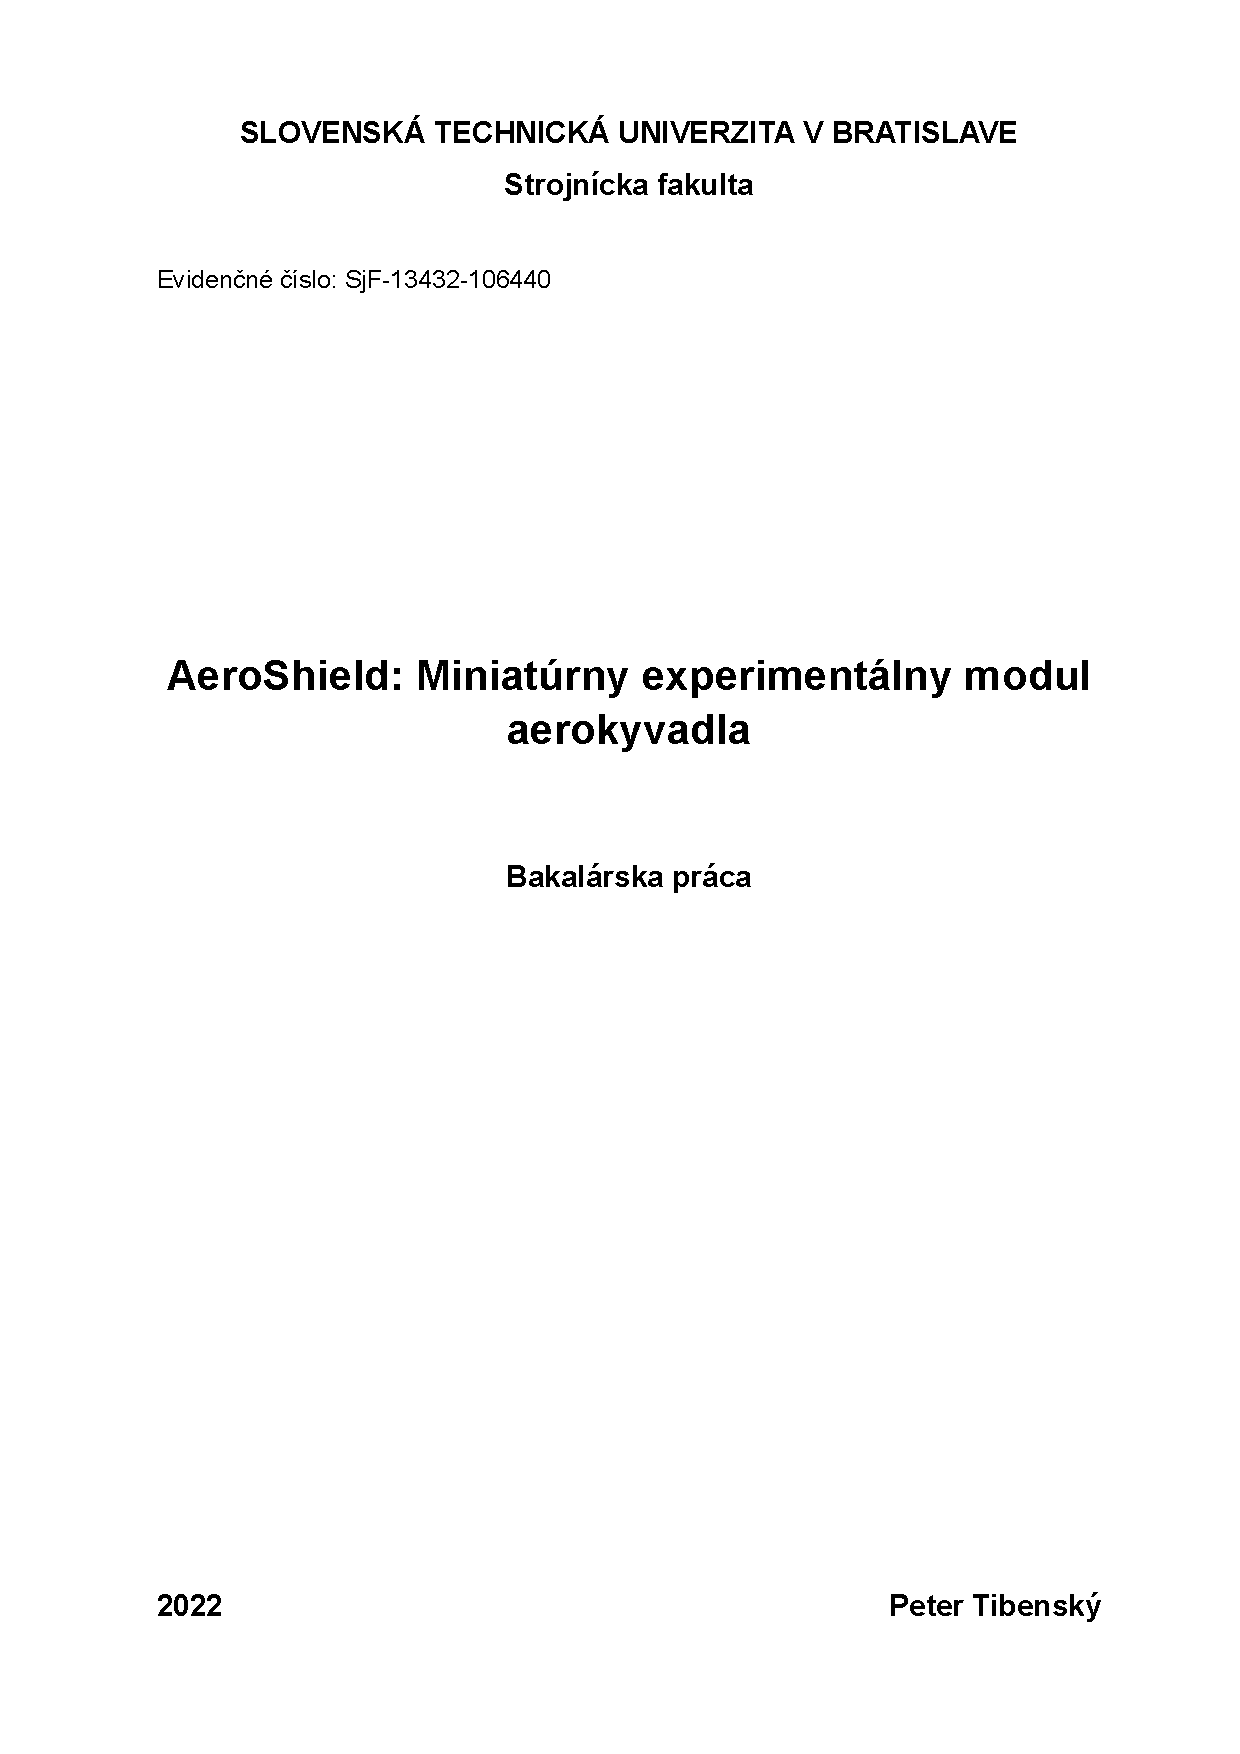
\includepdf[pages=-]{Titulka.pdf}

\includepdf[pages=-]{Blank.pdf}
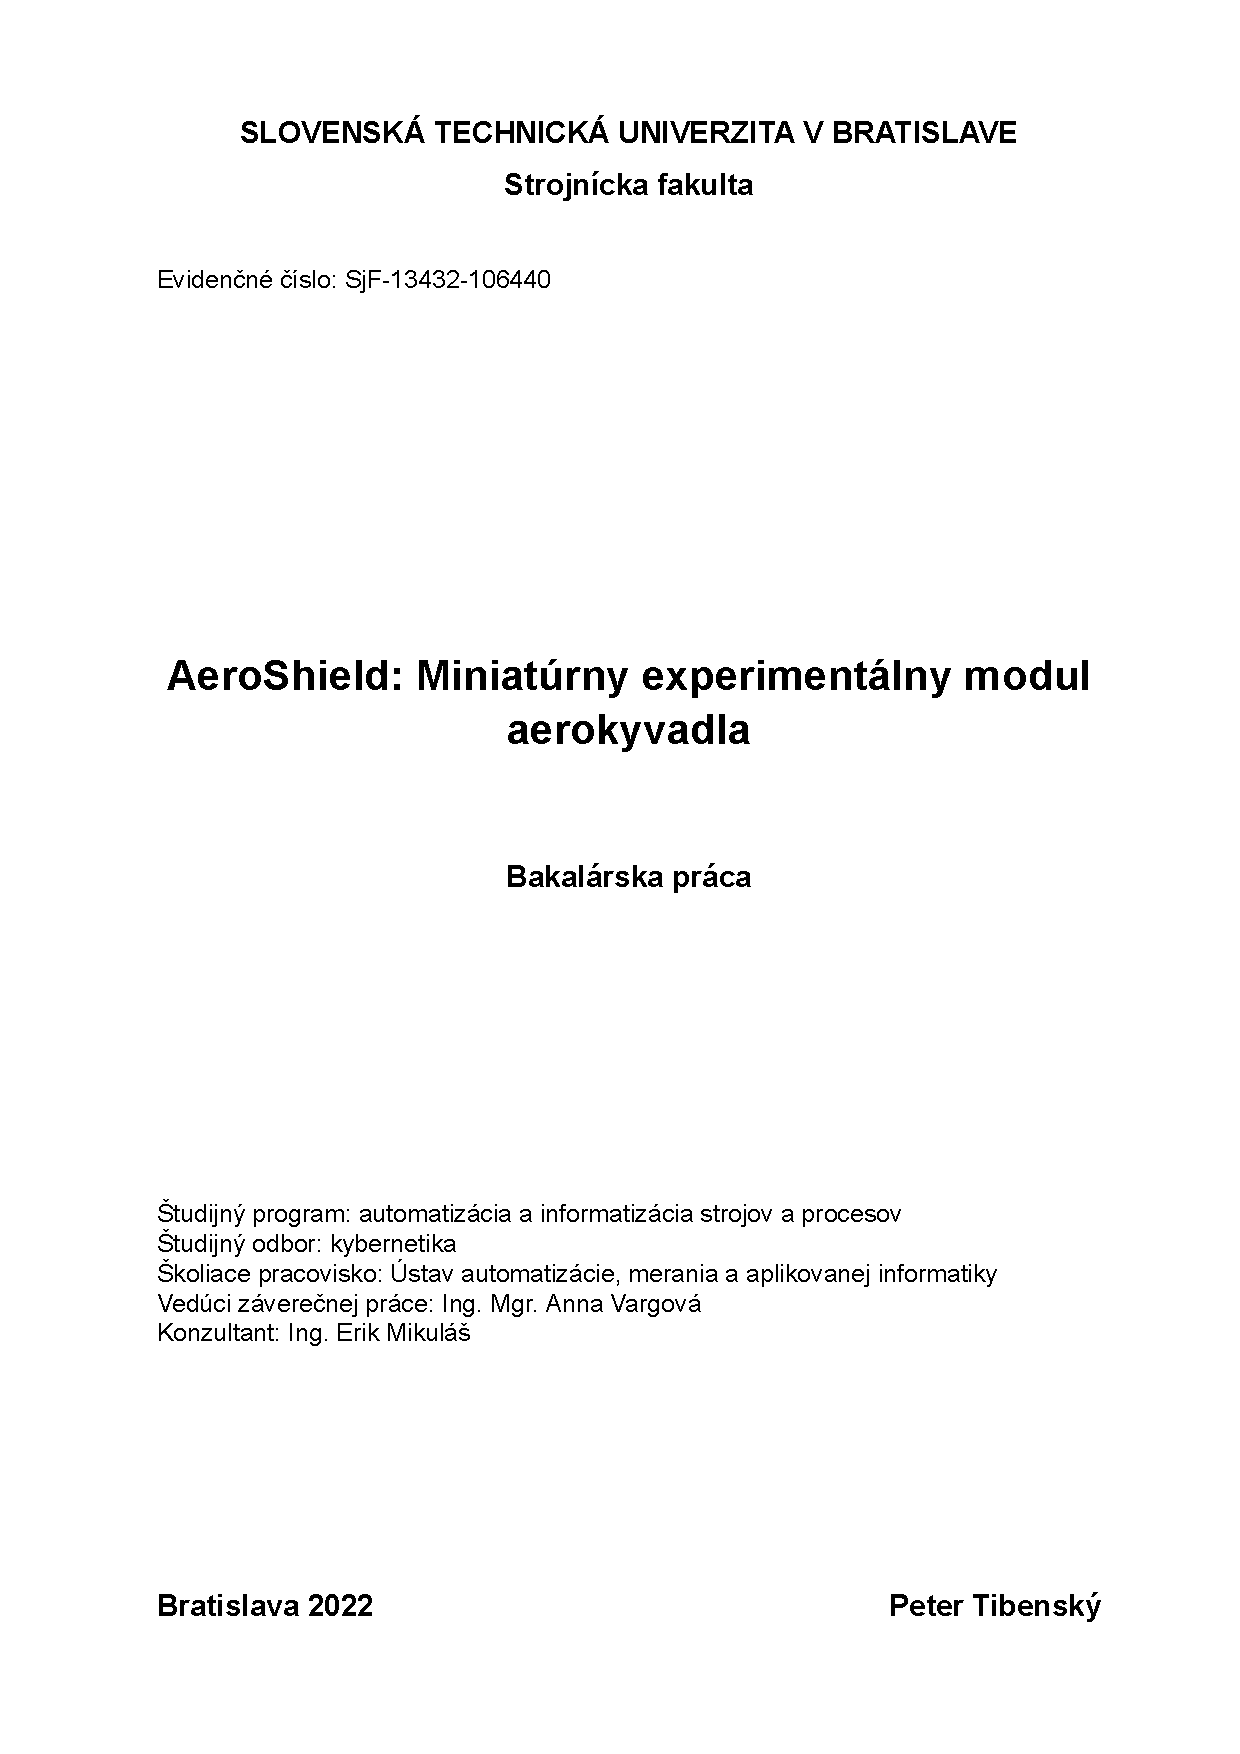
\includepdf[pages=-]{druhaTitulka.pdf}

\includepdf[pages=-]{Blank.pdf}
\frontmatter
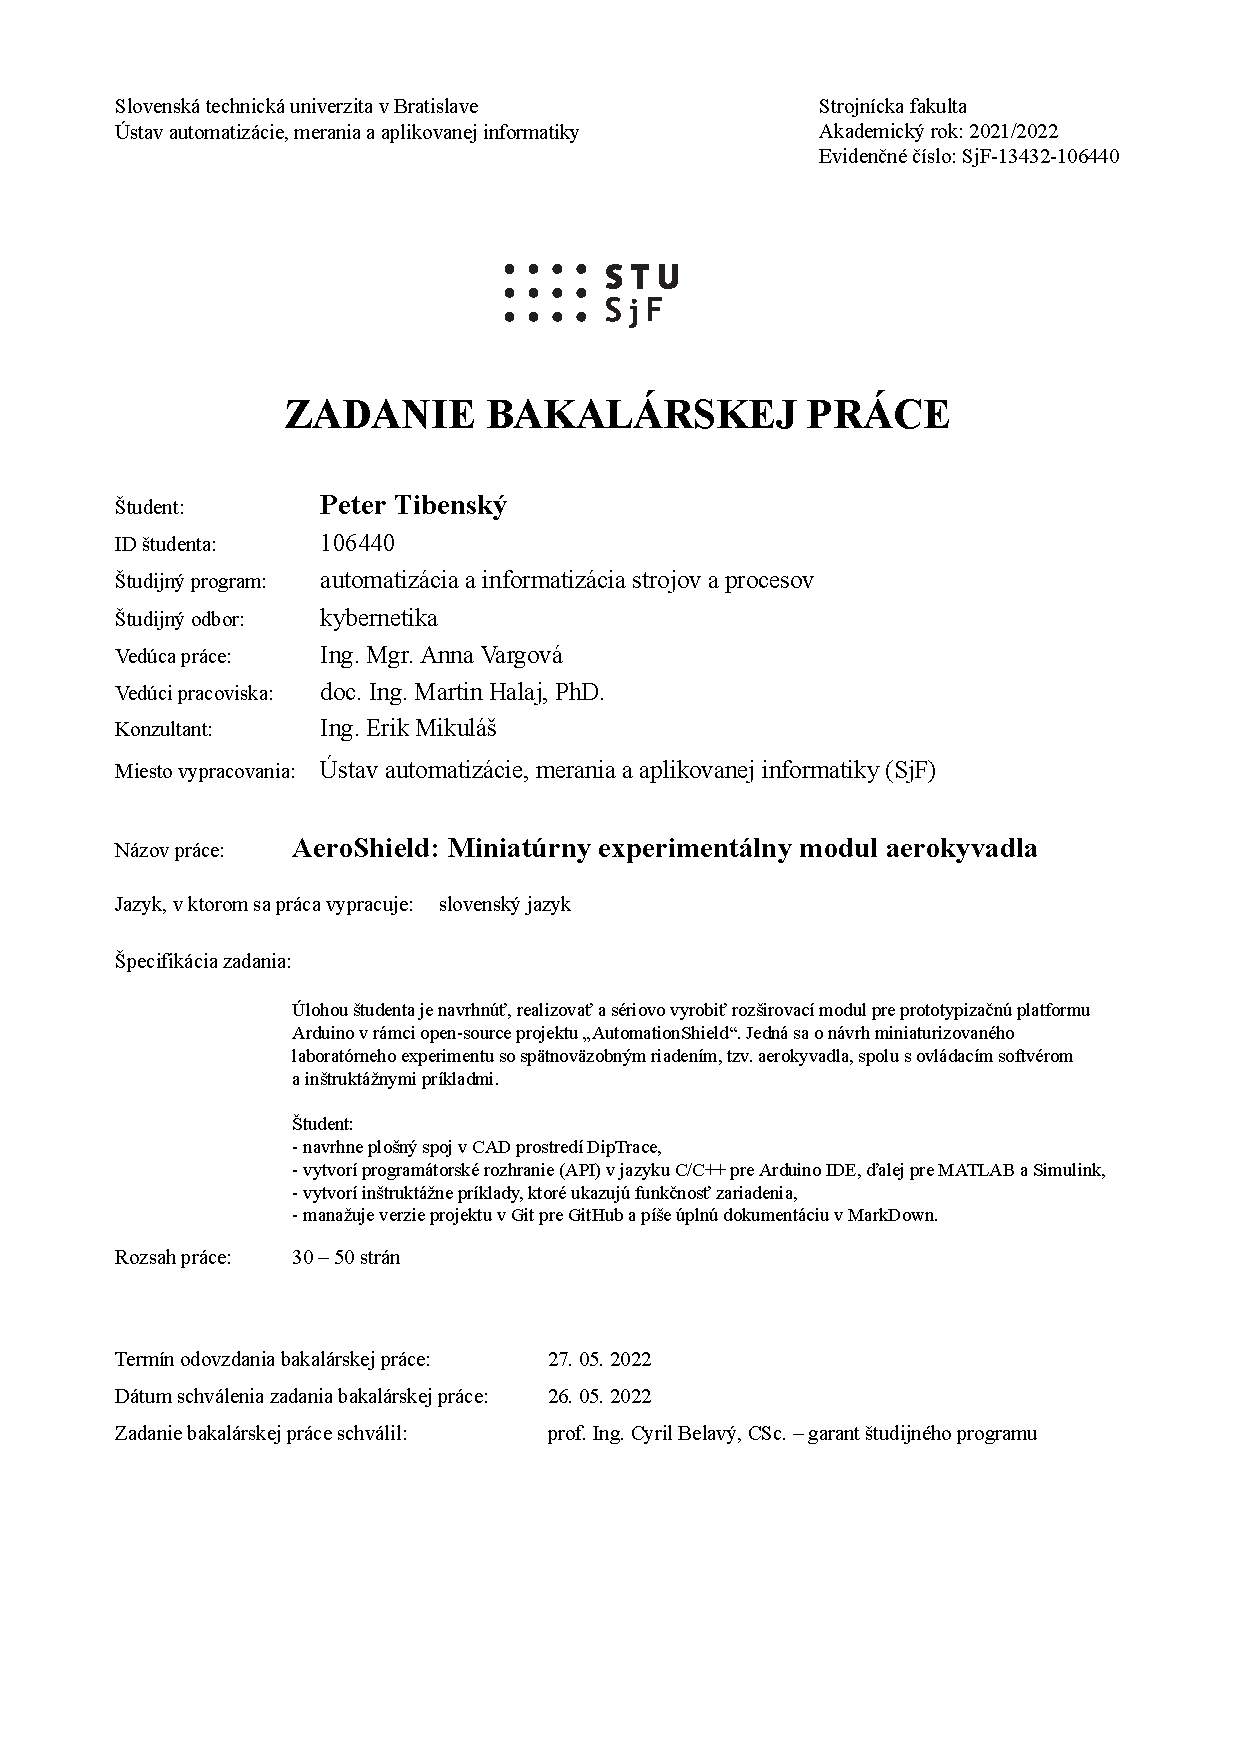
\includepdf[pages=-]{ZadanieOmg.pdf}

\includepdf[pages=-]{Blank.pdf}
 \null
\vfill
\noindent
\section*{Čestné prehlásenie}

Vyhlasujem, že predloženú záverečnú prácu som vypracoval samostatne pod vedením vedúceho záverečnej práce, s použitím odbornej literatúry a ďalších informačných zdrojov, ktoré sú citované v práci a uvedené v zozname použitej literatúry. Ako autor záverečnej práce ďalej prehlasujem, že som v súvislosti s jej vytvorením neporušil autorské práva tretích osôb.\\

\noindent Bratislava, 26. máj 2022 \hfill $\begin{array}{rl}
                                          &\text{..................................}\\
                                          &\text{Vlastnoručný podpis}\\
                                           \end{array}$
\cleardoublepage


	

 \null
\vfill
\noindent

V prvom rade by som sa chcel poďakovať vedúcej mojej bakalárskej práce, Ing. Mgr. Anne Vargovej, za výborne kávičky v kabinete, najlepšie meme obrázky v skupine ako aj za cenné rady a nekonečné opravy tejto práce. Ďalej chcem poďakovať aj Ing. Erikovi Mikulášovi, za pomoc pri tvorbe a kontrole (skoro)všetkých elektronických komponentov AeroShieldu, ako aj za pevné ruky pri spájkovaní. Ďakujem aj mojej partnerke Slávke, za to že každý deň trpezlivo počúvala moje nekonečné nadávky, sťažnosti ale aj radosti, pri tvorbe tejto práce. Zároveň sa chcem ospravedlniť spolužiakom, za stres ktorý mali z toho, keď som sa chválil 40. stranou práce, zatiaľ čo podaktorý ešte nepoznali tému ich BP.\\

\noindent Bratislava, 20. mája 2018 \hfill  Peter Tibenský
\cleardoublepage


	


 \noindent
\textbf{Názov práce:} AeroShield: Miniatúrny experimentálny modul aerokyvadla\\
\textbf{Kľúčové slová: } Arduino, AutomationShield, PID, AeroShield, Aero pendulum, softvér, hardvér, Arduino IDE, MATLAB, Simulink \\
\textbf{Abstrakt: } Cieľom bakalárskej práce je návrh experimentálneho modulu pre platformu Arduino. Tento modul má podobu externého shieldu, ktorý sa dá jednoducho pripojiť ku doskám Arduino a slúži na výučbu základov riadenia. Ich súčasťou je hardvérová a softvérová časť. V rámci bakalárskej práce boli navrhnuté dva moduly, AeroShield R2 a R3, ktoré replikujú experiment známy pod názvom aeropendulum. V rámci hardvérovej časti bolo zostavená doska plošných spojov, ako aj celkový model kyvadla. V softvérovej časti boli vytvorené didaktické príklady pre API Arduino IDE ako aj pre MATLAB a Simulink.\\

\noindent
\textbf{Title:}AeroShield: Miniature experimental module of aeropendulum \\
\textbf{Keywords: }  Arduino, AutomationShield, PID, AeroShield, Aero pendulum, software, hardware, Arduino IDE, MATLAB, Simulink\\
\textbf{Abstract: } The aim of this bachelor's thesis is to design an experimental module for the Arduino platform. This module takes the form of an external shield that can be easily connected to Arduino boards and is used to teach the basics of control engineering. Each module consists of hardware and a software part. As a part of this bachelor thesis, two modules were designed, the AeroShield R2 and R3. AeroShield was designed to replicate an experiment known as an aeropendulum. In the hardware part, the printed circuit board (PCB) was designed as well as the overall model of the pendulum. In the software part, didactic examples were created for the API Arduino IDE as well as for MATLAB and Simulink.
\cleardoublepage

%%%%%% \input{Predhovor} %%%%%%
\tableofcontents
\thispagestyle{empty}
\cleardoublepage
\setcounter{page}{1}
% \phantomsection
\addcontentsline{toc}{chapter}{\listfigurename}
\listoffigures
\cleardoublepage
% \phantomsection
\addcontentsline{toc}{chapter}{\lstlistlistingname}
\lstlistoflistings
\newpage
%%%%%% Jednotlive kapitoly %%%%%%%%%
\pagestyle{plain}
\pagenumbering{arabic}
\setcounter{page}{1}

\mainmatter
\chapter*{Úvod}
\label{UVOD}
\addcontentsline{toc}{chapter}{Úvod}

Cieľom tejto práce je návrh, výroba a naprogramovanie modernej učebnej pomôcky AeroShieldu (ďalej len „shield”), ktorá slúži na výučbu základov teórie riadenia a elektrotechniky. Učebné pomôcky sú nevyhnutnou, no často zanedbávanou súčasťou výučby. Študenti si vďaka nim môžu lepšie predstaviť a pochopiť problematiku daného učiva, keďže môžu pracovať nie len s počítačovými modelmi sústavy, ale aj s jej fyzickou reprezentáciou. Avšak, takéto pomôcky bývajú častokrát príliš zložité na používanie a priveľmi drahé \cite{Hor}. Z týchto dôvodov je ich použitie pri výučbe nepraktické.
 
Experimentálny modul vzdušného kyvadla je pomerne jednoduché zariadenie, pozostávajúce z niekoľkých častí. Akčným členom kyvadla je motorček, ktorý má na rotor pripojené lopatky, ktoré vďaka otáčaniu produkujú ťah. Motorček je zvyčajne upevnený na koniec ľahkej tyčky, ktorá je v mieste otáčania pripevnená k zariadeniu na meranie uhlu pootočenia. Takýmto zariadením môže byť potenciometer, senzor hallovho javu(efektu), alebo iné \cite{senzor}. Zariadenie na meranie uhlu je upevnené na podstavec, ktorý kyvadlo stabilizuje a umožňuje jeho voľný pohyb. 
 
Tvorba AeroShieldu bola inšpirovaná experimentom známym pod názvom Aeropendulum, čo v doslovnom preklade znamená vzdušné kyvadlo. Na túto tému existuje niekoľko publikácií, ktoré sa zaoberajú zostavením, ovládaním, alebo simuláciami takéhoto kyvadla. Medzi najviac citované články patria práce autorov Mila Mary Job a P. Subha Hency Jose\cite{7192959} a dvojice Eniko T. Enikov a Giampiero Campa\cite{enikov_campa_2012}. Práca Mila Mary Job a P. Subha Hency Jose bola zameraná hlavne na simuláciu kyvadla a matematiku, ktorá je na takúto simuláciu potrebná. Kyvadlo od autorov Eniko T. Enikov a Giampiero Campa vznikalo na univerzite Arizona. Ovládané bolo pomocou špeciálne navrhnutej dosky plošných spojov, ktorá sa programovala v softvéri Simulink. 

Na Arizonský projekt nadviazali aj dve záverečné práce vypracované na Strojníckej fakulte Slovenskej technickej univerzity v Bratislave. Boli to diplomové práce študentov Andreja Poláka\cite{Polakk} a Jakuba Onderu\cite{onderkaaa}. Tieto práce sa zaoberali vylepšením Arizonského kyvadla, lepším pohonom, presnejším ovládaním, rôznymi meraniami polohy a zrýchlenia a zmenou ovládacieho modulu za mikrokontrolér Arduino.

Medzi komerčne dostupné riešenia patrí napríklad kyvadlo značky Real Sim obr.\ref{OBRAZOK 1.2}.a, ktorá ponúka hotový, zostavený modul. Ďalším takýmto modulom je kyvadlo od univerzity Arizona\cite{enikov_campa_2012} obr.\ref{OBRAZOK 1.2}.b, ktoré je predávané ako nezostavený model. 

\begin{figure}[!tbh]
	\hfill
	\subfigure[{Aeropendulum značky Real Sim\cite{AeroPendulumTeheran}.}]{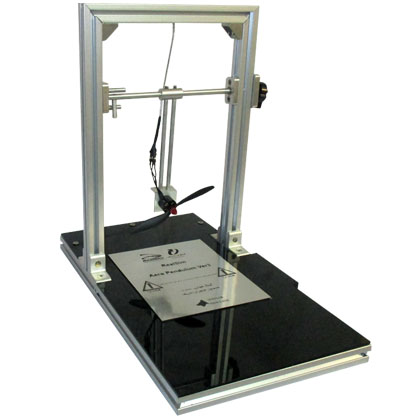
\includegraphics[width=8cm]{obr/pendulum.jpg}}
	\hfill
	\subfigure[{Aeropendulum univerzity Arizona\cite{enikov_campa_2012}.}]{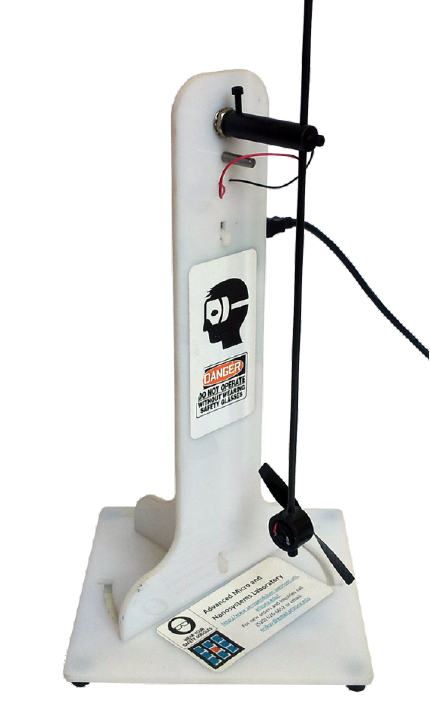
\includegraphics[width=6.5cm]{obr/arizona.png}}
	\hfill
	\caption{Experimentálne moduly vzdušného kyvadla.}\label{OBRAZOK 1.2}
\end{figure}

\newpage
Open-source\footnote[1]{Open-source je zo všeobecného pohľadu akákoľvek informácia, ktorá je dostupná verejnosti bez poplatku(s voľným prístupom), s ohľadom na fakt, že jej voľné šírenie zostane zachované.} projekt AutomationShield je zameraný na vývoj hardvérových a softvérových nástrojov, určených na vzdelávanie a doplnenie vzdelávacieho procesu. Jadrom celého projektu je tvorba rozširujúcich dosiek (shieldov) vyvíjaných pre populárny typ prototypizačných dosiek s mikrokontrolérmi Arduino. Tieto pomerne lacné učebné pomôcky majú za cieľ skvalitniť výučbu strojného inžinierstva, mechatroniky a základov automatického riadenia\cite{Auto}.

Všetky informácie ohľadom projektu AutomationShield, sú dostupné na open-source platforme GitHub\cite{Git}, ktorá slúži ako knižnica kódov, návodov a postupov, ktoré sú voľne dostupné na čítanie a úpravu. Na samostatnej stránke AutomationShieldu nájdeme zoznam jednotlivých shieldov a to, v akom procese výroby a fungovania sa nachádzajú. Ku každému shieldu nájdeme jeho podrobnú dokumentáciu, knižnice, zdrojové kódy, ako aj predprogramované ukážky jeho fungovania. 

Hlavnou motiváciou tohoto projektu je nízka dostupnosť a vysoká cena podobných učebných pomôcok. Z môjho pohľadu je výučba častokrát až príliš zameraná na memorovanie faktov a teórie, namiesto praktických experimentov a skúseností typu pokus-omyl. Študenti pochopia vyučovanú teóriu jednoduchšie, pokiaľ majú možnosť experimenty sami tvoriť, skúmať a testovať\cite{Dhanapal2013ASO}. 

V roku 2005 prišla na trh prototypizačná doska Arduino. Projekt vznikal v Taliansku ako kolaborácia medzi viacerými nadšencami elektrotechniky a programovania, na ktorej čele bol Massimo Banzi. Veľkou výhodou dosiek Arduino a ich nadstavbových shieldov je fakt, že sú pomerne lacné a majú malé rozmery (Arduino UNO: 68.6$\times$53.4mm\cite{UNO}). Tieto skutočnosti umožňujú študentom pracovať na experimentoch nielen na pôde školy, ale experimenty si môžu zobrať aj domov. 

\begin{figure}[!tbh]
	\centering
	\includegraphics[width=80mm]{obr/arduino.jpg}
	\caption{{Arduino UNO R3\cite{UNOFOTO}.}}\label{OBRAZOK 1.3}
\end{figure}

Na fungovanie a programovanie dosky postačuje len USB kábel, programovací softvér a samotná doska. Vzhľadom na nízky počet potrebných komponentov a fakt, že mikročip Arduina je v prípade poruchy jednoducho vymeniteľný\footnote[2]{Platí pri mikročipoch typu DIP(Dual in-line package), ktoré stačí jednoducho vytiahnuť z konektora bez použitia spájkovania.}, je jeho používanie na školách príjemné a jednoduché. Mikrokontroléri Arduino využívame z dôvodu nízkej ceny, širokej dostupnosti rôznych modelov, postačujúcej výpočtovej sile a príjemnému používateľskému rozhraniu. Pre naše účely využívame najmä dve verzie Arduina. Prvou z nich je doska Arduino UNO R3  obr.\ref{OBRAZOK 1.3}. Na doske sa nachádza 14 digitálnych a 6 analógových pinov.

Na prácu v MATLABE a Simulinku využívame najmä Arduino Mega 2560 R3 obr.\ref{OBRAZOK 1.32}. Na tejto doske sa nachádza 54 digitálnych a 16 analógových pinov. AeroShield je kompatibilný so všetkými doskami s označením R3 alebo s doskami, ktoré majú rozloženie pinov rovnaké ako Arduino UNO R3. 

Niektoré piny sú označené špeciálnym symbolom ,,$\sim$''. Tieto piny sú schopné generovať PWM\footnote[3]{Šírková modulácia impulzov alebo PWM je technika na dosiahnutie analógových výsledkov pomocou digitálnych prostriedkov a to za pomoci striedania dĺžok medzi High a Low stavom, resp. zapnutý a vypnutý stav.} signál, ktorý využívame na ovládanie motora kyvadla.

\begin{figure}[!tbh]
	\centering
	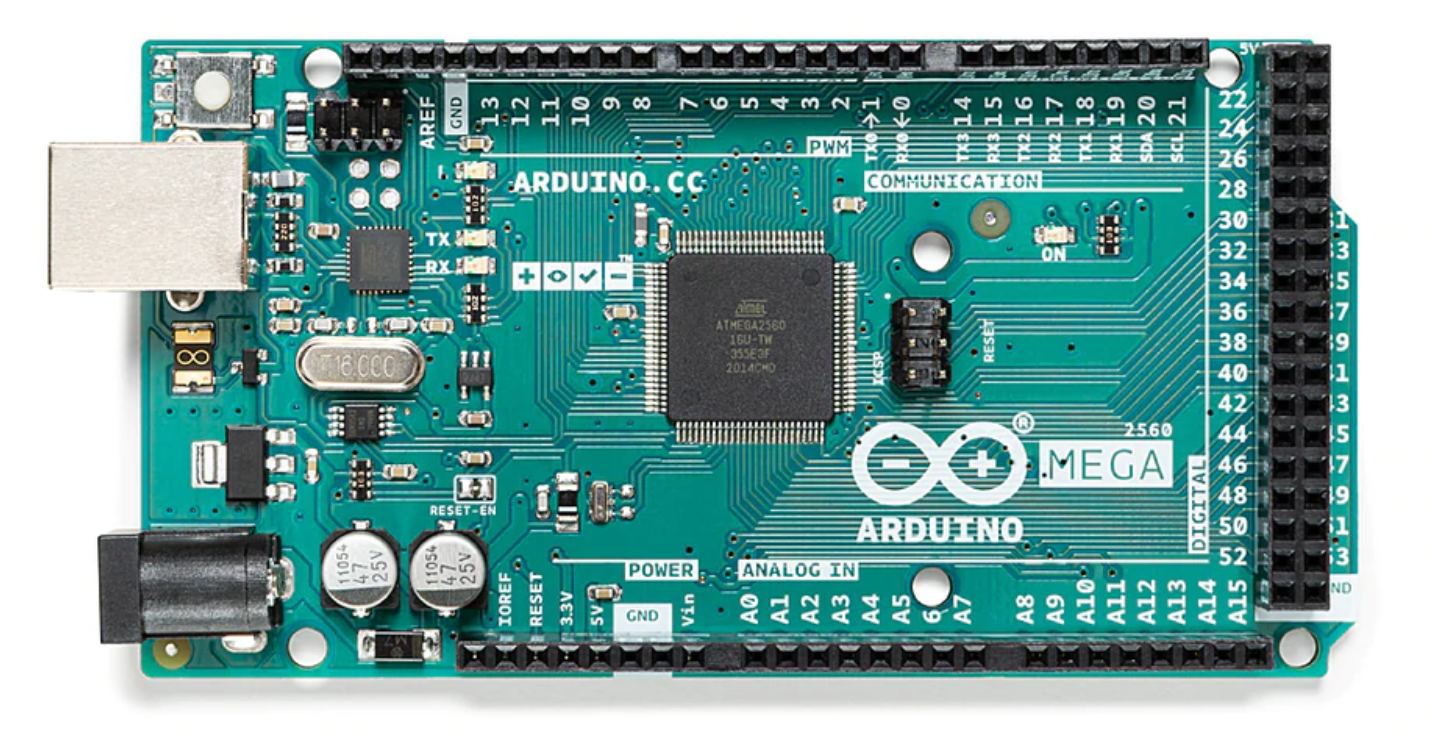
\includegraphics[width=100mm]{obr/mega.png}
	\caption{{Arduino Mega 2560 R3\cite{megafoto}.}}\label{OBRAZOK 1.32}
\end{figure}

\newpage
Práca je rozdelená na štyri logické celky. Na začiatku v časti hardvér je opísaný základný princíp fungovania shieldu a jeho jednotlivé súčiastky. V tejto časti sa taktiež opisuje tvorba schémy zapojenia a dosky plošných spojov AeroShieldu. 

V softvérovej časti sú bližšie predstavené spôsoby programovania shieldu. Opisuje sa tu tvorba knižníc jednotlivých programov, v ktorých sú tvorené didaktické príklady pre AeroShield.

Predposlednú časť práce tvoria samotné didaktické príklady, za ktorými nasleduje záverečná časť, ktorou je finálne zhodnotenie práce.





\chapter{AeroShield}

Práca je založená na už započatom projekte vzdušného kyvadla. Na jeho tvorbe sa najviac podieľali študenti: Dávid Vereš, Ján Boldocký, Tadeas Vojtko a Denis Skokan. Prvá verzia dosky a samotného kyvadla, vznikla ako záverečný projekt na predmet Mikropočítače a mikroprocesorová technika. Fotografiu zostavenej dosky, môžeme vidieť na obr.\ref{OBRAZOK 2.1.1}.


\begin{figure}[tbh]
	\centering
	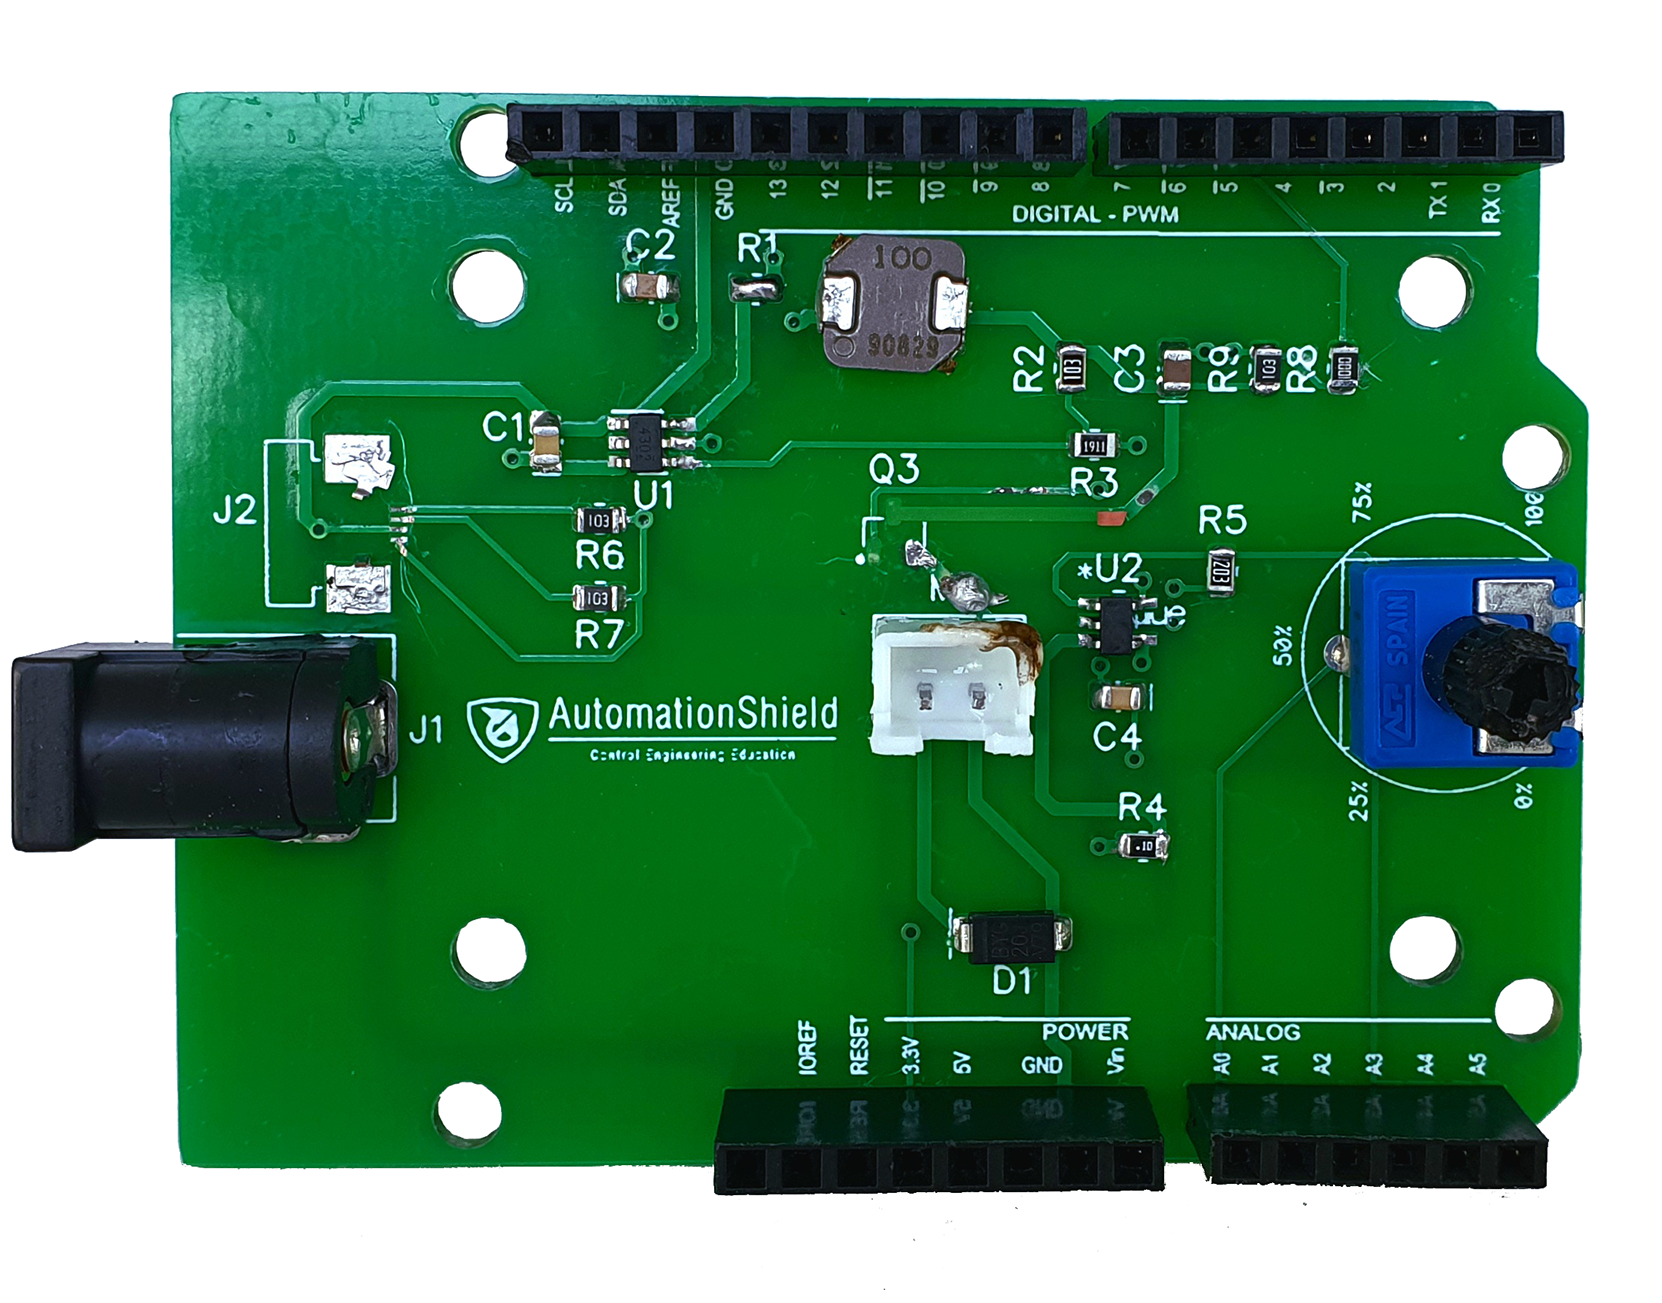
\includegraphics[width=80mm]{obr/oldshield.jpg}
	\caption{Prvá verzia AeroShieldu. }\label{OBRAZOK 2.1.1}
\end{figure}


V novej verzii dosky bolo odstránených niekoľko nedostatkov predchádzajúcej verzie. Jednalo sa o:

\begin{itemize}
	\item neprepojenie pinov komunikácie I2C tj. piny SDA a SCL senzoru hall efektu, ktorý slúži na meranie uhlu natočenia kyvadla,
	\item nesprávne zapojenie mosfetu PMW45EN, ktorý ovláda PWM signál idúci do akčného člena,
	\item nesprávne umiestnená ochranná dióda na konektoroch akčného člena,
	\item nesprávne zapojený obvod s čipom INA169, ktorý slúži na meranie prúdu,
	\item neprepojenie nulového konektora shieldu s nulovým konektorom arduina.
\end{itemize}

Základom tejto bakalárskej práce teda bolo pochopiť jednotlivé časti zapojenia, analyzovať chyby a ich následná oprava. V rámci projektu bola vytvorená hlavná doska, na ktorej sa nachádza väčšina elektroniky a menšia doska tzv. breakout board obr.\ref{OBRAZOK 2.1.2}.b, ktorý je uchytený v hornej časti kyvadla a slúži na fungovanie senzoru hall efektu. Táto doska fungovala bezproblémovo a teda nebolo potrebné nijakým spôsobom meniť jej schému zapojenia obr.\ref{OBRAZOK 2.1.2}.a. Breakout boardu sa budeme bližšie venovať v časti \ref{PCBcka}.

\begin{figure}[!tbh]
	\hfill
	\subfigure[Schéma zapojenia breakout boardu.]{\includegraphics[width=10cm]{obr/as5600.png}}
	\hfill
	\subfigure[Breakout board.]{\includegraphics[width=5cm]{obr/fotoBreak.png}}
	\hfill
	\caption{Meranie uhla kyvadla}\label{OBRAZOK 2.1.2}
\end{figure}


\newpage
\section{Hardvér}
\subsection{Popis súčiastok}

V tejto časti sa bližšie pozrieme na jednotlivé súčasti zapojenia AeroShieldu. Konkrétne sa jedná o tieto prvky:
\begin{multicols}{2}
	\begin{itemize}
		\item napájanie
		\item ovládanie akčného člena
		\item meranie uhla natočenia kyvadla
		\item meranie prúdu
	\end{itemize}
\end{multicols}


\subsubsection{Znižovací menič}
\label{nap}

Na napájanie akčného člena, motorčeka, potrebujeme napätie v rozmedzí 0-3,7V. Na shield je však privádzané, pomocou koaxiálneho napájacieho konektora, napätie 12V, ktoré by mohlo motor pri dlhšom používaní zničiť. Na zníženie napätia preto použijeme znižovací menič tzv. buck converter. 

Hlavnou časťou konvertora je čip TPS56339 od výrobcu Texas Instruments obr.\ref{OBRAZOK 2.1}.b. Znižovanie napätia funguje za pomoci dvoch integrovaných N-kanálových 70-m$\Omega$ a 35-m$\Omega$ high-side mosfetov\footnote[4]{N-kanálový mosfet je typ mosfetu, v ktorom tok prúdu nastáva kvôli pohybujúcim sa, záporne nabitým elektrónom. $"High-side"$ znamená, že prúd prechádza z napájania, cez mosfet, do záťaže a potom do zeme.}, v spolupráci s ďalšími komponentami. Celkový prevádzkový prúd zariadenia je približne 98$\upmu$A, keď funguje bez spínania a bez záťaže. Keď je zariadenie vypnuté, napájací prúd je približne 3$\upmu$A a zariadenie umožňuje nepretržitý výstupný prúd do 3 A\cite{buckobr}.

\begin{figure}[!tbh]
	\hfill
	\subfigure[Schéma zapojenia znižovacieho meniča.]{\includegraphics[width=9cm]{obr/schemaBuck.png}}
	\hfill
	\subfigure[{čip TPS56339.\cite{buckobr}}]{\includegraphics[width=5cm]{obr/cip.eps}}
	\hfill
	\caption{buck converter}\label{OBRAZOK 2.1}
\end{figure}

Na čip je privádzané napätie 12V ktoré sa pomocou zapojenia viditeľného na schéme obr.\ref{OBRAZOK 2.1}.a, znižuje na napätie 3,7V. Domnievali sme sa že napájanie motora musí byť realizované externe, pomocou koaxiálneho napájacieho konektora z dôvodu vysokého prúdu odoberaného motorom počas silného zaťaženia. Rovnaký konektor sa síce nachádza aj na doske Arduino UNO a pomocou VIN pinu sa z neho dajú napájať napätím 6-12V aj iné zariadenia, avšak tento pin je napojený na diódu, obmedzujúcu prúd na 1A\cite{ampere}\cite{ampere2}. 

Pri testovaní prototypov druhej verzie AeroShieldu, sa merané hodnoty prúdu pohybovali nad hodnotu 1A, čo by zničilo spomínanú internú diódu na doske Arduino UNO. 
Po zostavení druhej verzie shieldu a opätovnom meraní odoberaného prúdu, bola maximálna dosahovaná hodnota menšia ako 0,5A. Z tohoto dôvodu sme sa rozhodli pre zmenu v schéme kyvadla z ktorej sme odobrali externý napájací konektora následne bola vyrobená nová doska plošných spojov. Tretej verzii AeroShieldu sa bližšie venujeme v časti...

\subsubsection{Akčný člen}
\label{akcclen}

Ako akčný člen AeroShieldu je použitý 7mm, 3,7V motorček na jednosmerný prúd bez jadra, používaný hlavne pre pohon dronov. “Coreless motor“, alebo motor bez jadra, je motor s cievkou navinutou samou na sebe a nie na železe\cite{coreless}. Stator je vyrobený z magnetov na báze vzácnych zemín, ako je neodým alebo SmCo(samárium-kobalt).

Takýto motor ponúka mnoho výhod oproti motoru so železným jadrom. Tým že jadro v sebe nemá železo, výrazne sa znižuje hmotnosť a tým aj zotrvačnosť rotora, čo je dôležité pre naše použitie, kedy potrebujeme dosahovať vysokú akceleráciu a rýchle spomalenie rotora. Ďalšou výhodou je fakt, že nedochádza k stratám na železe a tým pádom sa účinnosť takýchto motorov blíži až ku 90\%\cite{5545147}. Motor, resp. otáčky motora sú riadené pomocou PWM signálu a ten do motoru prechádza cez N-kanálový mosfet PMV45EN2 od výrobcu Nexperia\cite{pmv}.


\begin{figure}[!tbh]
	\hfill
	\subfigure[Schéma zapojenia motorčeka.]{\includegraphics[width=7cm]{obr/MotorScheme.png}}
	\hfill
	\subfigure[{Akčný člen sústavy.\cite{corelessMotor}}]{\includegraphics[width=7cm]{obr/coreless.jpg}}
	\hfill
	\caption{Zapojenie akčného člena a typ motorčeka}\label{OBRAZOK 2.3}
\end{figure}


\subsubsection{Meranie prúdu}
\label{merprud}

Z dôvodu merania prúdu odoberaného motorom, bol do schémy pridaný monitor prúdu, takzvaný "current shunt monitor". Nameraný prúd môžeme využiť na implementácie riadenia motora na základe prúdu, ktorý odoberá. AeroShield používa snímač INA169NA/250 od výrobcu Texas Instruments obr.\ref{OBRAZOK 2.3.2}.b.

INA169 funguje na základe zaznamenávania zmien napätia na stranách shunt rezistora obr.\ref{OBRAZOK 2.3.2}.a. Na základe nameraného úbytku napätia, vysiela senzor podľa nami zvoleného stupňa zosilnenia, prúd ktorý je ďalej pomocou rezistoru $R_{l}$ premenený na napätie s maximálnou hodnotou $V_{OUTMAX} = V_{IN-} - 0.5V $.

Prúd $I_{s}$ odoberaný motorom, vypočítame pomocou vzorca $I_{s} = {(V_{OUT}\: x \: 1k\Omega)}$/${(R_{s} \: x \: R_{l})}$ kde $V_{OUT}$ je napätie namerané na výstupe, 1k$\Omega$ je konštanta vnútorných odporov senzoru, $R_{s}$ je hodnota shunt rezistora v $\Omega$ a $R_{l}$ je hodnota rezistora na výstupe, taktiež v $\Omega$\cite{INA}.

\begin{figure}[!tbh]
	\hfill
	\subfigure[Schéma zapojenia snímača prúdu.]{\includegraphics[width=9cm]{obr/INAschema.png}}
	\hfill
	\subfigure[{Senzor INA169NA/250\cite{INAobr}}]{\includegraphics[width=6cm]{obr/ina.png}}
	\hfill
	\caption{meranie prúdu}\label{OBRAZOK 2.3.2}
\end{figure}





\subsubsection{Meranie uhla kyvadla}
\label{meruhl}

Na fungovanie AeroShieldu je dôležité vedieť s vysokou presnosťou merať uhol naklonenia kyvadla. Na tento účel sme si zvolili meranie uhlu bezkontaktnou formou, pomocou snímača hall efektu. Hallov jav vieme opísať ako vznik priečneho elektrického poľa v pevnom materiáli, keď ním preteká elektrický prúd a tento materiál je umiestnený v magnetickom poli, ktoré je kolmé na prúd\cite{Hall}. Toto elektrické pole resp. vznik elektrického potenciálu vieme detegovať ako Hallovo napätie a na základe jeho zmeny, vieme určiť rotáciu kyvadla. Fyzikálna podstata tohoto javu je na obr.\ref{OBRAZOK 1.323}, kde V$_H$ je Hallovo napätie, B je magnetické pole, F$_m$ magnetická sila pôsobiaca na negatívne prenášače náboja, F$_e$ elektrická sila z nahromadeného náboja, I je dohodnutý smer elektrického prúdu. 

\begin{figure}[!tbh]
	\centering
	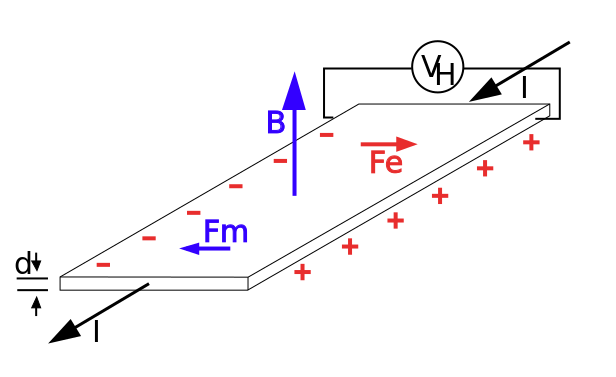
\includegraphics[width=100mm]{obr/hallovjav.png}
	\caption{Schematická reprezentácia hallovho javu.}\label{OBRAZOK 1.323}
\end{figure}

V kyvadle je na konci horizontálneho ramena umiestnený špeciálny magnet kruhového tvaru, ktorý je polarizovaný naprieč prierezom magnetu. Ako senzor na meranie hall efektu je použitý AS5600 od výrobcu OSRAM obr.\ref{OBRAZOK 2.2}.b. Signály prichádzajúce zo snímača sa najprv zosilnia, následne sú filtrované a prechádzajú konverziou pomocou analógovo-digitálneho prevodníka(ADC). Snímaná je aj intenzita magnetického poľa, ktorou senzor pomocou
automatického riadenia zosilnenia(AGC), kompenzuje zmeny teploty priestoru a taktiež zmeny sily magnetického poľa.

Na výber sú dva typy výstupu a to analógový výstup alebo digitálny výstup s kódovaním PWM. Senzor má taktiež možnosti interného programovania pomocou rozhrania I2C.
V našom prípade používame 12-bitový analógový výstup s rozlíšením 0°5'16". Toto rozlíšenie nám umožňuje s vysokou presnosťou kontrolovať naklonenie kyvadla a na základe získaných informácii ovplyvňovať fungovanie akčného členu sústavy. Schéma zapojenia čipu na meranie uhlu môžeme vidieť na obr.\ref{OBRAZOK 2.2}.a.



\begin{figure}[!tbh]
	\hfill
	\subfigure[Schéma zapojenia čipu na meranie uhlu.]{\includegraphics[width=10cm]{obr/as5600.png}}
	\hfill
	\subfigure[{čip AS5600\cite{As5600obr}}]{\includegraphics[width=4cm]{obr/hall.jpg}}
	\hfill
	\caption{meranie uhla kyvadla}\label{OBRAZOK 2.2}
\end{figure}

\newpage


\subsection{Schéma zapojenia}

Všetky schémy zapojenia boli tvorené v bezplatnej verzii programu DipTrace. DipTrace slúži ako prostredie na tvorbu elektrotechnických schém a dosiek plošných spojov. Program v sebe zahŕňa aj časť pre tvorbu jednotlivých komponentov, pokiaľ sa tieto už nenachádzajú v niektorej z knižníc programu.

Nie všetky komponenty potrebné na tvorbu schémy zapojenia boli zahrnuté v knižniciach DipTracu, avšak tieto komponenty sú dostupné na stránkach výrobcov, odkiaľ sa dajú stiahnuť a následne použiť v schéme\cite{AS5600Downl}\cite{TPS56339Downl}\cite{INAobr}. Do programu bola taktiež vložená knižnica AutomationShieldu ktorá má v sebe najčastejšie používané komponenty. Pri tvorbe schémy zapojenia sa najskôr všetky potrebné komponenty umiestnia na štvorčekovú plochu a približne sa určí ích poloha. Jednotlivé komponenty majú podobu elektrotechnických značiek a každý komponent má ku sebe priradené reálne vlastnosti daného dielu(veľkosť, zapojenie, dĺžka pinov a iné).

Polohu volíme takú, aby schéma bola čo najprehľadnejšia a komponenty ktoré sú medzi sebou prepojené, boli čo najbližšie pri sebe. Akonáhle máme všetky komponenty uložené začneme s ich postupným prepájaním. Pri zapájaní jednotlivých komponentov sa riadime katalógovými listami jednotlivých komponentov, v ktorých býva zväčša aj návrh ich zapojenia.

DipTrace umožňuje rozdielne zafarbovanie jednotlivých elektrických spojení, rozličnými farbami a názvami obr.\ref{OBRAZOK 2.3.5}. Tento fakt nám veľmi uľahčuje na prvý pohľad rozoznať napríklad elektrické spojenia zeme- 0V zelená, fázové spojenia- 3,3V červená. Na schéme zapojenia sú použité nasledujúce komponenty:
\begin{multicols}{3}
	\begin{itemize}
		\item R- Rezistor
		\item C- Kapacitor
		\item J- Konektor
		\item U- Mikročip
		\item L- Cievka
		\item D- Dióda
		\item M- Motor
	\end{itemize}
\end{multicols}


\begin{figure}[!tbh]
	\includegraphics[width=\textwidth]{obr/aeroSchema.png}
	\caption{Schéma zapojenia AeroShieldu.}\label{OBRAZOK 2.3.5}
\end{figure}

\subsection{Doska plošných spojov}
\label{PCBcka}

Po návrhu a kontrole schém zapojenia sa schémy ďalej spracovávajú do podoby dosky plošných spojov. Schémy exportujeme do programu DipTrace PCB v ktorom máme následne niekoľko možností postupu. Jednotlivé komponenty sa nám už zobrazujú v reálnej podobe, takže vidíme ich veľkosť a rozmiestnenie konektorov na spájkovanie. Dosky plošných spojov majú niekoľko výhod, ale aj negatív oproti ponúkaným alternatívam\cite{dosky}. 

Výhodou je fakt, že vodivé spojenia medzi jednotlivými súčiastkami sú narozdiel od typických káblových spojení, realizované vrstvou medi, ktorá je ukrytá pod ochrannými vrstvami dosky. Ďalšou z výhod dosiek plošných spojov je skutočnosť, že sú odolné a kompaktné\cite{PCBlife}. Tým že vodivé cesty môžu mať veľmi malé rozmery, ovplyvňujúcim faktorom veľkosti dosky plošných spojov je samotná veľkosť použitých komponentov. 

Hotová schéma zapojenia je prenesená do programu DipTrace PCB. Program ponúka možnosť automatického alebo manuálneho rozmiestnenia komponentov.

\begin{figure}[!tbh]
	\hfill
	\subfigure[Vrchná strana breakout boardu]{\includegraphics[width=7cm]{obr/breakoutTOP.png}}
	\hfill
	\subfigure[Spodná strana breakout boardu]{\includegraphics[width=7cm]{obr/breakoutbottom.png}}
	\hfill
	\caption{Vedľajšia doska AeroShieldu- breakout board.}\label{OBRAZOK 2.6}
\end{figure}

Po zvolení optimálneho rozmiestnenia komponentov treba jednotlivé piny poprepájať vodivými cestami, ktoré nám nahrádzajú funkciu káblov. Máme možnosť zvoliť automatické rozmiestnenie ciest alebo ich manuálnu tvorbu. Ako je vidieť na obr.\ref{OBRAZOK 2.4}.a, nie všetky cesty majú rovnakú šírku. Dôvodom je fakt že niektorými cestami tečie vyšší prúd. V zásade sa používa pravidlo, čím vyšší prúd preteká vodičom, tým väčšiu plochu prierezu by mal mať. Prúdy pretekajúci vodičom tento vodič zahrieva. Pokiaľ je toto zahrievanie nadmerné, môže dôjsť k poškodeniu vodiča.  

Tvorba elektrických ciest má niekoľko pravidiel. Najdôležitejšie z nich je, že cesty spájajúce rozdielne vodiče sa nemôžu križovať. Pokiaľ by k takémuto kríženiu došlo, jednotlivé cesty sa vzájomne vyskratujú. Z toho dôvodu treba niekedy cestu priviesť na druhú stranu dosky plošných spojov kde v jej pokračovaní neprekáža iná cesta. Na tento účel sa používajú vodivé diery "via", spájajúce obe strany dosky. Druhá verzia dosky AeroShieldu je na obr.\ref{OBRAZOK 2.4}. 



\begin{figure}[!tbh]
	\centering
	\includegraphics[width=8cm]{obr/AeroShieldTOP.png}
	
	(a)
	
	\includegraphics[width=8.5cm]{obr/AeroShieldBOTTOM.png}
	
	(b)
	
	\caption{(a) Vrchná strana AeroShieldu. (b) Spodná strana AeroShieldu.}
	\label{OBRAZOK 2.4}
\end{figure}



Po finálnej kontrole zapojenia komponentov na doske plošných spojov, môžeme tieto dosky uložiť do formátu gerber. Súbory typu gerber v sebe ukladajú presné zloženie finálnej dosky plošných spojov a to po jej jednotlivých vrstvách. Zkonvertované súbory zasielame výrobcovi PCB dosiek kde si môžeme zvoliť parametre dosky ako jej farbu, typy spájkovacích doštičiek a iné. Podobu finálnej dosky AeroShieldu môžeme vidieť na obr.\ref{OBRAZOK 2.7}.a a dosky breakout boardu na obr.\ref{OBRAZOK 2.7}.b.


\begin{figure}
	\hfill
	\subfigure[Hlavná doska AeroShieldu]{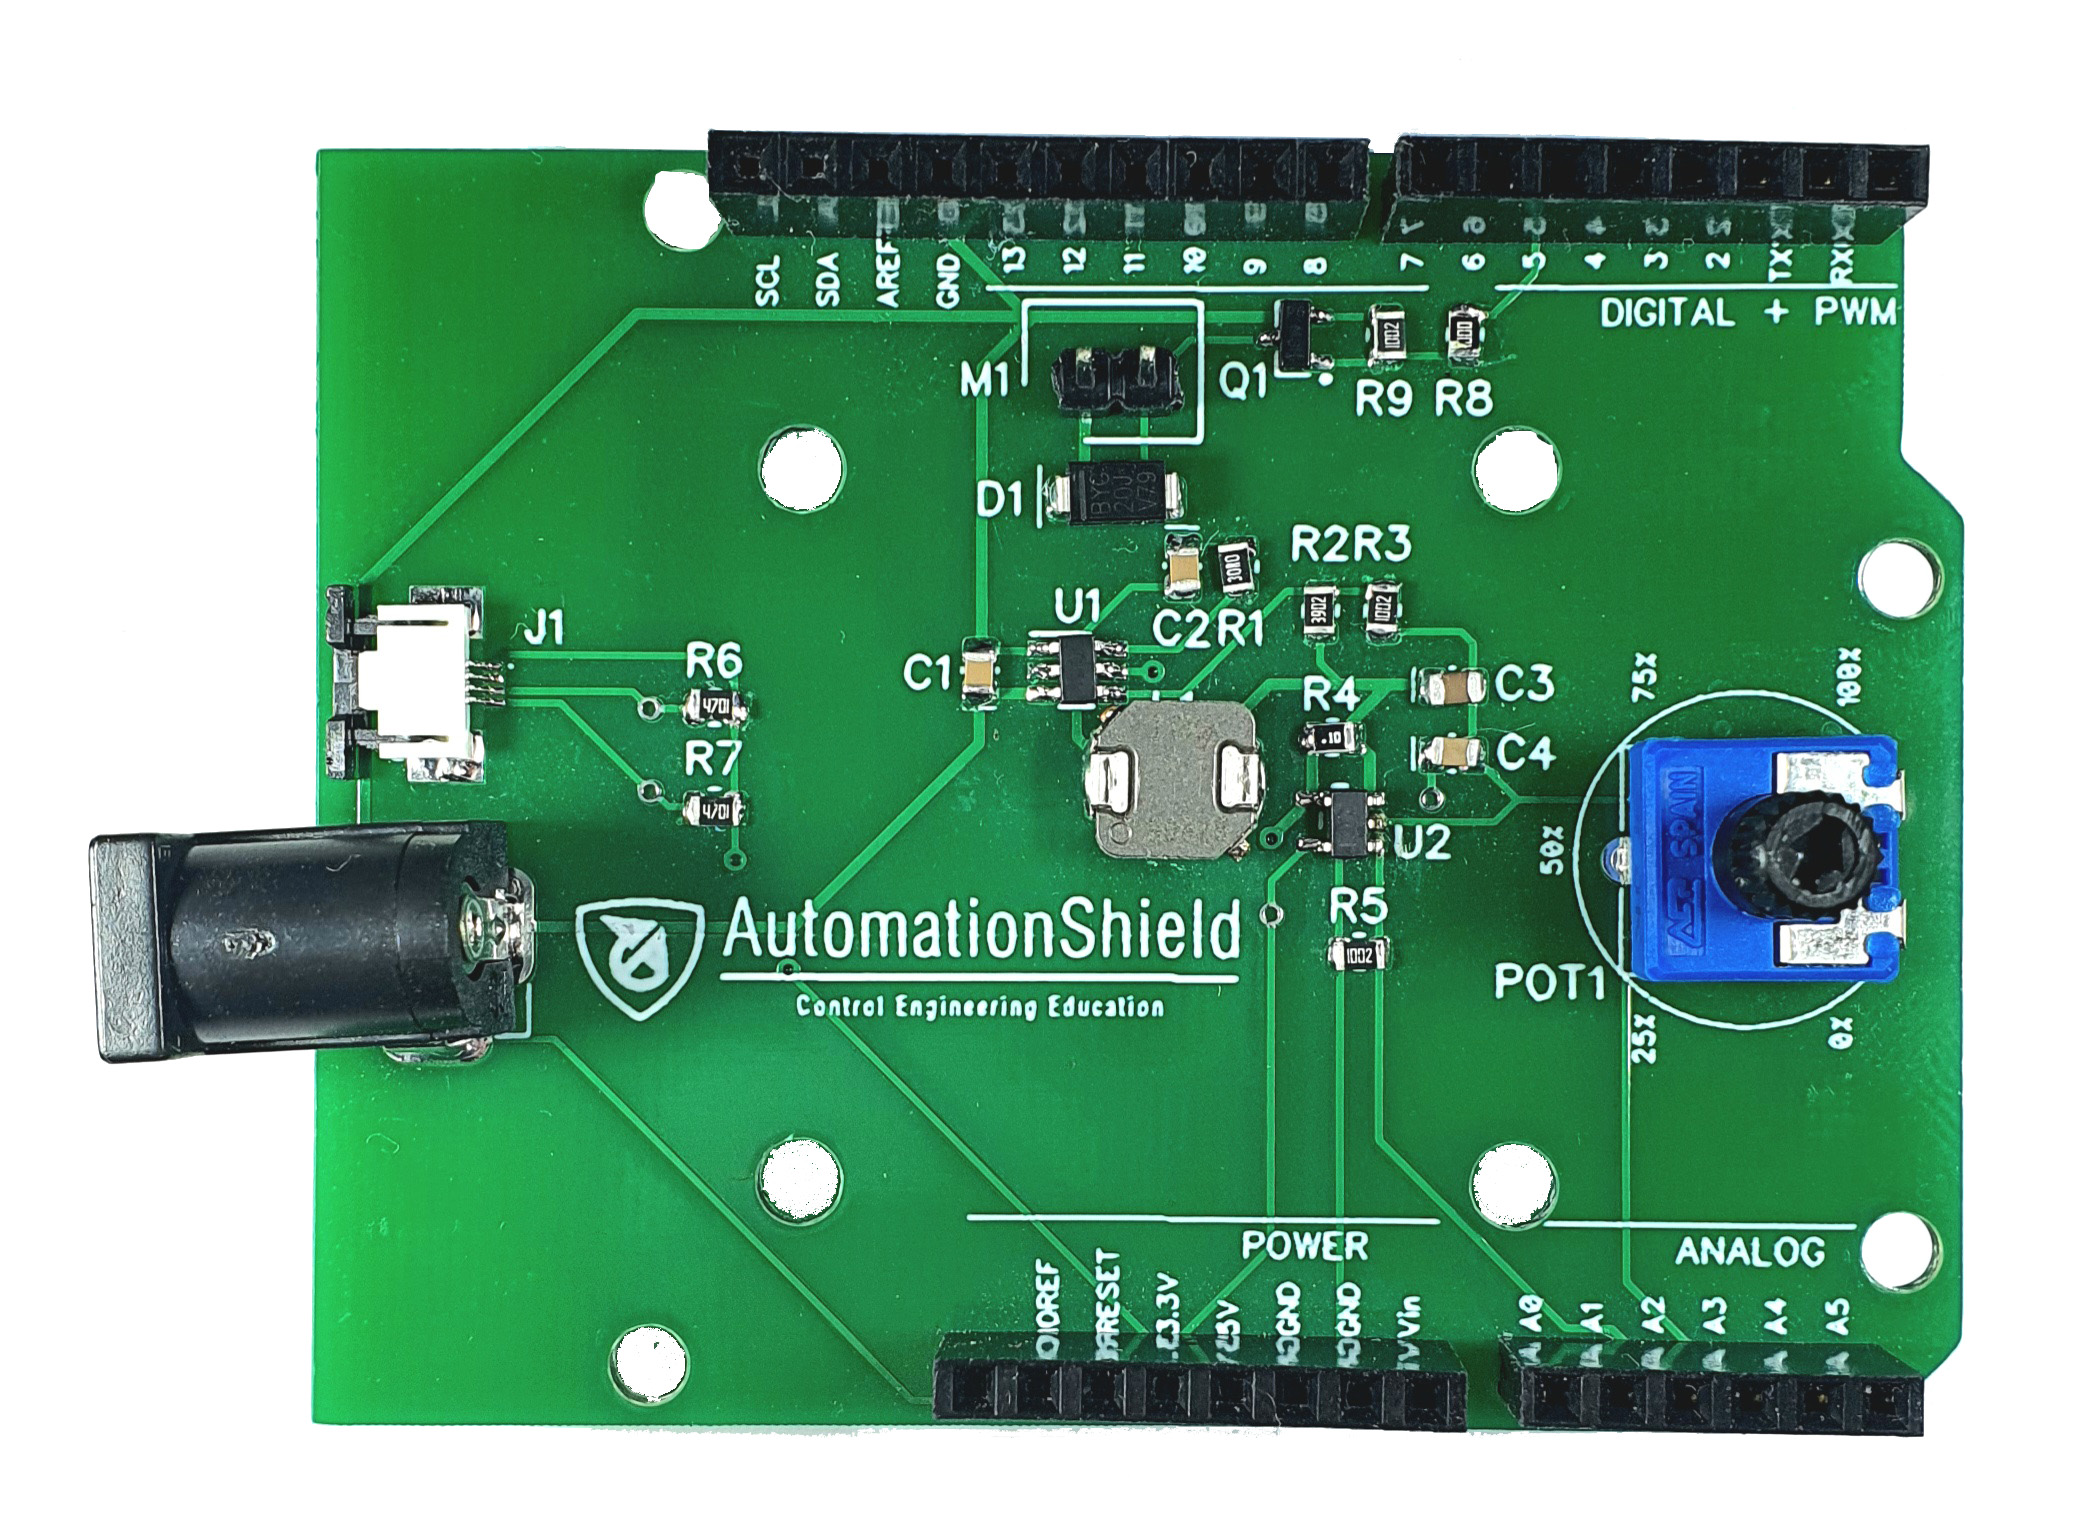
\includegraphics[width=9cm]{obr/AeroShield.jpg}}
	\hfill
	\subfigure[Vedľajšia doska AeroShieldu]{\includegraphics[width=6cm]{obr/fotoBreak.png}}
	\hfill
	\caption{Dosky plošných spojov AeroShieldu.}\label{OBRAZOK 2.7}
\end{figure}

\subsection{Model držiaku kyvadla}

Telo kyvadla ako aj všetky konektory spájajúce jeho jednotlivé časti, boli vytvorené v 3D modelovacom softvéri CATIA obr.\ref{OBRAZOK 1.1}. Zámerom bolo vytvoriť pevný a zároveň estetický držiak, ktorý sa dá následne vytlačiť na 3D tlačiarni. Telo kyvadla stojí na štyroch nožičkách, ktoré sú priskrutkované k hlavnej doske plošných spojov. Stred kyvadla je dutý, a sú nim vedené káble napájania motorčeka. V hornej časti držiaku sa nachádzajú diery na priskrutkovanie breakout boardu. 

\begin{figure}
	\centering
	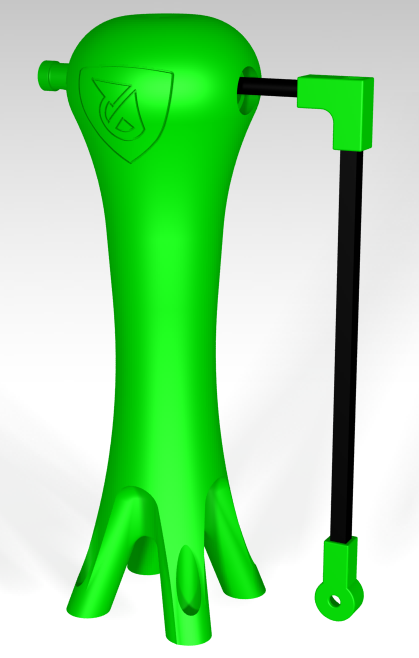
\includegraphics[width=80mm]{obr/AeroCatiaa.png}
	\caption{Model kyvadla, tvorený v programe CATIA.}\label{OBRAZOK 1.1}
\end{figure}

\subsection{Cenová kalkulácia AeroShieldu}

Hlavnou podmienku pri tvorbe AeroShieldu, bola jeho funkcionalita, no zároveň nízka cena. Za účelom predstavy cenovej relácie jedného kusu AeroShieldu, bola zostavená tabuľka\ref{Cenova kalkulacia} s použitými komponentami, ich počtom a reálnou kúpnou cenou v eurách(spolu s DPH). Pri komponentoch ako sú rezistory a kapacitory, bola cena určená ako priemerná hodnota týchto komponentov pri kúpe viac ako 100kusov, keďže pri kúpe zopár kusov(1-20) je ich cena rádovo vyššia, ako cena pri nákupoch viacero kusov. 

\begin{table}
	\begin{tabular}{p{0.25\textwidth} p{0.43\textwidth} p{0.05\textwidth} p{0.07\textwidth} p{0.07\textwidth}}
		\hline
		\multicolumn{1}{|l}{\textbf{Názov}} & \textbf{Popis}                                     & \multicolumn{1}{l}{\textbf{Ks.}} & \multicolumn{1}{l}{\textbf{Cena v \euro}} & \multicolumn{1}{l|}{\textbf{Spolu}} \\ \hline
		Kapacitor                           & SMD, sot23                                         & 6                                  & 0,08                                      & 0,48                                        \\
		Dióda                               & 1N400IG                                            & 1                                  & 0,1                                      & 0,1                                        \\
		FFC konektor                        & FFC 4pin                                           & 2                                  & 0,2                                      & 0,4                                        \\
		Cievka                              & IND1210                                            & 1                                  & 0,2                                      & 0,2                                        \\
		Konektor DC motora                  & JST-XH 2,54                                        & 1                                  & 0,4                                      & 0,4                                        \\
		Motor                               & Howellp 7x20mm Motor                               & 1                                  & 2,1                                      & 2,1                                        \\
		Potenciometer                       & CA14                                               & 1                                  & 0,45                                     & 0,45                                       \\
		Mosfet                              & pmv45en2                                           & 1                                  & 0,04                                     & 0,04                                       \\
		Rezistor                            & SMD, sot23                                         & 9                                  & 0,08                                      & 0,72                                        \\
		Buck converter                      & TPS56339                                           & 1                                  & 2,78                                     & 2,78                                       \\
		Shunt monitor                       & INA169/NA                                          & 1                                  & 0,98                                     & 0,98                                       \\
		Hall senzor                         & AS5600                                             & 1                                  & 1,48                                     & 1,48                                       \\
		3D komponenty                       & model kyvadla a spojovacie prvky                   & 4                                  & 2,2                                      & 2,2                                        \\
		Gulôčkové ložiská                   & BB-694-B180-30-ES IGUS                             & 2                                  & 2,75                                     & 5,5                                        \\
		Prepájacie káble FFC                & akékoľvek 4 pin, dĺžka min 15cm                    & 1                                  & 0,52                                     & 0,52                                       \\
		Prepajací kábel motor               & akékoľvek, dĺžka min 35cm                          & 1                                  & 0,3                                      & 0,3                                        \\
		Šróby                               & 4x M3x40 4x M4x15                                  & 8                                  & 0,25                                     & 2                                          \\
		Karbónové trubičky                  & 1x kruhový prierez 10cm, 1x štvorcový prierez 10cm & 2                                  & 1,9                                      & 3,8                                        \\
		PCB shield                          & Výroba JLCPCB                                      & 1                                  & 0,35                                     & 0,35                                       \\
		PCB brakout                         & Výroba JLCPCB                                      & 1                                  & 0,35                                     & 0,35                                       \\
		Matice                              & M4                                                 & 4                                  & 0,2                                      & 0,8                                        \\ \hline
		\multicolumn{1}{|l}{}               &                                                    & \multicolumn{1}{l}{}               & \textbf{Spolu}                           & \multicolumn{1}{c|}{\textbf{25,95\euro}}        \\ \hline
	\end{tabular}
\caption{Cenová kalkulácia AeroShieldu.}
\label{Cenova kalkulacia}
\end{table}

\subsection{Tretia verzia AeroShieldu}

V tretej verzii AeroShieldu obr.\ref{OBRAZOK 2.8}, bol odstránený napájací konektor a napájanie je realizované z konektora, ktorý sa nachádza na doske Arduino. Na Shield je napätie 12V privádzané pomocou \verb|vin| pinu obr.\ref{OBRAZOK 2.9}. Prúd odoberaný motorom nedosahuje hodnoty väčšie ako 1A a teda takéto napájanie je bezpečné a nehrozí pri ňom poškodenie hardvéru Arduina. Ďalej bolo upravené rozloženie niektorých komponentov. Jedná sa hlavne o konektor \verb|J1|, spájajúci hlavnú dosku s breakout doskou, rezistory \verb|R8 a R9| a mosfet \verb|Q1|. Ako posledná úprava bola otočená polarity potenciometra, ktorý bol na druhej verzii AeroShieldu pripojený opačne, ako značil popis na doske. 

\begin{figure}[!tbh]
	\centering
	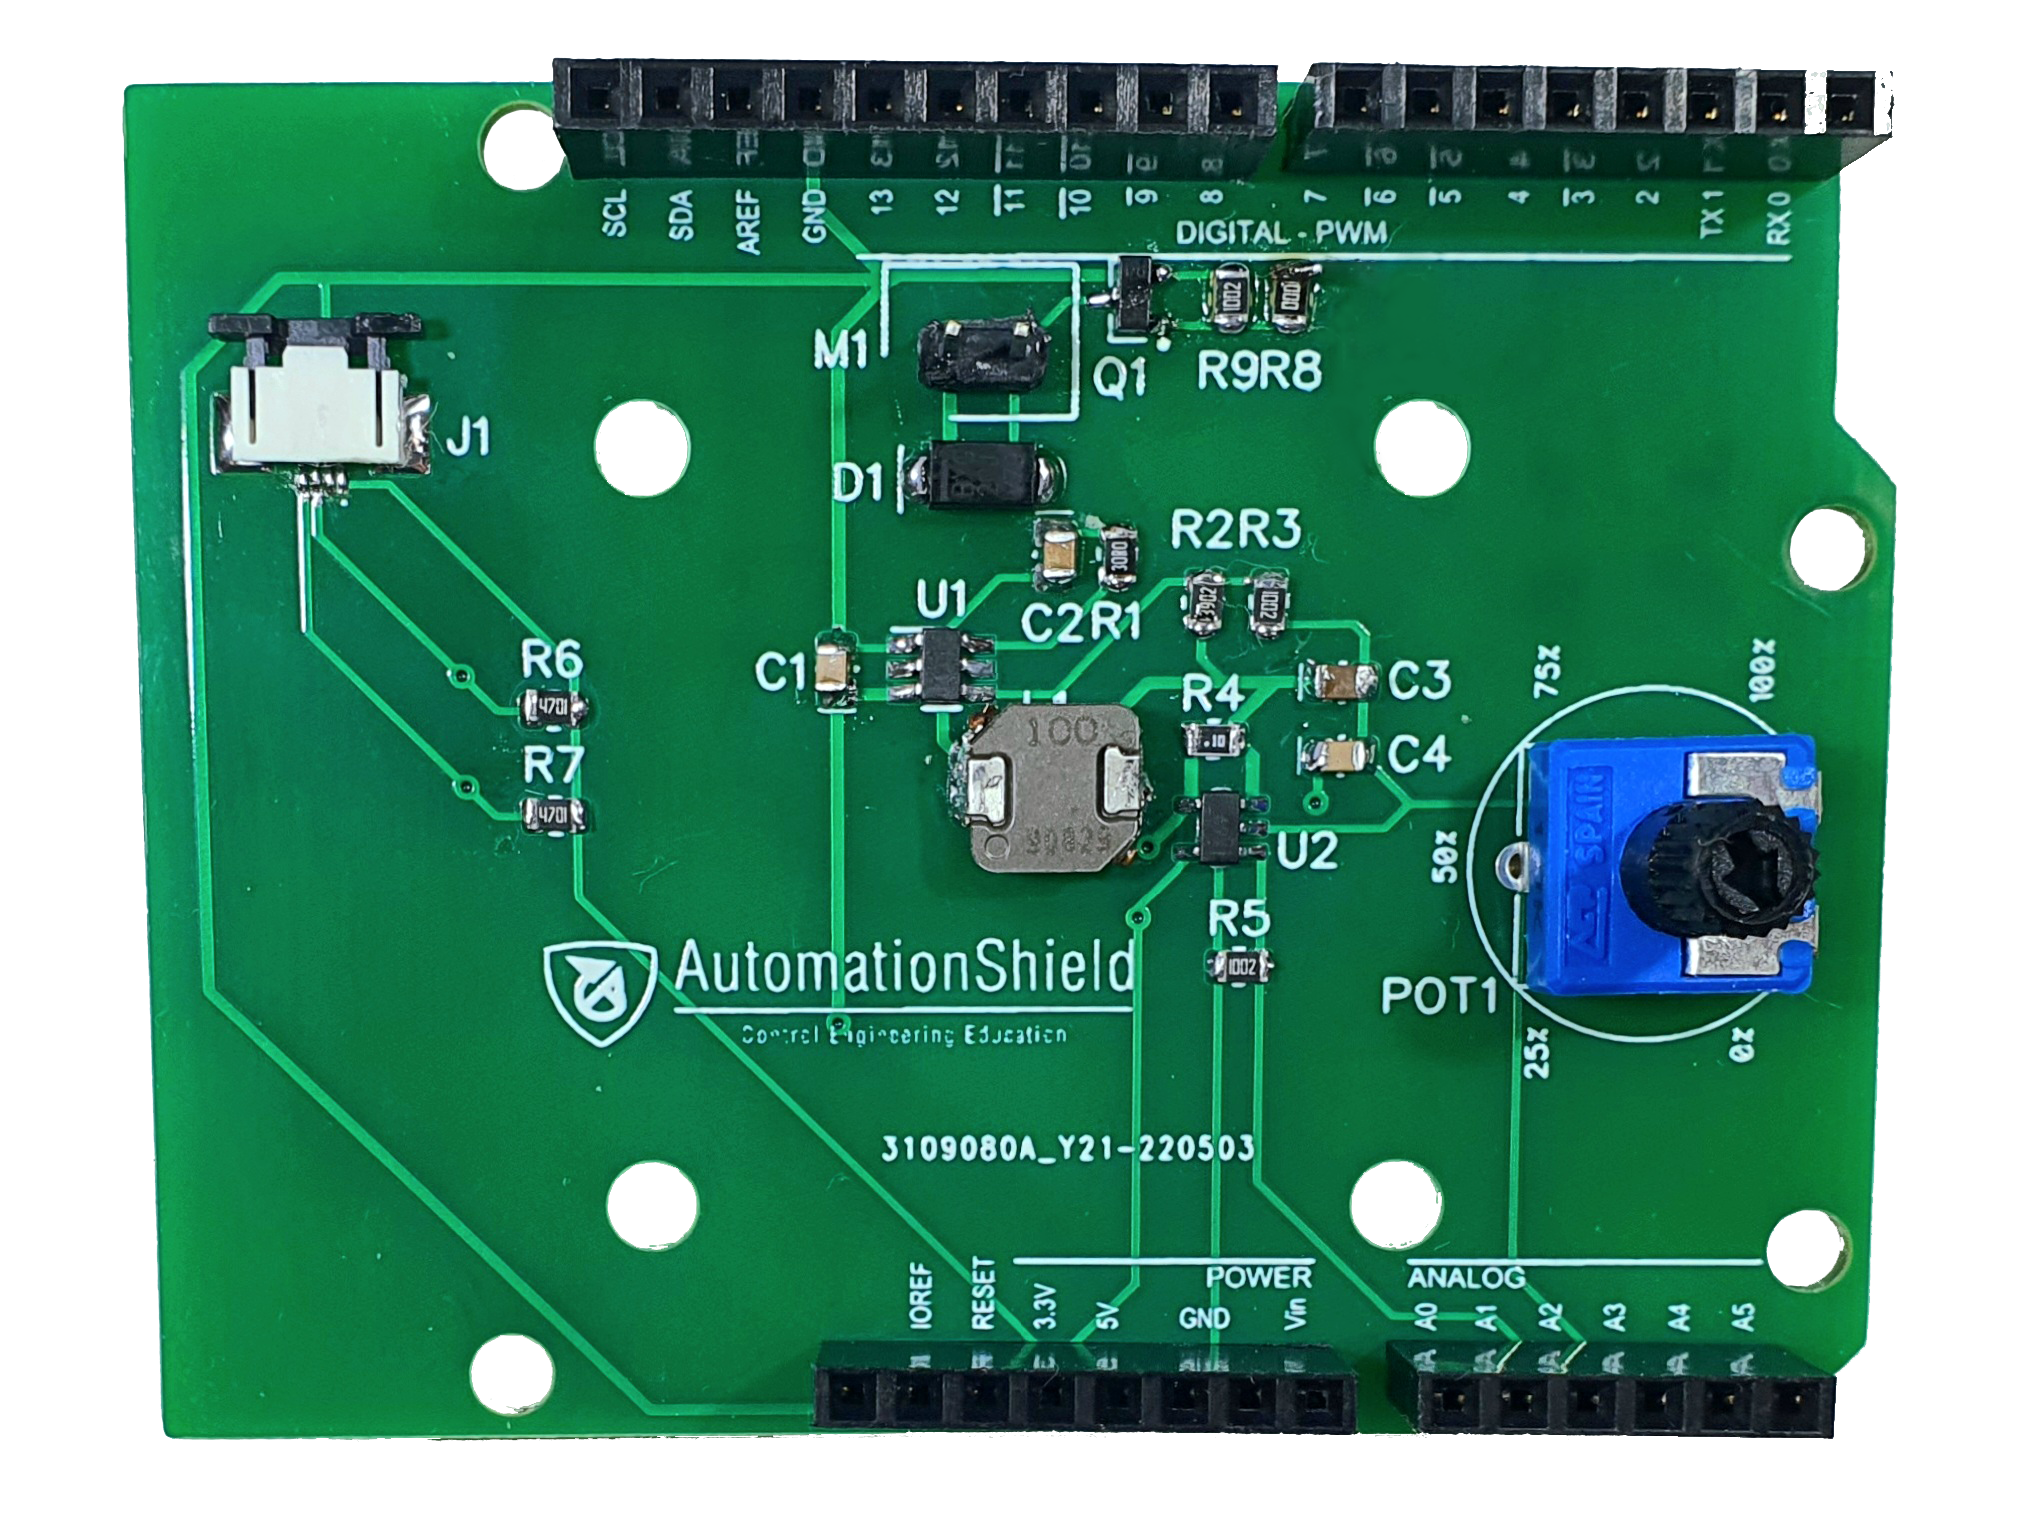
\includegraphics[width=110mm]{obr/NewAeroShield.png}
	\caption{Tretia verzia AeroShieldu.}\label{OBRAZOK 2.8}
\end{figure}

\begin{figure}[!tbh]
		\centering
	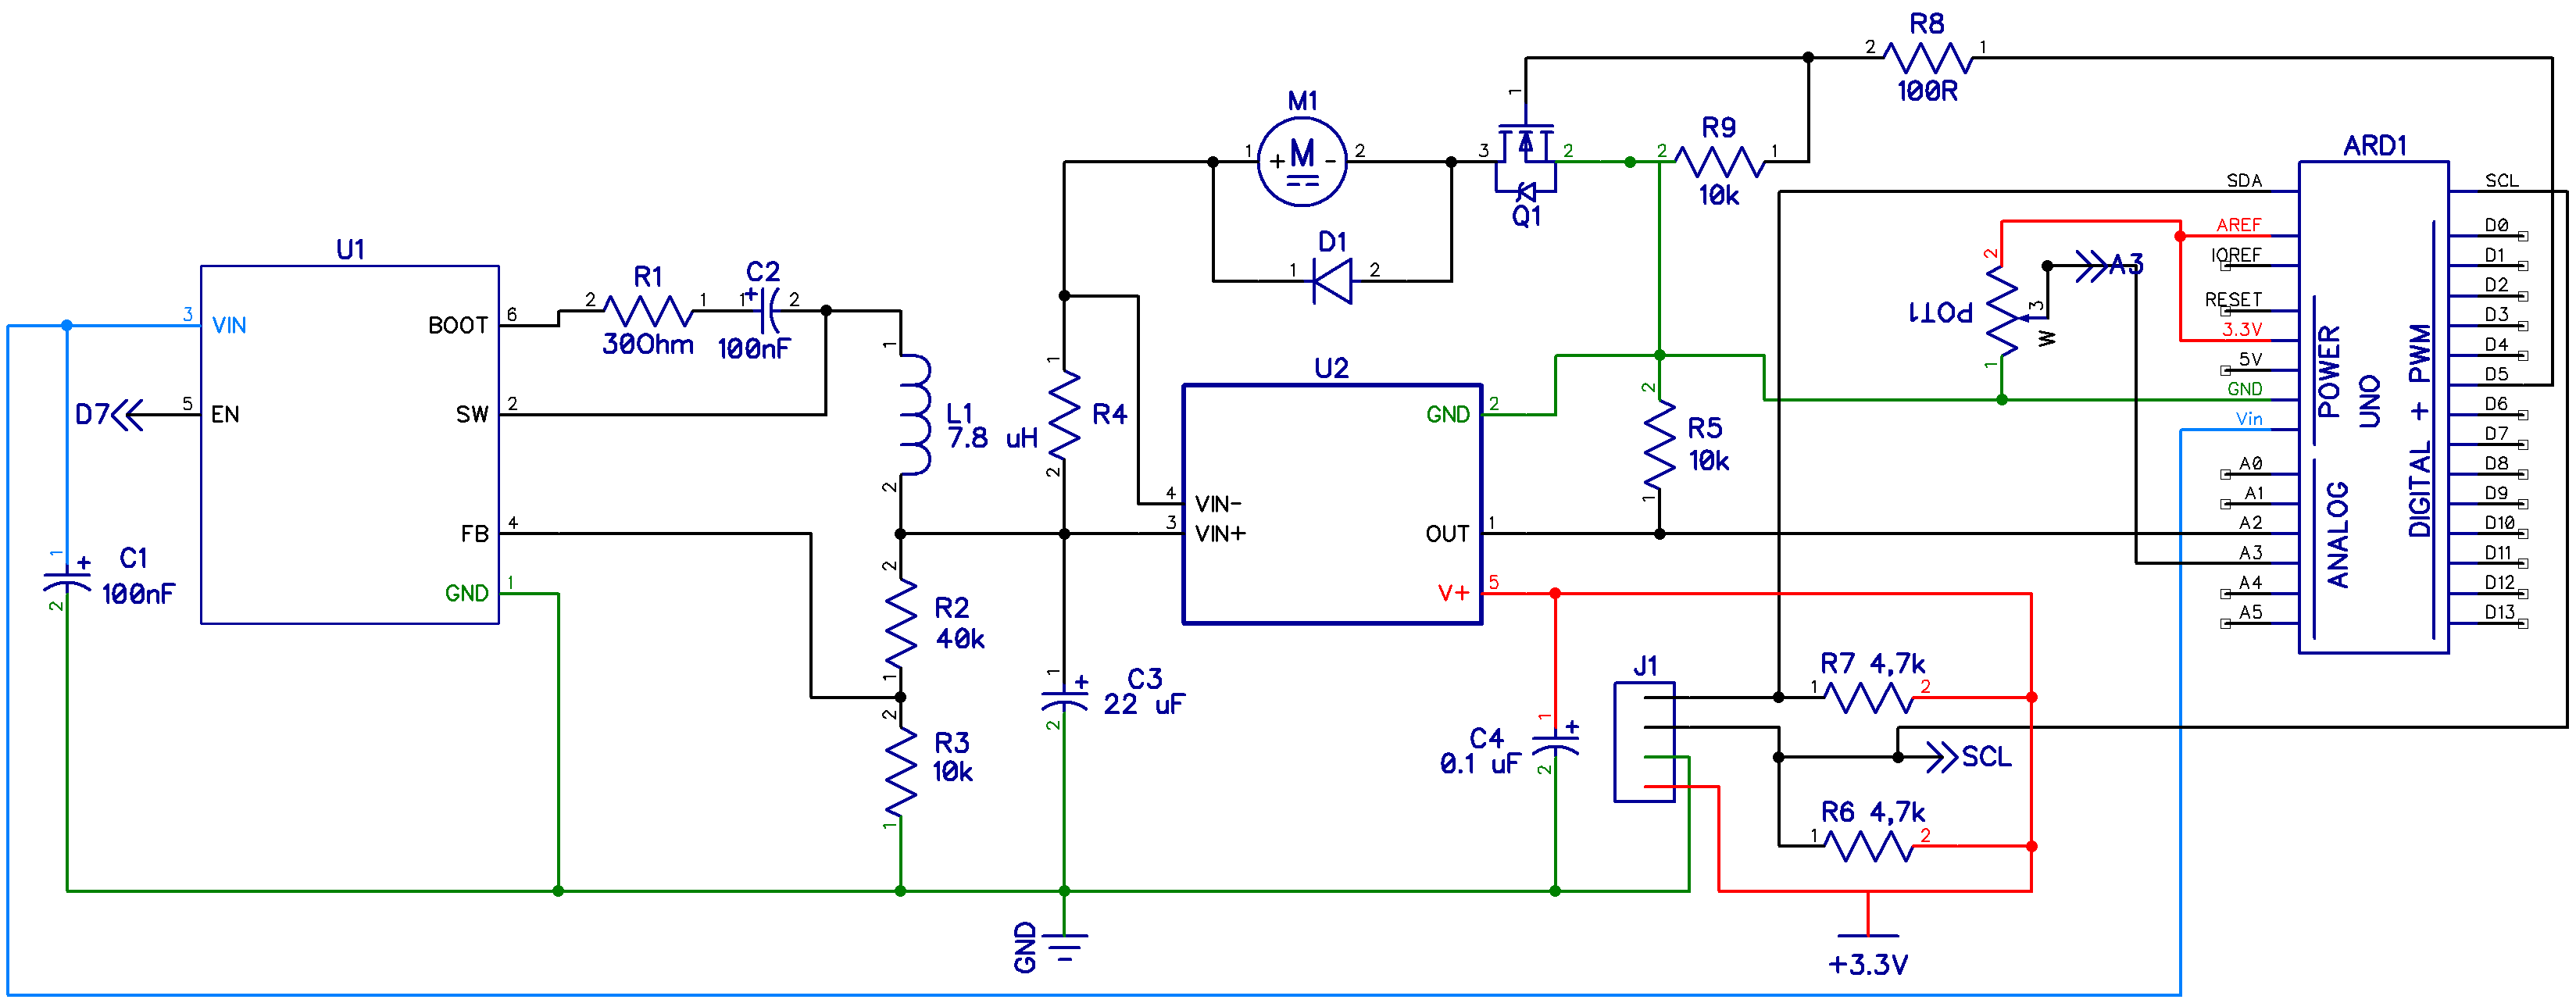
\includegraphics[width=\textwidth]{obr/TretiaSchema.png}
	\caption{Schéma zapojenia tretej verzie AeroShieldu.}\label{OBRAZOK 2.9}
\end{figure}
\section{Softvér}
\subsection{Arduino API}

Vývojové prostredie pre platformy arduino sa nazýva Arduino IDE\footnote[5]{Arduino Integrated Development Environment.} a využíva programovací jazyk C++ resp. jeho nadstavbu, s pridanými špecializovanými príkazmi a funkciami. C++ patrí medzi jeden z najviac používaných programovacích jazykov na svete. V rámci projektu AutomationShield existuje niekoľko rôznych shildov, ktoré však často využívajú rovnaké funkcie a príkazy. Z tohoto dôvodu bola vytvorená knižnica $"$AutomationShield$"$, ktorá v sebe zahŕňa niekoľko ďalších, často využívaných knižníc a súborov. Jedná sa napríklad o funkcie potrebné pri riadení pomocou PID regulátora, vzorkovanie programu alebo mapovanie premenných. O jednotlivých funkciách v rámci knižnice $"$AutomationShield$"$ si povieme viacej pri opise didaktických príkladov v časti:\ref{Didaktické príklady}.

V rámci programovania knižníc využívame objektovo orientované programovanie \newline (OOP)\cite{oop}. OOP je výhodné z hľadiska prehľadnosti, úpravy funkcií, redukcie nepotrebného alebo duplicitného kódu a mnoho ďalšieho. Pri OOP vytvárame dátové štruktúry nazývané objekty. Objekty majú svoje vlastnosti, metódy, udalosti a pomocou kombinácie týchto vlastností vykonávajú určité naprogramované činnosti. 

Knižnice väčšinou rozdeľujeme do dvoch súborov. Prvým z nich je \verb|header| teda hlavička s koncovkou .h a druhý \verb|source| alebo zdrojový dokument s koncovkou .cpp. Header slúži ako akýsi navádzač a sklad pre premenné a funkcie, ktorý následne komunikuje so source dokumentom v ktorom sú uložené samotné funkcie.
Takéto rozdelenie súborov má za ciel zrýchlenie kompilácie programu.


\subsubsection{Header}

Header súbor má niekoľko náležitostí ktoré obsahuje. Na začiatok deklarujeme súbor samotný. Robíme to pomocou príkazu \verb|#define|. Avšak ak by sa takáto deklarácia nachádzala vo viacerých súboroch, a teda header súbor by sa načítal niekoľko krát, spôsobovalo by to problém pri kompilácii kódu. Z toho dôvodu používame funkciu \verb|Include guard|, ktorá zamedzuje niekoľkonásobnému načítaniu rovnakých súborov. 

Hneď za definovaním knižnice AeroShild.h môžeme vkladať ďalšie knižnice, ktoré sú potrebné pre funkcie danej knižnice, a to pomocou príkazu \verb|#include|.

Za knižnicami následne určujeme premenné, ktoré môžu mať priradené fyzické čísla pinov na Arduine. Tieto premenné potom využívame buď na posielanie, alebo prijímanie signálov z daných pinov, ako aj na ukladanie rôznych konštánt. Príkaz \verb|#endif| vkladáme do záveru header súboru.

\begin{lstlisting}[caption={Ukážka zdrojového kódu headeru.},captionpos=b]
#ifndef AEROSHIELD_H	 	 // Pokial nie je definovana AEROSHIELD_H
#define AEROSHIELD_H	 	 // Definuj kniznicu AEROSHIELD_H

#include "AutomationShield.h"    // Hlavna kniznica AutomationShieldu
#include <Wire.h>                // Kniznica potrebna pre komunikaciu I2C
#include <Arduino.h>		 // Zakladna arduino kniznica

#define AERO_RPIN A3             // Vstup z potenciometra
#define VOLTAGE_SENSOR_PIN A2    // Vstup pre meranie prudu 
#define AERO_UPIN 5              // Aktuator

----------------------Zdrojovy kod----------------------

#endif			   	 // Koniec if podmienky 
\end{lstlisting}



V časti \verb|Zdrojovy kod|, vytvárame \verb|triedu| (class), ktorá v sebe zahŕňa funkcie a premenné, ktoré sa nazývajú \verb|objekty| (objects). Class obsahuje podmnožinu objektov, ktoré vieme prepájať a spájať vo väčšie celky, vďaka čomu vieme dosiahnuť veľmi komplexné funkcie. Týmto funkciám a premenným vieme obmedziť prístup resp. ich dosah v rámci programu, pomocou modifikátorov prístupu (access modifiers). Tieto modifikátory delíme do štyroch skupín. Základný modifikátor je \verb|default|, teda akýsi predvolený prístup, ktorý nadobúdajú všetky funkcie a premenné automaticky. Ďalšími modifikátormi sú \verb|public|, teda funkcie a premenné verejne prístupné v triede aj mimo nej a modifikátor \verb|privat|, ktorý obmedzuje prístup len pre danú triedu. Posledným modifikátorom prístupu je \verb|protected|, čo je prístup chránený. V header súbore sa môže nachádzať jedna, alebo viacero tried, záleží to od logicky deliteľných úsekov kódu, alebo od preferencie programátora. 

Rozdelenie na public a privat má zmysel hlavne v prípade ak chceme mať zadefinované premenné, pri ktorých nechceme aby sa dala externe zmeniť ich hodnota alebo typ. V prípade privat, takáto zmena nie je možná. Zmeniť takúto premennú môžeme len jej ručným prepísaním v zdrojovom súbore. V časti private deklarujeme funkcie, ktoré následne využívame v rámci triedy, alebo slúžia ako pomocné funkcie pri tvorbe komplexnejších častí kódu. V časti public sú funkcie viditeľné a schopné interagovať s inými triedami, ako aj s inými knižnicami. 


\subsubsection{Source}

Keďže všetky potrebné knižnice sa už definovali a načítavali v súbore header, stačí nám už len časti source a header prepojiť. Urobíme tak pomocou príkazu \code{#include "AeroShield.h"}, ktorý vložíme na začiatok súboru. Ďalej v súbore deklarujeme jednotlivé funkcie, ktoré majú na začiatku zápisu, zvolený istý dátový typ. Dátové typy funkcií poznáme rôzne. Vyberáme si ich na základe potreby ako chceme aby funkcia reagovala resp. aké hodnoty by mala prenášať. Dátové typy\footnote[6]{všetky hodnoty sú platné pre arduino UNO, pre iné typy arduina sa hodnoty môžu líšiť} poznáme nasledovné\cite{datovetypy}: 

\begin{table}[!ht]
	\centering
	\begin{tabular}{|p{0.22\textwidth} | p{0.22\textwidth} |p{0.22\textwidth} |p{0.22\textwidth} |}
		\hline
		\thead{dátový typ} & \thead{vlastnosti} & \thead{dátový typ} & \thead{vlastnosti} \\ \hline
		\textbf{array} & skupina premenných s priradeným indexom. Maximálna veľkosť je obmedzená veľkosťou pamäte RAM & \textbf{short }& 16 bitové celé čísla \\ \hline
		\textbf{boolean} & má buď hodnotu 0-nepravda, alebo 1-pravda & \textbf{char array }& spojenie viacerých dát typu char ukončené hodnotou null \\\hline
		\textbf{byte} & 8 bitové čísla od 0 do 255 & \textbf{string-object} & podobná funkcia ako object v header súbore \\ \hline
		\textbf{double} & rovnaké ako float & \textbf{unsigned char} & 8-bit znaky od 0 do 255 \\ \hline
		\textbf{float} & 32 bitové desatinne čísla $\pm$3.4028235E$+38$ & \textbf{unsigned int }& 16 bitové kladné celé čísla od 0 do 2$^{16}$-1 \\\hline
		\textbf{char} & 8 bit ascii tabulka & \textbf{unsigned long} & 32 bitové kladné celé čísla od 0 do 2$^{32}$-1 \\\hline
		\textbf{int} & 16 bitové celé čísla & \textbf{void }& nevracia naspäť žiadne informácie \\ \hline
		\textbf{long }& 32 bitové celé čísla & \textbf{word} & 16-bit číslo bez znamienka \\ \hline
    \end{tabular}
\caption{Dátové typy}
\label{tabulka typov}
\end{table}

\subsubsection{Popis použitých funkcií z knižnice AutomationShield}

Pri rôznych veľkostiach a rozsahoch číselných stupníc, je dobré vyjadrovať hodnoty v percentách, namiesto ich absolútnej hodnoty. Arduino ponúka funkciu \verb|map()|, ktorá však pracuje len s dátovým typom integer. Aby sme docielili vyššiu presnosť, potrebujeme mapovať dátový typ float. Na tento účel nám slúži funkcia mapFloat do ktorej vstupuje veličina x, ktorej priradíme požadované hodnoty. Funkcie funguje na základe princípu lineárneho mapovania\cite{linearMap}.  

\begin{lstlisting}[caption={Zdrojový kód funkcie mapFloat.},captionpos=b]
float AutomationShieldClass::mapFloat(float x, float in_min, float in_max, float out_min, float out_max) 
{
return (x - in_min) * (out_max - out_min) / (in_max - in_min) + out_min; 
}
\end{lstlisting}

Ďalšou z funkcií použitých z knižnice AutomationShield je serialPrint. Funkcia vypisuje zvolený text na sériový monitor arduina. 

\begin{lstlisting}[caption={Zdrojový kód funkcie serialPrint.},captionpos=b]
 void AutomationShieldClass::serialPrint(const char *str){   
	#if ECHO_TO_SERIAL           // Pokial je tato funkcia povolena                       
	Serial.print(str);           // Vypis na seriovy monitor                       
	#endif 		// Koniec
}
\end{lstlisting}

\subsubsection{Popis použitých funkcií z knižnice AeroShield}


Keďže na AeroShielde využívame senzor hall efektu, musíme s ním v prvom rade nadviazať komunikáciu pomocou sériovej komunikácie I$^{2}$C.

Táto komunikácia funguje na princípe master-slave, kedy master je nadriadený a slave je podriadené zariadenie, s ktorým master komunikuje. Master môže naraz komunikovať s viacerými zariadeniami a to na základe jedinečných adries zariadení, ktoré sa medzi sebou striedajú v komunikácii.

 Protokol I$^{2}$C využíva na odosielanie a prijímanie údajov dva vodiče resp. dve linky: 
\begin{itemize}
\item sériovú dátovú linku (SDA-serial data), cez ktorú sa posielajú údaje, 
\item sériovú hodinovú linku (SCL-serial clock), na ktorú arduino v pravidelných intervaloch posiela impulzy. 
\end{itemize}

Hodinový pin udáva tempo komunikácie a je ovládaný mastrom. Mení stav v pravidelných impulzoch z 0 (low), na 1 (high). Pri každej takejto zmene je na dátový pin poslaný jeden bit informácie. Tieto bity najskôr obsahujú adresu zariadenia slave s ktorým chce master komunikovať, následne sa odosielajú bity príkazov. Keď sa táto informácia celá odošle, slave vykoná požiadavku a ak je to vyžadované, môže spätne mastrovi poslať údaje. Všetky tieto bity informácií sa posielajú na linke SDA\cite{idvac}.

   

\subsubsection{Funkcia readOneByte()}

 Funkcia \code{int AeroShield::readOneByte()}, získava 1 bajt informácii zo senzoru. Túto funkciu využívame napríklad na čítanie polohy kyvadla. 

\begin{lstlisting}[caption={Zdrojový kód funkcie readOneByte.},captionpos=b]
int AeroShield::readOneByte(int in_adr)         
{
	int retVal = -1;	 // Zadefinovanie pomocnej premennej
	Wire.beginTransmission(_ams5600_Address);// Zaciatok komunikacie 
	Wire.write(in_adr);	// Poziadavka na zaznamenianie uhlu kyvadla 
	Wire.endTransmission();	// Koniec komunikacie zo strany mastra
	Wire.requestFrom(_ams5600_Address, 1);	// Ziadost na odpoved  
	while (Wire.available() == 0);	// Cakaj pokial odpoved nepride  
	
	retVal = Wire.read();	// Zaznamenanie odpovede 
	
	return retVal;	// Zaslanie odpovede 
}
\end{lstlisting}

Ako môžeme vidieť v kóde funkcie, master najskôr osloví zariadenie slave, pomocou jeho adresy. Pri senzore \verb|AS5600| je adresa zariadenia v hexadecimálnej podobe 0x36. Následne zašle od výrobcu predprogramovanú žiadosť, ktorá zaznamená aktuálnu polohu magnetu resp. kyvadla. Následne je zaslaná požiadavka na odpoveď zo strany slave zariadenia, ktorá je zaznamenaná a odoslaná späť na miesto, z ktorého bola funkcia privolaná.

\subsubsection{Funkcia readTwoBytes()}

Funkcia \code{word AeroShield::readTwoBytes()} je podobná predošlej funkcii, s tým rozdielom, že získané su dva bajty informácií. Na konci funkcie ešte prebieha bitový posun\footnote[6]{Bitový posun je operácia vykonávaná so všetkými bitmi binárnej hodnoty, pri ktorej sa posúvajú o určený počet miest doľava alebo doprava\cite{biteShift}.}. 

\begin{lstlisting}[caption={Zdrojový kód funkcie readTwoBytes.},captionpos=b]
word AeroShield::readTwoBytes(int in_adr_hi, int in_adr_lo)        
{
	word retVal = -1;		// Zadefinovanie pomocnej premennej
	/* citanie "Low" bajtu */
	Wire.beginTransmission(_ams5600_Address);// Zaciatok komunikacie 
	Wire.write(in_adr);	// Poziadavka na zaznamenianie uhlu kyvadla 
	Wire.endTransmission();	// Koniec komunikacie zo strany mastra
	Wire.requestFrom(_ams5600_Address, 1);	// Ziadost na odpoved  
	while (Wire.available() == 0);	// Cakaj pokial odpoved nepride  

	int low = Wire.read();     	// Ulozenie prveho bajtu 
	/* citanie "High" bajtu */
	Wire.beginTransmission(_ams5600_Address);// Zaciatok komunikacie 
	Wire.write(in_adr);	// Poziadavka na zaznamenianie uhlu kyvadla 
	Wire.endTransmission();	// Koniec komunikacie zo strany mastra
	Wire.requestFrom(_ams5600_Address, 1);	// Ziadost na odpoved  
	while (Wire.available() == 0);	// Cakaj pokial odpoved nepride  
	
	word high = Wire.read();   	// Ulozenie druheho bajtu 
	
	high = high << 8;          	// Posun bitov
	retVal = high | low;
	
	return retVal;	   	  	// Zaslanie odpovede 
}
\end{lstlisting}

\subsubsection{Funkcia detectMagnet()}

Ďalšou dôležitou funkciou, je zistiť prítomnosť magnetu na kyvadle. Túto úlohu vykonáva funkcia \code{int AeroShield::detectMagnet()}. Využívame ju vždy pri inicializácii AeroShieldu, na to aby sme zistili či nenastali problémy s magnetom, alebo so senzorom samotným. Funkcia komunikuje so senzorom, a na základe výstupu vieme určiť či bol magnet detegovaný. Funkcia nám vráti na výstupe 1- pokiaľ sa magnet nachádza pri senzore a 0- pokiaľ magnet nie je prítomný, alebo je príliš vzdialený od senzoru. 

\begin{lstlisting}[caption={Zdrojový kód funkcie detectMagnet.},captionpos=b]
int AeroShield::detectMagnet() 
{
	int magStatus;		// Pomocna premenna  
	int retVal = 0;		// Pomocna premenna
	magStatus = readOneByte(_stat);	// Prebieha komunikacia so senzorom                        
	
	if (magStatus & 0x20)		// Pokial je podmeinka splnena vrat 1, pokial nie je splnena vrat 0 
	retVal = 1;
	
	return retVal;			// Zaslanie odpovede 
}
\end{lstlisting}

\subsubsection{Funkcia getMagnetStrength()}

Pre správnosť fungovania hall senzoru je dôležité dodržať správnu vzdialenosť magnetu od senzoru. Výrobca udáva že najideálnejšia vzdialenosť je 0.5-3mm, v závislosti na sile a veľkosti magnetu. Bolo by nepraktické túto vzdialenosť merať ručne, použijeme preto funkciu \code{int AeroShield::getMagnetStrength()}. Môžeme si všimnúť že táto funkcia používa rovnaký príkaz na komunikáciu so senzorom, ako aj funkcia \code{detectMagnet()} a to síce \verb|_stat|. Z toho vyplýva že \code{detectMagnet()} kontroluje nielen prítomnosť magnetu, ale aj jeho správnu vzdialenosť. Pokiaľ teda dostaneme z funkcie \code{detectMagnet()} ako výsledok 1, vieme že magnet je prítomný a zároveň v ideálnej vzdialenosti. Funkcia \code{getMagnetStrength()} je teda iba doplňujúcou funkciou, ktorá nám určí či sa magnet nachádza príliš blízko, alebo naopak veľmi ďaleko od senzoru. 

\begin{lstlisting}[caption={Zdrojový kód funkcie getMagnetStrength.},captionpos=b]
int AeroShield::getMagnetStrength()   
{
	int magStatus;                  // Pomocna premenna 
	int retVal = 0;                 // Pomocna premenna
	magStatus = readOneByte(_stat);	// Prebieha komunikacia so senzorom       
	
	if (detectMagnet() == 1)	// Pokial je splnena podmienka detectMagnet()
	{
		retVal = 2;  // Vrat 2, magnet je v idelnej vzdialenosti
		if (magStatus & 0x10)
		retVal = 1;  // Vrat 1, magnet je v prilis daleko
		else if (magStatus & 0x08)
		retVal = 3;  // Vrat 3, magnet je v prilis blizko
	}
	
	return retVal;                  // Zaslanie odpovede  
}
\end{lstlisting}

\subsubsection{Funkcia getRawAngle()}

Táto funkcia slúži na čítanie uhlu kyvadla. Výstupom tejto funkcie, je číslo s rozsahom 12bitov, teda číslo od 0 do 4096, ktoré udáva momentálnu polohu kyvadla. 

\begin{lstlisting}[caption={Zdrojový kód funkcie getRawAngle.},captionpos=b]
word AeroShield::getRawAngle() 
{
	return readTwoBytes(_raw_ang_hi, _raw_ang_lo); // Prebieha komunikacia so senzorom, ktory rovno vrati vysledok pomocou prikazu return 
}
\end{lstlisting}

\subsubsection{Funkcia begin()}

Prvou z funkcií mimo komunikácie s hall senzorom je \code{float AeroShield::begin(bool isDetected)}, do ktorej vstupuje výsledok z funkcie \code{detectMagnet()} ako premenná \verb|isDetected|. Funkcia \code{begin()} nastaví pin potrebný na ovládanie akčného člena, pomocou príkazu \verb|pinMode|, ako výstup (OUTPUT). Zároveň inicializuje sériovú komunikáciu I$^{2}$C. Príkaz na započatie komunikácie I$^{2}$C sa pri rôznych typoch dosiek, resp. architektúr mikroradiča Arduino líši. Použijeme preto podmienku \verb|#ifdef| za ktorou nasleduje typ architektúry daného mikroradiča a príslušný príkaz pre začiatok sériovej komunikácie I$^{2}$C. V prípade Arduino UNO, je to príkaz \verb|Wire.begin()|. 

Zároveň je vo funkcii \code{begin()}, pomocou if podmienky, kontrolovaná premenná \verb|isDetected|. Pokiaľ bol magnet detegovaný, vypíše na sériový port správu "Magnet detected$"$ a while\footnote[8]{Cyklus while sa bude opakovať nepretržite, pokiaľ sa výraz vnútri zátvoriek () nestane nepravdivým.} cyklus, sa pomocou príkazu \verb|break| ukončí. Pokiaľ magnet detegovaný nebol, vypíše "Can not detect magnet", no while cyklus pokračuje.  


\begin{lstlisting}[caption={Zdrojový kód funkcie begin.},captionpos=b]
float AeroClass::begin(void){                       
	bool isDetected = AeroShield.detectMagnet(); 
	// Detekcia magnetu 
	pinMode(AERO_UPIN,OUTPUT);	// Pin aktuatora
	
	#ifdef ARDUINO_ARCH_AVR		// Pre dosky s architekturov AVR
	Wire.begin();			// Pouzi objekt Wire
	#elif ARDUINO_ARCH_SAM      	// Pre dosky s architekturov SAM
	Wire1.begin();			// Pouzi objekt Wire1
	#elif ARDUINO_ARCH_SAMD     	// Pre dosky s architekturov SAMD
	Wire.begin();			// Pouzi objekt Wire
	#endif
	
	if(isDetected == 0 ){       	// Pokial magnet nie je detegovany
		while(1){               // While podmienka
		 if(isDetected == 1 ){	// Pokial sa magnet deteguje
		  AutomationShield.serialPrint("Magnet detected \n");	
		break;		    // Koniec while podmienky
		}
		else{               // Pokial magnet nie je detegovany
		  AutomationShield.serialPrint("Can not detect magnet \n");
			}
		}
	}       
} 
\end{lstlisting}

\subsubsection{Funkcia calibration()}

Funkcia \code{calibration()} slúži na prepočet a zaznamenanie nulovej polohy kyvadla, teda takej kedy výkon motora=0\%. V ideálnom prípade by sa kyvadlo vždy po vypnutí motora vrátilo do rovnakej východzej polohy. Avšak kyvadlo je prepojené s motorom a shieldom pomocou káblov, ktoré tvoria odpor a teda kyvadlo sa vždy zastaví v inej nulovej polohe. 

Do funkcie vstupuje hodnota aktuálneho uhlu kyvadla, z funkcie \code{getRawAngle()} ako premenná \verb|RawAngle|. Funkcia na začiatok vypíše text "Calibration running...$"$ a motorček zapneme na štvrť sekundy na výkon 20\%. Kyvadlo sa začne kývať a počkáme štyri sekundy, pokiaľ sa ustáli. Keď je kyvadlo ustálené zaznamenáme jeho hodnotu do premennej \verb|startangle|. Následne prebieha for cyklus ktorý zvukovo informuje o dokončenej kalibrácii pomocou troch pípnutí. 

\begin{lstlisting}[caption={Zdrojový kód funkcie calibration.},captionpos=b]
float AeroShield::calibration(word RawAngle) {  
	AutomationShield.serialPrint("Calibration running...\n");  
	startangle=0;              // Vynulovanie premennej 
	analogWrite(AERO_UPIN,50); // Spustenie motora na vykon 20%
	delay(250);                // Cakaj 0.25s 
	analogWrite(AERO_UPIN,0);  // Vypnutie motora
	delay(4000);               // Cakaj 4s
	
	startangle = RawAngle;     // Uloz hodnotu nuloveho uhla
	analogWrite(AERO_UPIN,0);  // Poistne vypnutie motora 
	for(int i=0;i<3;i++){      // Funkcia na zvukovu signalizaciu
		analogWrite(AERO_UPIN,1);     // Zapnutie motora
		delay(200);                   // Cakaj
		analogWrite(AERO_UPIN,0);     // Vypnutie motora
		delay(200);                   // Cakaj
	}
	
	AutomationShield.serialPrint("Calibration done");
	return startangle;                    // Vrat hodnotu 
}
\end{lstlisting}

\subsubsection{Funkcia convertRawAngleToDegrees()}

Ako sme už spomínali v sekcii \ref{meruhl}, zaznamenávaná hodnota uhlu kyvadla je v rozmedzí od 0 do 4096 a tieto hodnoty sú priamo úmerné zo stupňami od 0\textdegree  do 360\textdegree. 1\textdegree   predstavuje hodnotu približne 11.77 vo formáte raw. Funkcia teda prenásobí raw hodnotu číslom  $\dfrac{360\textdegree}{4096}$ =0.087\textdegree. Výsledkom rovnice je prepočítaný uhol v stupňoch. 

\begin{lstlisting}[caption={Zdrojový kód funkcie convertRawAngleToDegrees.},captionpos=b]
float AeroShield::convertRawAngleToDegrees(word newAngle) {  
	float ang = newAngle * 0.087;    // 360/4096=0.087 x rawHodnota                             
	return ang;                      // Vrat hodnotu
}
\end{lstlisting}


\subsubsection{Funkcia referenceRead()}

Funkcia \code{referenceRead()} slúži na čítanie hodnoty z potenciometra, ktorý sa nachádza na shielde, a jeho následne premapovanie do percentuálnej podoby. Potenciometer využívame na manuálne ovládanie AeroShieldu a v ďalších funkciách, sa využíva hlavne jeho percentuálna hodnota. Vrátená hodnota je typu float, v škále od 0.0\% do 100.0\%. 

\begin{lstlisting}[caption={Zdrojový kód funkcie referenceRead.},captionpos=b]
	  float AeroShield::referenceRead(void) {      
		referencePercent = AutomationShield.mapFloat(analogRead(AERO_RPIN), 0.0, 1024.0, 0.0, 100.0);  
		 // Premapovanie originalnej hodnoty 0.0-1023 na percentualny rozsah 0.0-100.0
		return referencePercent;      // Vrat percentualnu hodnotu 
	}
\end{lstlisting}
	
\subsubsection{Funkcia actuatorWrite()}	
	
Na ovládanie motora resp. jeho otáčok, používame funkciu \code{actuatorWrite()}. Do funkcie vstupuje percentuálna hodnota výkonu motora. Táto hodnota je premapovaná na PWM signál, ktorý využívame na ovládanie motora. Tento signál následne vstupuje do ochrannej funkcie \code{constrainFloat()}, ktorá zabezpečí aby sa hodnota PWM signálu mohla pohybovať len v rozmedzí od 0.0 do 255.0. 
	
	
\begin{lstlisting}[caption={Zdrojový kód funkcie actuatorWrite.},captionpos=b]
	void AeroShield::actuatorWrite(float PotPercent) {   
		float mappedValue = AutomationShield.mapFloat(PotPercent, 0.0, 100.0, 0.0, 255.0);       
		// Vstupna percentualna hodnota 0.0-100.0 premapovana na hodnoty 0.0-255.0
		mappedValue = AutomationShield.constrainFloat(mappedValue, 0.0, 255.0);  
		// Bezpecnostna funkcia obmedzenia premapovanej hodnoty
		analogWrite(AERO_UPIN, (int)mappedValue);  // Zapisanie hodnoty na pin
	}
\end{lstlisting}
	
	
\subsubsection{Funkcia currentMeasure()}	
	
Poslednou funkciou AeroShieldu je \code{currentMeasure()}. Funkcia slúži na zaznamenávanie prúdu, ktorý odoberá motor kyvadla. Fungovanie snímača je opísané v sekcii \ref{merprud}. Funkcia slúži na prepočítanie zaznamenanej hodnoty napätia na prúd. Pre presnejšie výsledky merania, využívame priemernú hodnotu prúdu, ktorú získavame pomocou for cyklu. 

Nepresnosť vzniká v dôsledku ovládania motora PWM signálom. Tým že je motor prerušovane vypínaný a zapínaný, kolísa aj veľkosť odoberaného prúdu. 

Výsledná hodnota prúdu prechádza úpravami, pomocou dvoch korekčných premenných, ktoré sme získali vďaka meraniam prúdu pomocou multimetra, a následným porovnaním týchto hodnôt oproti hodnotám zo senzora. 

Prevod z napätia na prúd robíme podľa pokynov uvedených v zdrojovom dokumente senzoru. Pri tomto prevode využívame hodnotu shunt rezistora \verb|RS|, ako aj hodnotu rezistora \verb|RL|. 
  
	
\begin{lstlisting}[caption={Zdrojový kód funkcie currentMeasure.},captionpos=b]	
float AeroShield::currentMeasure(void){  
	for(int i=0 ; i<repeatTimes ; i++){     // For cyklus
	voltageValue= analogRead(VOLTAGE_SENSOR_PIN);     
	// Citanie hodnoty zo senzoru INA169 
	voltageValue= (voltageValue * voltageReference) / 1024;    
	// Mapovanie hodnoty zo senzoru, na realnu hodnotu napatia(referencne napatie je 5V)
	current= current + correction1-(voltageValue / (10 * ShuntRes));    
                // Vzorec na vypocet prudu
                // Is = (Vout x 1k) / (RS x RL)
}                                                                         	
	float currentMean= current/repeatTimes;   
	// Vypocet priemernej hodnoty  
	currentMean= currentMean-correction2;       // Korekcia
	if(currentMean < 0.000) currentMean= 0.0;                 
	                    // Korekcia nulovej hodnoty
	current= 0;         // Vynulovanie pomocnych premennych   
	voltageValue= 0;    // Vynulovanie pomocnych premennych   
	return currentMean; // Vrat hodnotu prudu v amperoch
}
\end{lstlisting}
	
\subsection{MATLAB}	
\label{matlabik}
	
V tomto programe, rovnako ako pri Arduino IDE, vieme príkazy a funkcie zapisovať do knižnice, odkiaľ si potom jednotlivé položky voláme do hlavného kódu. Z toho dôvodu bola zostavená knižnica \verb|AeroShield.m|. Knižnice v MATLABE môžu mať podobu súborov \verb|Header| a \verb|Source|, alebo funkcie zapíšeme len do jedného súboru s koncovkou \verb|.m|. 

V našom prípade sa jedná o jeden súbor na ktorého začiatku definujeme triedu súboru, pomocou príkazu \code{classdef AeroShield < handle ... end}. Za príkazom \verb|classdef| nasleduje názov našej triedy \verb|AeroShield| a porovnávací symbol $<$, za ktorým nasleduje $"$super trieda$"$ \verb|handle|. Super, alebo nad-trieda \verb|handle| je abstraktná trieda, ktorej inštancia sa nedá vytvoriť priamo. Táto trieda sa využíva na odvodenie iných tried, ktoré sú už konkrétnymi triedami, ktorých inštancie sú objektmi handle. 

Každá trieda môže následne obsahovať jeden alebo viacero triednych blokov: 
\begin{itemize}
	\item Properties(atribúty) ...end- Vymedzuje blok kódu, ktorý definuje vlastnosti s rovnakými nastaveniami atribútov.
	\item Methods(atribúty)    ...end- Má rovnaký názov ako trieda v ktorej sa nachádza a vracia inicializovaný objekt triedy.
	\item Events(atribúty)     ...end- Vymedzuje blok kódu, v ktorom nastane istá preddefinovaná udalosť, napr. zmena stavu. 
	\item Enumeration(atribúty)...end- Vytvorí zoznam hodnôt/premenných. 
\end{itemize}

V AeroShield knižnici máme definované dva triedne bloky typu properties. V prom bloku sa nachádzajú objekty pre dosku arduino a hall senzor. V druhom bloku definujeme všetky premenné ktoré budeme ďalej v kóde využívať. Jedná sa hlavne o názvy a čísla pinov, ktoré používame na čítanie alebo zapisovanie hodnôt, ako aj o premenné, na výpočet prúdu odoberaného motorom. 

\begin{lstlisting}[caption={Knižnica AeroShield.m properties.},captionpos=b]
classdef AeroShield < handle

properties
	arduino;		% objekt dosky arduino 
	as5600;			% objekt hall senzoru
end

properties(Constant)
	AERO_UPIN = 'D5';          % pin aktuatora 
	AERO_RPIN = 'A3';          % pin potenciometra
	VOLTAGE_SENSOR_PIN = 'A2'; % pin na meranie prudu
	
	voltageReference = 5.0;    % referencne hodnota napatia 
	ShuntRes = 0.1;            % hodnota shunt rezitora v ohmoch
	correction1 = 4.1220;	   % korekcia  				  
	correction2 = 0.33;        % korekcia
	repeatTimes = 50;          % pocet cyklov pre vypocet priemernej hodnoty prudu 
end		
\end{lstlisting}
		
Nasleduje triedy blok \verb|methods|, v ktorom sú všetky funkcie, ktoré budeme volať do hlavnej časti kódu. Keďže logika funkcií je rovnaká ako pri súbore \verb|Source|, nebudeme si funkcie vysvetľovať po jednom. Dôležité je poznamenať, že pokiaľ nám do funkcie nejaká premenná vstupuje, zapisujeme ju v zátvorke za príkazom funkcie \code{function nazovFunkcie(AeroShieldObject, vstupnaPremenna)}. Naopak, pokiaľ z funkcie nejaká premenná vychádza, túto premennú deklarujeme pred názvom funkcie \code{function vystupnaPremenna = nazovFunkcie(AeroShieldObject)}. Pre pochopenie si ešte ukážeme časť kódu \code{function begin(AeroShieldObject)}, v ktorej prebieha tvorba objektov pre arduino a hall senzor. Proces odvolávania sa na objekt \verb|arduino|, funguje cez názov triedy \verb|AeroShield|, v ktorom sa odvolávame na \verb|Object|. Príkaz \verb|arduino()| slúži na vyhľadanie dosky arduino, pripojenej do počítača a nastavenie parametrov potrebných na komunikáciu. Rovnako sa odvolávame aj na objekt \verb|as5600|, ktorý vytvoríme pomocou príkazu \verb|device()|, v ktorom zadávame objekt dosky arduino, a adresu zariadenia I$^2$C. Poslednou funkciou je vypísanie správy a konfiguráciu pinu \verb|AERO_UPIN| ako výstup. 

\begin{lstlisting}[caption={Knižnica AeroShield.m properties.},captionpos=b]
function begin(AeroShieldObject)          % funkcia inicializacie
	AeroShieldObject.arduino = arduino(); % tvorba arduino objektu
	AeroShieldObject.as5600 = device(AeroShieldObject.arduino,'I2CAddress',0x36); % tvorba objektu sonzoru
	configurePin(AeroShieldObject.arduino,AeroShieldObject.AERO_UPIN, 'DigitalOutput') % konfiguracia pinu ako vystup
	disp('AeroShield initialized.') % vypis spravu
end
\end{lstlisting}

Zostávajúce funkcie, ako aj celý zdrojový kód knižnice \verb|AeroShield.m| sa nachádza v prílohe na strane \pageref{AeroShield.m}. 

\newpage
\subsection{Simulink}

Simulink, narozdiel od MATLABU alebo Arduino IDE, využíva grafické programátorské prostredie, ktoré je založené na prepájaní funkčných blokov, vyberaných z knižnice. Pre prácu s Arduinom, v rámci Simulinku, existuje knižnica \textit{Simulink Support Package for Arduino Hardware}, ako aj knižnica AeroLibrary obr.\ref{OBRAZOK 2.6.4}, ktorú využívame priamo pre funkcie AeroShieldu. V knižnici AeroLibrary sa nachádzajú tieto bloky: 
\begin{itemize}
	\item Reference read- čítanie referenčnej hodnoty, 
	\item Actuator write- ovládanie akčného členu, 
	\item Angle read- meranie výstupu, 
	\item AeroShield- súhrn blokov na zapisovanie akčného zásahu ako aj meranie regulovanej veličiny.
\end{itemize}
Jednotlivé bloky majú svoju vlastnú vnútornú štruktúru a nastavenia, ktoré sa dajú meniť priamo v bloku, alebo pomocou masky bloku. Maska je akési grafické okno, ktoré sa zobrazí po kliknutí na blok. Toto okno zobrazuje informácie o funkcionalite bloku, ako aj prvky, pomocou ktorých sa dá nastaviť vnútorná štruktúra bloku. Pre lepšiu orientáciu medzi blokmi, má každý priradený vlastný ilustračný obrázok. Bližšie si o tvorbe masky povieme v časti \ref{Maska}. 

\begin{figure}[!tbh]
	\centering
	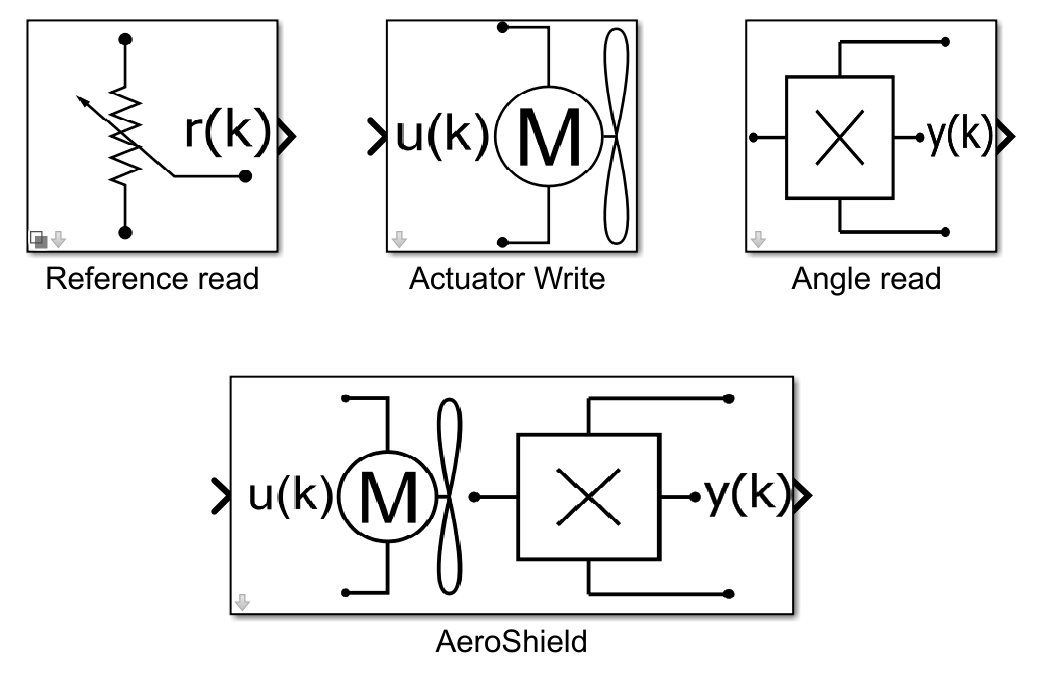
\includegraphics[width=125mm]{obr/AeroLib.png}
	\caption{Knižnica AeroLibrary.}\label{OBRAZOK 2.6.4}
\end{figure}

Blok \verb|Actuator Write| má najjednoduchšiu vnútornú štruktúru. Skladá sa z funkcie \verb*|Constrain|, ktorá prepočíta percentuálnu hodnotu vstupu na výstupný 8-bitový PWM signál. Tento signál posiela na Shield blok \verb*|PWM|, z knižnice \textit{Simulink Support Package for Arduino Hardware}. 

\subsubsection{Reference read}
\label{AngleRead}

V časti \verb|Reference read| máme na výber možnosť manuálnej, alebo automatickej trajektórie. Používateľ si z týchto možností vyberie pomocou tlačidiel v maske bloku. Vnútorná štruktúra sa ďalej skladá z troch podsystémov, z ktorých dva, pre manuálnu trajektóriu obr.\ref{OBRAZOK 2.6.5}, sú takmer totožné. Rozdiel medzi nimi je taký, že pri použití niektorých druhov Arduina\footnote[11]{Due, MKR1000, MKR1010, MKRZero, Nano 33IoT.} je pri použitý bloku \verb|Analog input|, výstup v tvare 12-bitového čísla, narozdiel od 10-bitového, ako je tomu pri ostatných podporovaných modeloch Arduina. Načítaná hodnota je ďalej upravovaná do percentuálnej podoby, pomocou prenásobenia konštantou v bloku \verb*|gain|. 

Podsystém pre automatickú trajektóriu obr.\ref{OBRAZOK 2.6.66} má viacero možností nastavenia. Ponúka možnosť zmeny pola referenčnej trajektórie, dĺžku trvania jednotlivých sekcií ako aj zmenu vzorkovacieho času. Viac informácií o bloku \verb|Reference read| nájdeme v časti \ref{Maska} na strane \pageref{Maska}. 

\begin{figure}[!tbh]
	\hfill
	\subfigure[Tri podsystémy bloku Reference read.]{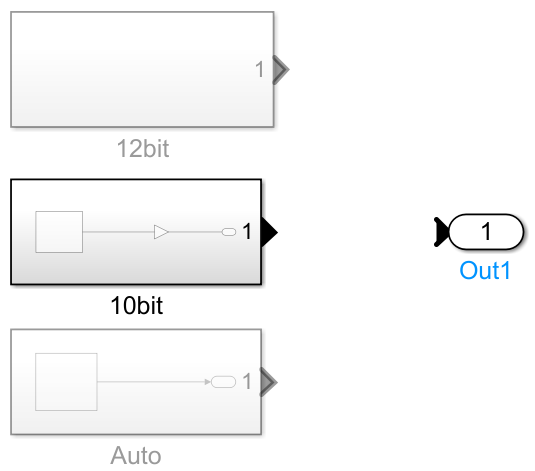
\includegraphics[width=6cm]{obr/Subsystem.png}}
	\hfill
	\subfigure[Podsystém pre 10-bitovú logiku.]{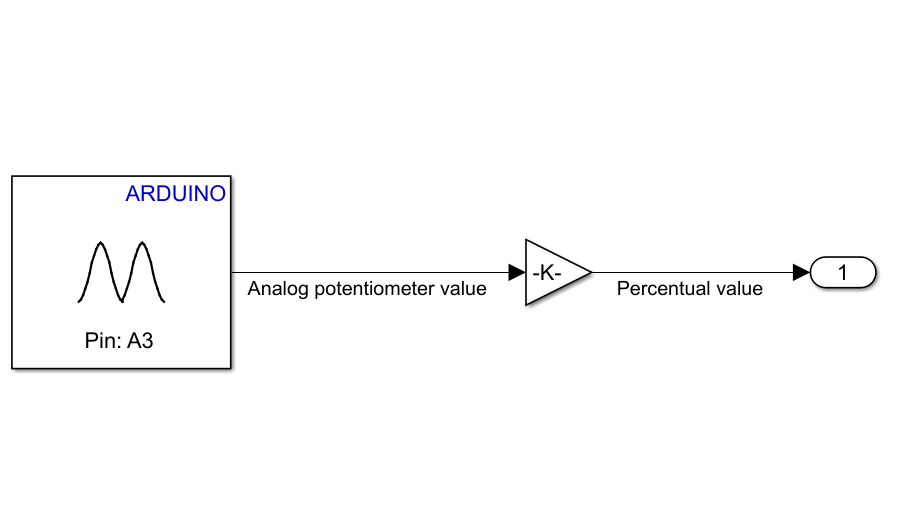
\includegraphics[width=9cm]{obr/10bit.png}}
	\hfill
	\caption{Reference read- Simulink.}\label{OBRAZOK 2.6.5}
\end{figure}

V \verb|MATLAB function| bloku, ktorý sa nachádza v podsystéme pre automatickú trajektóriu, nájdeme kód \ref{vrku}. Funguje na veľmi podobnom princípe ako v príklade \ref{matlabik}. Tento funkčný blok má 4 vstupy, z ktorých 3 zadávame v maske bloku a 2 výstupy. Funkcia kontroluje čas, ako dlho sú spustené jednotlivé úseky automatickej trajektórie. Robí tak pomocou bloku \verb|Clock|, ktorý udáva aktuálny čas od spustenia simulácie. Pokiaľ je úsek trajektórie spustený dlhšie ako zadávame v maske bloku, funkcia automaticky prejde na ďalší úsek. Pokiaľ bola automatická trajektória ukončená, funkcia zastaví prebiehajúcu simuláciu. 



\begin{lstlisting}[caption={MATLAB function blok autiomatická trajektoria.},captionpos=b, label=vrku]
function [r, stopFlag] = fcn(clock, refVector, sectionLength, Ts)
persistent counter;
pauseTime = 2;

if isempty(counter)
counter = 1;
end
if clock > pauseTime
RefLength = length(refVector);
SectionDuration = sectionLength * Ts;
if (clock - pauseTime) <= (SectionDuration * counter)
r = refVector(counter);
stopFlag = 0;
else
counter = counter + 1;
if counter <= RefLength
r = refVector(counter);
stopFlag = 0;
else
r = refVector(counter-1);
stopFlag = 1; 
end
end
else
r = refVector(1);
stopFlag = 0;
end
end
\end{lstlisting}

\begin{figure}[!tbh]
	\centering
	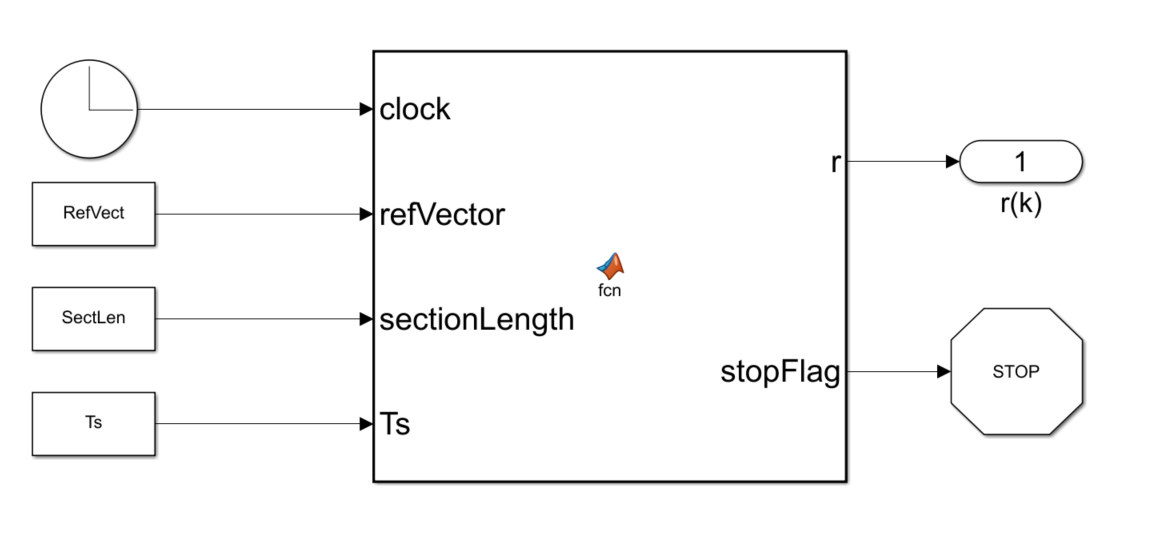
\includegraphics[width=100mm]{obr/AutoSimul.png}
	\caption{Automatická trajektória- Simulink.}\label{OBRAZOK 2.6.66}
\end{figure}

\subsubsection{Angle read}

Tento blok obr.\ref{OBRAZOK 2.6.6} slúži na čítanie uhlu kyvadla, ako aj pre bezpečnostnú kontrolu uhlu kyvadla. Jeho vnútorná štruktúra sa dá rozdeliť na štyri menšie celky: 
\begin{itemize}
	\item zapisovanie príkazov na senzor,  
	\item čítanie uhlu kyvadla zo senzoru, 
	\item kalibrácia nulového uhlu kyvadla,
	\item kontrola uhlu kyvadla. 
\end{itemize}

\begin{figure}[!tbh]
	\centering
	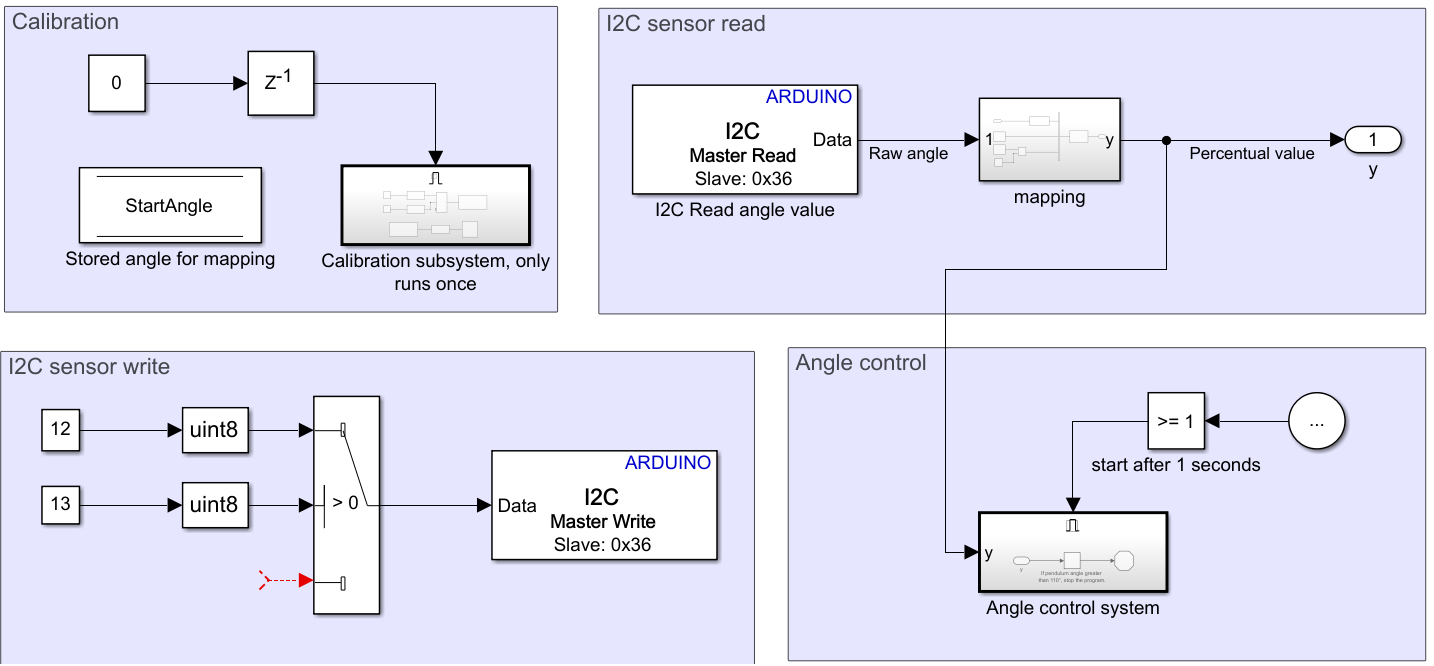
\includegraphics[width=\textwidth]{obr/AngleRead.png}
	\caption{Angle read- Simulink.}\label{OBRAZOK 2.6.6}
\end{figure}


\paragraph{I2C zápis}

Blok I2C Write obr.\ref{OBRAZOK 2.6.6}(ľavý dolný roh), z knižnice \textit{Simulink Support Package for Arduino Hardware}, zapisuje na senzor striedavo hodnoty 12 a 13, ktoré slúžia ako príkaz pre čítanie a následné odoslanie hodnoty pootočenia kyvadla. Prepínanie medzi týmito dvomi hodnotami zabezpečuje automatický prepínač (Automatic switch). 

\paragraph{I2C čítanie}

Samotné čítanie uhlu zabezpečuje blok I2C Read obr.\ref{OBRAZOK 2.6.6}(pravý horný roh), ktorého výstupom je 12-bitové číslo, predstavujúce aktuálne natočenie kyvadla. Tento výstup musíme previesť na uhlovú výchylku v rozmedzí od 0 do 360°. Tento prevod sa vykonáva v mapovacom podsystéme obr.\ref{OBRAZOK 2.6.7}. Mapovanie funguje na rovnakom princípe ako v príklade \ref{MatlabPID}. Jednotlivé premenné vchádzajú do bloku \verb*|MUX|, ktorý slúži ako multiplexer\footnote[12]{Zariadenie, ktoré vyberá medzi viacerými analógovými alebo digitálnymi vstupnými signálmi a tieto preposiela na jednu výstupnú linku.}. Signál z multiplexoru vstupuje do \verb|fcn bloku|, ktorý prepája Simulink s MATLABOM. Zdrojový kód \ref{MAPfcn} zobrazuje funkciu vo vnútri tohoto bloku. 


\begin{figure}[!tbh]
	\centering
	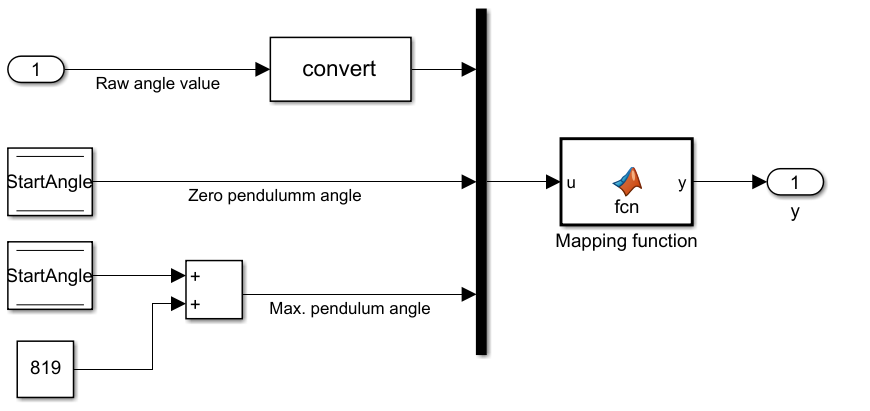
\includegraphics[width=\textwidth]{obr/SensMap.png}
	\caption{Mapovanie uhlu kyvadla- Simulink.}\label{OBRAZOK 2.6.7}
\end{figure}


\begin{lstlisting}[caption={Mapovacia funkcia vo fcn bloku.},captionpos=b,label=MAPfcn]
	function y = fcn(u)
	angMin=0;
	angMax=72;
	y = ((u(1) - u(2)) * (angMax - angMin)) / (u(3) - u(2)) + angMin ;
\end{lstlisting}


Proces získania premennej \verb|StartAngle|, ktorú využívame pri mapovaní, je opísaný v nasledujúcom odstavci. 

\paragraph{Kalibrácia} 
Kalibrácia prebieha vždy len raz a to pri spustení simulácie. V podsystéme (Enabled Subsystem) obr.\ref{OBRAZOK 2.6.8}.a, ktorý je spustený len ak je do neho privedený signál, sa nachádzajú funkcie pre zapisovanie a čítanie informácii zo senzoru. Uhol ktorý je týmto podsystémom zaznamenaný pri spustený simulácie, sa uloží v bloku \verb|Data store Write|, ako premenná \verb|StartAngle| obr.\ref{OBRAZOK 2.6.8}.b.                                                                                                                                                                                                                                                                                                                                                                                                                                                                                                                                                                                                                                                                                                                                                                                                                                                                                                                                                                                                                                                                                                                                                                                                                                                                                                                                                                                                                                                                                                                                                                                                                                                                                                                                                                                                                                                                                                                                                                                                                                                                                                                                                                                                                                                                                                                                                                                                                                                                                                                                                                                                                                                                                                                                                                                                                                                                                                                                                                                                                                                                                                                                                                                                                                                                                                                                                                                                                                                                                                                                                                                                                                                                                                                                                                                                                                                                                                                                                                                                                                                                                                                                                                                                                                                                                                                                                                                                                                                                                                                                                                                                                                                                                                                                                                                                                                                                                                                                                                                                                                                                                                                                                                                                                                                                                                                                                                                                                                                                                                                                                                                                                                                                                                                                                                                                                                                                                                                                                                                                                                                                                                                                                                                                                                                                                                                                                                                                                                                                                                                                                                                                                                                                                                                                                                                                                                                                                                                                                                                                                                                                                                                                                                                                                                                                                                                                                                                                                                                                                                                                                                                                                                                                                                                                                                                                                                                                                                                                                                                                                                                                                                                                                                                                                                                                                                                                                                                                                                                                                                                                                                                                                                                                                                                                                                                                                                                               

\begin{figure}[!tbh]
	\hfill
	\subfigure[Sústava pre zabezpečenie kalibrácie.]{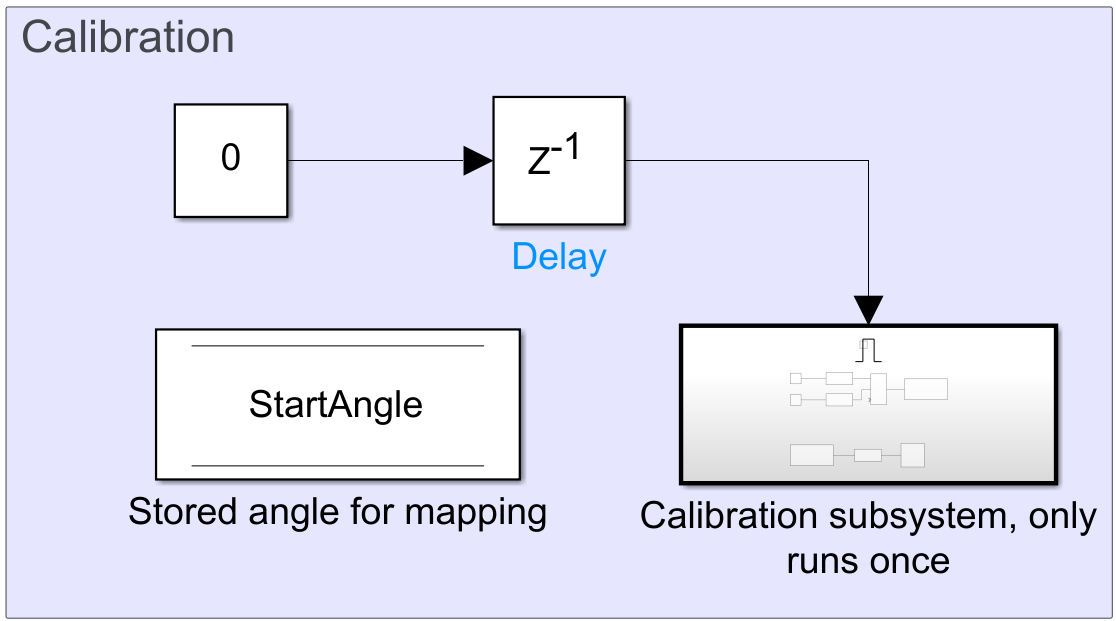
\includegraphics[width=6cm]{obr/Calibrat.png}}
	\hfill
	\subfigure[Podsystém pre zaznamenanie nulového uhla.]{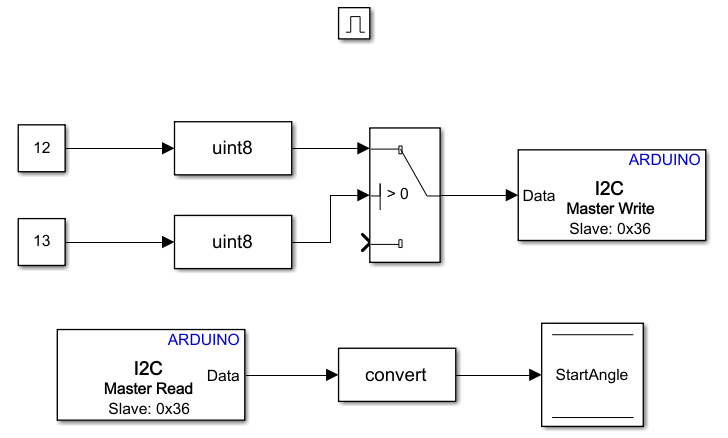
\includegraphics[width=9cm]{obr/calibDnu.png}}
	\hfill
	\caption{Kalibrácia- Simulink.}\label{OBRAZOK 2.6.8}
\end{figure}

\paragraph{Kontrola uhlu}

Kontrola uhlu kyvadla prebieha v podsystéme, ktorý je spustený päť sekúnd po začatí simulácie obr.\ref{OBRAZOK 2.6.6}(pravý dolný roh). Časový posun je použitý z dôvodu občasného šumu premenných počas začiatku simulácie. Tento šum môže spôsobiť nechcené výkyvy hodnoty uhlu kyvadla, ktoré by splnili podmienku v podsystéme a tým by zastavili priebeh simulácie. V podsystéme obr.\ref{OBRAZOK 2.6.9}, sa nachádza blok \verb|Compare To Constant|, ktorý porovnáva hodnotu uhlu kyvadla, s daným maximálnym uhlom kyvadla. Táto hodnota je v našom prípade 110°. Pokiaľ kyvadlo dosiahne väčší uhol, ako je uhol dovolený, blok \verb|Stop Simulation| zastaví simuláciu.  

\begin{figure}[!tbh]
	\centering
	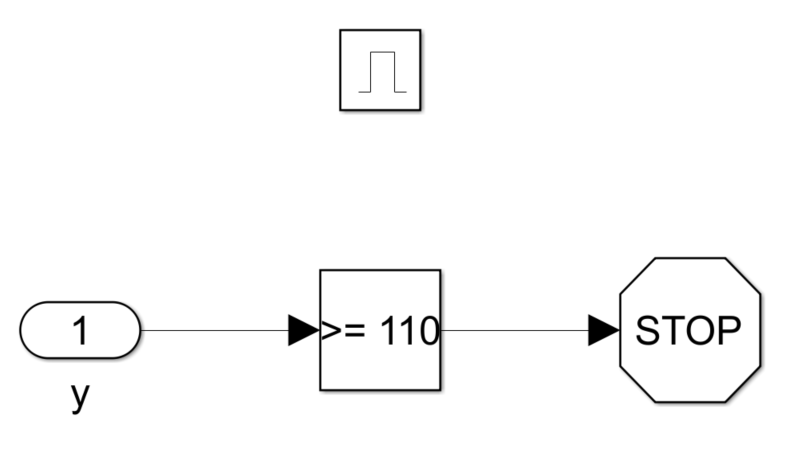
\includegraphics[width=100mm]{obr/AngleControl.png}
	\caption{Podsystém na kontrolu uhlu kyvadla.}\label{OBRAZOK 2.6.9}
\end{figure}

\newpage
\subsubsection{Tvorba masky}
\label{Maska}

Maska slúži ako vlastné používateľské rozhranie bloku resp. podsystému. Maskovaním bloku zapúzdrime blokovú schému tak, aby mala podla potreby, vlastné dialógové okná s nastaviteľnými parametrami, popisy bloku, výzvy na zadanie parametrov alebo texty s nápovedami. Vďaka maske blokov, sa tieto viacej podobajú na bloky, ktoré nájdeme v predprogramovaných knižniciach Simulinku. Masku upravujeme pomocou editora, ktorý spustíme pravým kliknutím na blok, s následným výberom možnosti \verb|Mask|. V maske sa nachádzajú štyri hlavné editovacie rozhrania. 

Prvým z nich je záložka \verb|Icon & Ports|. V tomto okne upravujeme vzhľad bloku. Teda jeho zobrazenie, rotáciu, inicializáciu, alebo ikonu bloku. Pre všetky bloky v knižnici AeroLibrary, boli vytvorené vlastné ikony, ktoré sa do masky vkladajú príkazom \code{image('assets/Pote.png')}.

Ďalšou v poradí je záložka \verb|Parameters & Dialog|. V tejto sekcii nastavujeme vzhľad a funkcie masky, ktorá sa zobrazí po kliknutí na blok. V prípade bloku \verb|Reference read|, máme v maske na výber voľbu automatickej alebo manuálnej referenčnej trajektórie. Medzi týmito možnosťami si vyberáme pomocou tlačidiel (Radio button) obr.\ref{OBRAZOK 2.6.100}, ktorých výber taktiež formátuje zobrazenie masky bloku. 

Pokiaľ si z tlačidiel vyberieme manuálnu trajektóriu, zobrazí sa ďalšia možnosť výberu, a tou je model dosky Arduino. Jedná sa o roletové, alebo "popup$"$ menu, v ktorom si vyberieme typ dosky s ktorou používame AeroShield. Dôvod tohoto výberu je opísaný v časti \ref{AngleRead}, na strane \pageref{AngleRead}. Pokiaľ si zvolíme Automatickú referenčnú trajektóriu, možnosť voľby dosky sa nezobrazí. Namiesto toho sa zobrazia možnosti nastavenia automatickej trajektórie. Táto funkcia je vykonávaná automaticky, zdrojovým kódom \ref{Callback}, ktorý sa nachádza v časti \verb|Callback|, v nastaveniach tlačidiel voľby trajektórie. 

\begin{lstlisting}[caption={Callback funkcia.},captionpos=b,label=Callback]
ref = get_param(gcb,'ref');
if strcmp(ref(1),'M')
set_param(gcb,'MaskVisibilities',{'on';'on';'off';'off';'off';'off'}),
else
set_param(gcb,'MaskVisibilities',{'on';'off';'on';'on';'on';'on'}),
end
\end{lstlisting}

Pomocou príkazu \verb|get_param|, sa nám do premennej \verb|ref|, uloží výber tlačidla v maske. Príkaz \verb|gcb| vráti cestu
daného bloku v aktuálnom systéme. Podmienka \verb|if| kontroluje ktorú z možností sme si vybrali, pomocou príkazu \verb|strcmp|, ktorý porovnáva prvé písmeno z premennej \verb|ref|, s písmenom 'M' (Manual). Pokiaľ sa tieto zhodujú, príkaz \verb|set_param|, spolu s príkazom \verb|MaskVisibilities|, nastaví polia tlačidiel ako viditeľné, teda s hodnotou \verb|'on'|. Pokiaľ sa písmená nezhodujú a teda bola vybraná trajektória automatická, možnosť výberu dosky Arduino, je skrytá príkazom \verb|'off'| a namiesto nej, sa zobrazia ďalšie štyri editovateľné polia. 

\verb|Initialization| tvorí tretiu záložku v maske. V tejto záložke môžeme pridávať MATLAB kód, ktorý ovláda a formátuje podsystémy. V maske bloku \verb|Reference read |, máme v tejto záložke vložený kód \ref{Initialization}. Podľa pravdivosti \verb|if| podmienky, príkaz \newline \verb|set_param(gcb,'LabelModeActiveChoice'| aktivuje podsystém bloku, ktorého názov je uvedený ako tretí parameter v zátvorke príkazu. 

\begin{lstlisting}[caption={Initialization- maska Reference read.},captionpos=b,label=Initialization]
	ref = get_param(gcb,'ref');
	model = get_param(gcb,'model');
	if strcmp(ref,'Manual')
	if strcmp(model,'Due')
	set_param(gcb,'LabelModeActiveChoice', '12bit');
	elseif strcmp(model,'MKR1000')
	set_param(gcb,'LabelModeActiveChoice', '12bit');
	elseif strcmp(model,'MKR1010')
	set_param(gcb,'LabelModeActiveChoice', '12bit');
	elseif strcmp(model,'MKRZero')
	set_param(gcb,'LabelModeActiveChoice', '12bit');
	elseif strcmp(model,'Nano 33IoT')
	set_param(gcb,'LabelModeActiveChoice', '12bit');
	elseif strcmp(model,'Others') 
	set_param(gcb,'LabelModeActiveChoice', '10bit');
	end
	end
	if strcmp(ref,'Automatic')
	set_param(gcb,'LabelModeActiveChoice', 'Auto');
	end
\end{lstlisting}


\begin{figure}[!tbh]
	\centering
	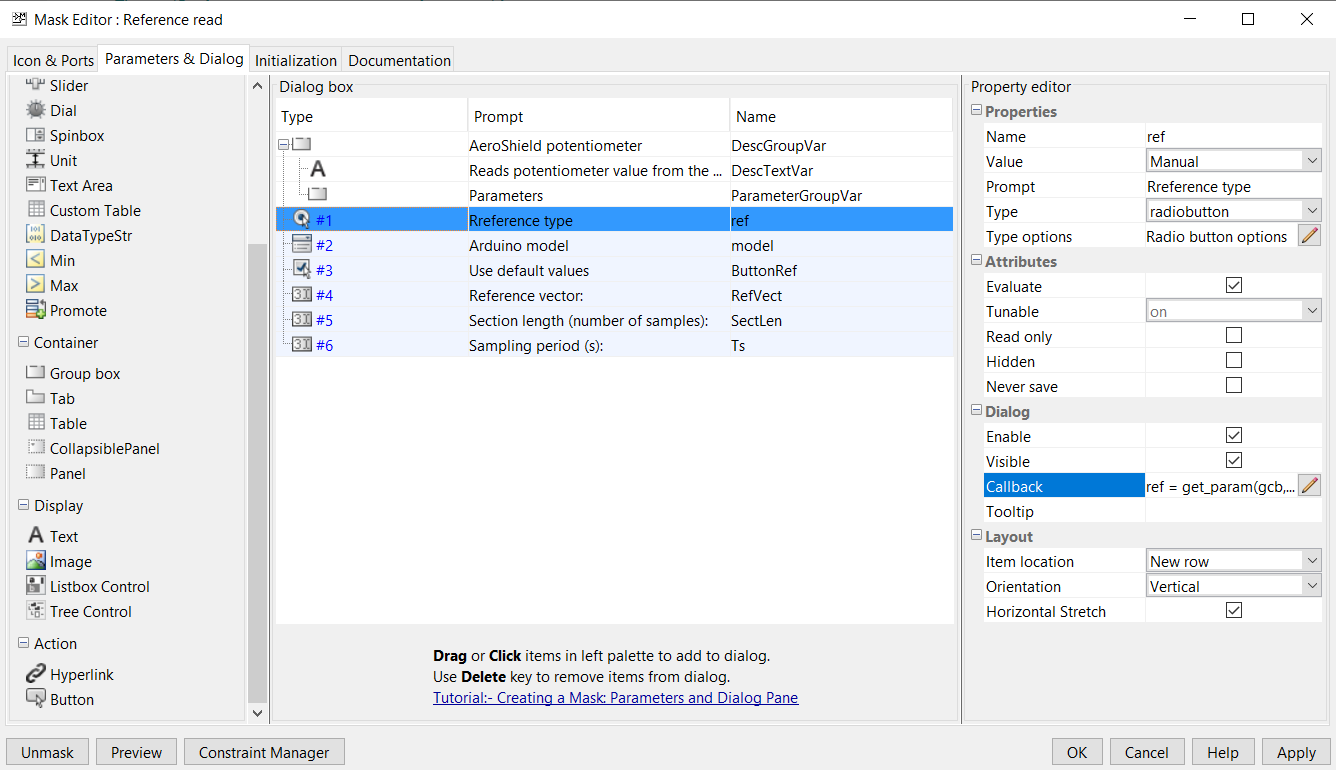
\includegraphics[width=\textwidth]{obr/ParamAnd.png}
	\caption{Nastavenia parametrov masky bloku Reference read.}\label{OBRAZOK 2.6.101}
\end{figure}


\begin{figure}[!tbh]
	\hfill
	\subfigure[Nastavenia masky pri výbere manuálnej trajektórie.]{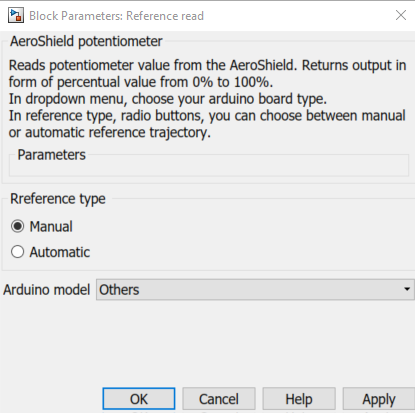
\includegraphics[width=7.3cm]{obr/Maska.png}}
	\hfill
	\subfigure[Zobrazenie masky pri výbere automatickej trajektórie.]{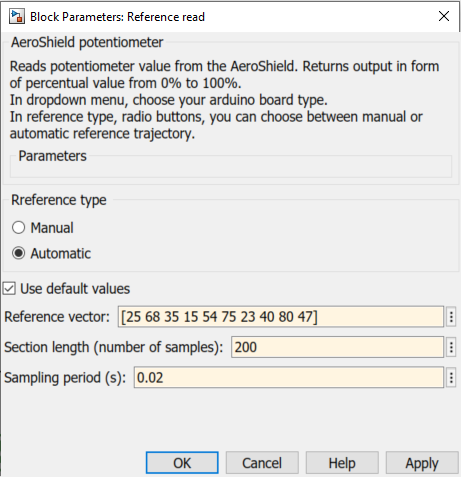
\includegraphics[width=7cm]{obr/MaskaA.png}}
	\hfill
	\caption{Reference read- Simulink.}\label{OBRAZOK 2.6.100}
\end{figure}



Pre lepšie porozumenie blokov a ich funkcií, bol v API Simulink zostavený inštruktážny príklad \verb|AeroShieldOpenLoop| obr.\ref{OBRAZOK 2.6.111}. Tento príklad funguje na princípe merania hodnoty bežca potenciometra na Shielde, a následného zapisovania nameranej hodnoty na akčný člen sústavy. Zároveň je meraný uhol v ktorom sa kyvadlo nachádza. Obe tieto hodnoty sú priebežne zobrazované na grafe. 

\begin{figure}[!tbh]
	\centering
	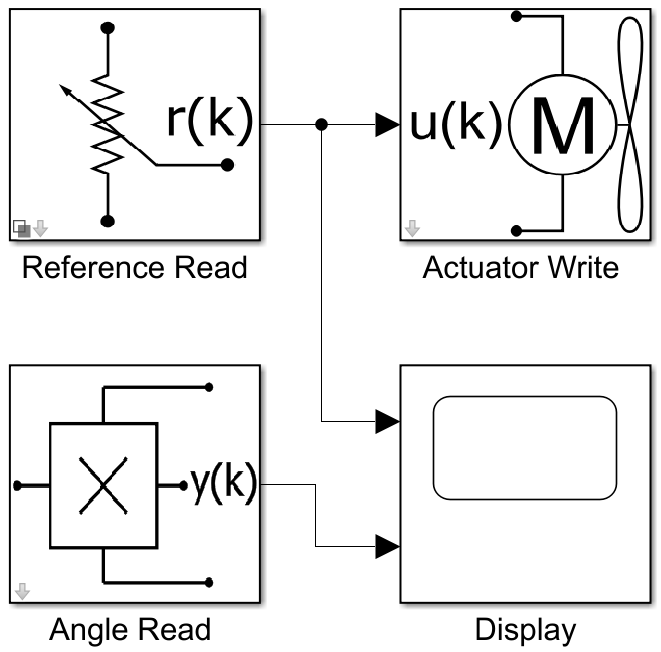
\includegraphics[width=100mm]{obr/AeroOpenLoop.png}
	\caption{AeroShield\_OpenLoop.}\label{OBRAZOK 2.6.111}
\end{figure}


\chapter{Didaktické príklady}
\label{Didaktické príklady}

Pre AeroShield bolo v prostredí Arduino IDE, MATLAB a Simulink vytvorených niekoľko vzorových programov, ktoré demonštrujú všetky jeho funkcie. Programy sú rozdelené do dvoch veľkých skupín, konkrétne programy v otvorenej slučke bez spätnej väzby a programy v uzavretej slučke so spätnou väzbou. 

Ich rozdiel spočíva v tom, že pri riadení bez spätnej väzby, hovoríme o ovládaní systému, kedy sa snažíme dosiahnuť žiadané hodnoty výstupov bez spätnej informácie o vykonaní procesu, alebo o jeho hodnote. V prípade riadenia so spätnou väzbou sa jedná o reguláciu. Pri regulácii sa kontroluje bezprostredný účinok riadenia, ktorý sa porovnáva so žiadanou hodnotou výstupu a na vyrovnanie ich vzájomnej chyby, sa okamžite vykonáva zásah do vstupných veličín. 

\section{Programy v otvorenej slučke, bez spätnej väzby}
\subsection{Arduino IDE}
\label{bezspatnej}

Ako prvý príklad si ukážeme program s názvom \verb|AeroShield_OpenLoop.ino| napísaný v prostredí Arduino IDE. Hlavnou ideou tohoto programu je jednoduché ovládanie otáčok motorčeka, pomocou potenciometra. Na začiatku programu inicializujeme hlavnú knižnicu AeroShieldu pomocou príkazu \verb|#include "AeroShield.h"|. Následne deklarujeme premenné, ktorých hodnoty budú vypisované na sériový monitor. 

\begin{lstlisting}[caption={AeroShield open loop dekleracia.},captionpos=b]
	float startangle=0;           //  Premenna pre nulovy uhol
	float lastangle=0;            //  Premenna pre maximalny uhol 
	float pendulumAngle;          //  Uhol natocenia kyvadla
	float referencePercent;       //  Hodnota potenciometra
	float CurrentMean;	      //  Hodnota prudu odoberaneho motorom 
\end{lstlisting}

V časti \verb|setup()| ako prvé prebehne nastavenie rýchlosti sériovej komunikácie \verb|Serial.begin(115200)|. Číslo 115 200 predstavuje počet zmien, stavu z 0 na 1 resp. zo stavu high na stav low, za sekundu. Toto tempo signálnej rýchlosti nazývame \verb|baud rate|. Nasleduje funkcia \verb|AeroShield.begin()|, ktorá sleduje prítomnosť magnetu, a prednastaví potrebné premenné a funkcie pinov. Poslednou funkciou je kalibrácia kyvadla \verb|AeroShield.calibration()|, spolu s výpočtom začiatočného a koncového uhla kyvadla. 

\begin{lstlisting}[caption={AeroShield open loop setup().},captionpos=b]
	void setup() {                // Setup prebehne len jeden krat 
		Serial.begin(115200);       // Zaciatok seriovej komunikacie 
		AeroShield.begin();  // Inicializacia AeroShieldu 
		startangle = AeroShield.calibration(AeroShield.getRawAngle());   // Kalibracia kyvadla
		lastangle=startangle+1024;  // Kalkulacia uhlu kyvadla pre map function
	}
\end{lstlisting}

V cykle \verb|loop()| prebehne ako prvé mapovanie uhlu kyvadla pomocou funkcie \newline\verb|AutomationShield.mapFloat()|. Nasleduje čítanie hodnoty potenciometra, ktorá slúži na ovládanie akčného člena pomocou funkcie \verb|AeroShield.actuatorWrite()|. Na sériový súradnicový zapisovač sa modrou farbou vykreslí uhol kyvadla, červenou farbou hodnota potenciometra a zelenou veľkosť prúdu odoberaného motorom obr.\ref{OBRAZOK 3.1}. 

\begin{lstlisting}[caption={AeroShield open loop loop().},captionpos=b]
	void loop() {
		referencePercent= AeroShield.referenceRead();  // Citanie potenciometra
		AeroShield.actuatorWrite(referencePercent); // Pohyb akcneho clenu
		CurrentMean= AeroShield.currentMeasure();  // Meranie prudu
		
		Serial.print(pendulumAngle);    
		Serial.print(" ");
		Serial.print(referencePercent);  
		Serial.print(" ");
		Serial.print(CurrentMean);   
		Serial.println(" ");
	}
\end{lstlisting}

\begin{figure}[!tbh]
	\centering
	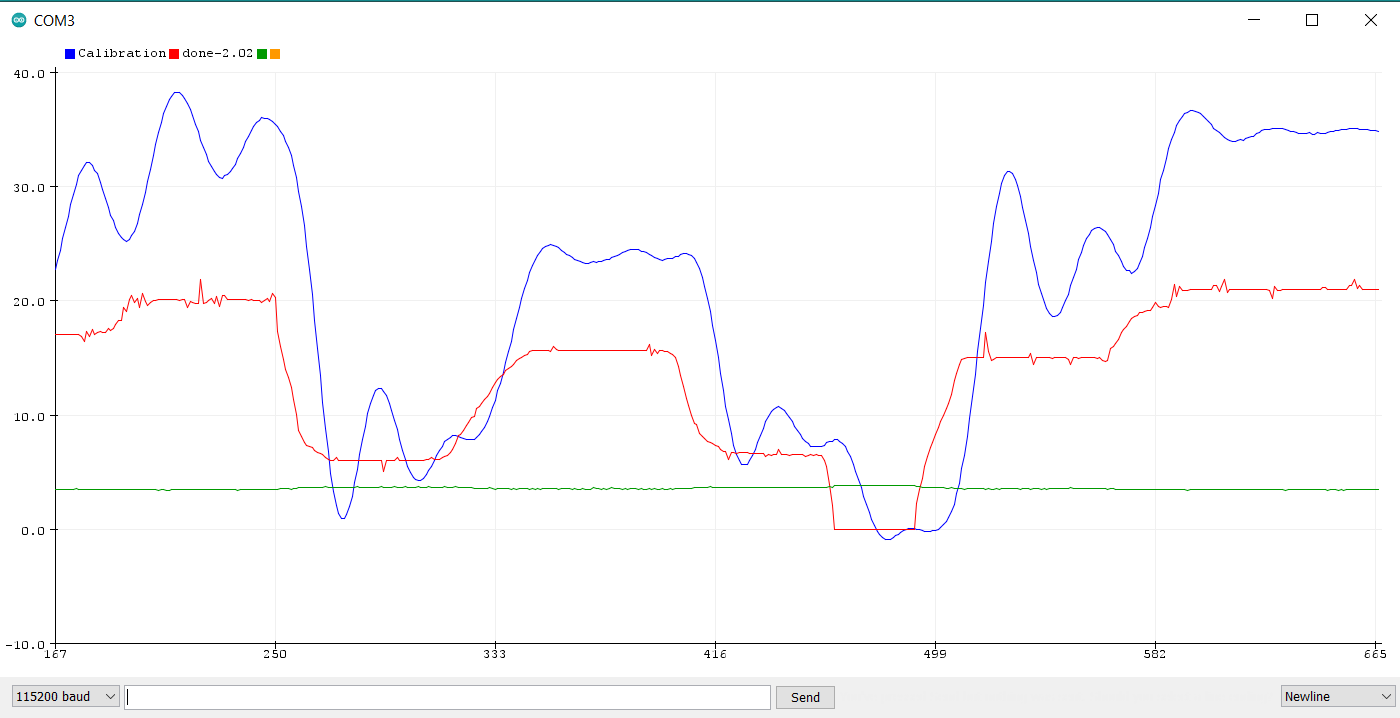
\includegraphics[width=120mm]{obr/VystupOLIDE.png}
	\caption{Výstup z programu AeroShieldOpenLoop.ino.}\label{OBRAZOK 3.1}
\end{figure}

\newpage
\subsection{MATLAB}
\label{MatlabPID}

V príklade \verb|AeroShieldOpenLoop.m| si ukážeme výhody a možnosti zobrazovania výstupov, v prostredí MATLAB. 

Na začiatku kódu vymažeme všetky premenné a objekty pomocou série príkazov \code{Clear all, clc}. Následne načítame knižnicu AeroShieldu a vykonáme funkciu \verb|AeroShield.begin()|. Kód pokračuje kalibráciou nulového uhlu kyvadla, zadefinovaním premenných na počítanie času, ako aj premenných na ukladanie hodnôt potenciometra a uhlu kyvadla. 

\begin{lstlisting}[caption={AeroShield open loop inicializacia.},captionpos=b]
	% vymazanie premennych a objektov 
	clear all
	clc 
	
	% nacitanie kniznice AeroShieldu  
	AeroShield=AeroShield;
	% vytvorenie objektov arduino, as5600
	AeroShield.begin();
	% kalibracia
	startangle= AeroShield.calibration(); 
	lastangle=startangle+2048; 
	
	% premenne na pocitanie casu
	time = 0;
	count = 0;
	angle = 0;          % uhol kyvadla
	potentiometer = 0;  % hodnota potenciometra
\end{lstlisting}

Nasleduje while cyklus, ktorý je ukončený zatvorením vykresľovaného grafu. V cykle najskôr čítame hodnotu potenciometra pomocou príkazu \verb|AeroShield.referenceRead()| a túto hodnotu zapisujeme na akčný člen príkazom \verb| AeroShield.actuatorWrite()|. Pokračujeme čítaním uhlu kyvadla \verb|AeroShield.getRawAngle()|, za ktorým prebehne mapovanie premennej z hodnoty raw na stupne. Premenná \verb|count| slúži na počítanie počtu prejdených cyklov, na tvorbu usporiadaného radu premenných, ako aj na vykresľovanie pohyblivej x-ovej osi grafu obr.\ref{OBRAZOK 3.2}. Ľavá stupnica grafu je stacionárna a zobrazuje hodnotu potenciometra, pravá stupnica zobrazuje uhol kyvadla v stupňoch a svoje rozpätie zväčšuje, alebo zmenšuje v závislosti na výchylke kyvadla. Na konci programu ešte nájdeme if podmienku, ktorá kontroluje uhol kyvadla, ktorý ak nadobudne hodnotu väčšiu ako 110°, proces sa automaticky ukončí a vypíše sa upozornenie. Posledný príkaz \verb|clear AeroShield.arduino| vymaže objekt \verb|arduino| a pripraví MATLAB na spustenie ďalšieho programu. 

\begin{lstlisting}[caption={AeroShield open loop, while cyklus.},captionpos=b]
	while ishandle(plotGraph)           % slucka bezi pokial sa nezatvori graf
	
	pwm = AeroShield.referenceRead();   % citanie hodnoty potenciometra
	AeroShield.actuatorWrite(pwm);      % zapis na aktuator
	RAW= AeroShield.getRawAngle();      % citanie raw uhlu
	angle_ = mapped(RAW, startangle, lastangle, 0, 180); % mapovanie raw uhol na stupne
	
	count = count + 1;                              % zaznamenavanie poctu cyklov
	time(count) = toc;                              % zaznamenavanie casu
	angle(count) = angle_(1);                       % hodnota uholu v case 
	percenta= mapped(pwm, 0.0, 5.0, 0.0, 100.0);    % mapovanie pwm na percenta
	potentiometer(count) = percenta(1);             % hodnota potenciometra v case
	set(plotGraph,'XData',time,'YData',angle);      % vykresli prve data
	set(plotGraph1,'XData',time,'YData',potentiometer); % vykresli druhe data  
	axis([time(count)-5 time(count) 0 100]);        % ,,beziaca" x-ova osa
	
	if (angle_ > 110)                            % ak uhol kyvadla vacsi ako 110 stupnov 
	AeroShield.actuatorWrite(0.0);      % zastav motor  
	disp('Angle of pendulum too high. AeroShield is turned off')
	break                               % zastav program
	end
	end  
	
	clear AeroShield.arduino;           
\end{lstlisting}

\begin{figure}[!tbh]
	\centering
	\includegraphics[width=\textwidth]{obr/ASOLmat.png}
	\caption{Výstup z programu AeroShieldOpenLoop.m.}\label{OBRAZOK 3.2}
\end{figure}

\subsection{Simulink}


Na ukážku funkcií jednotlivých blokov \verb|AeroLibrary|, bol v API Simulink zostavený inštruktážny príklad \verb|AeroShieldOpenLoop| obr.\ref{OBRAZOK 2.6.111}. V tomto príklade sa pomocou hodnoty potenciometra ovláda akčný člen. Zároveň je meraný uhol, v ktorom sa kyvadlo nachádza a obe tieto hodnoty sú priebežne zobrazované na grafe pomocou bloku \verb|Scope|. 

\begin{figure}[!tbh]
	\centering
	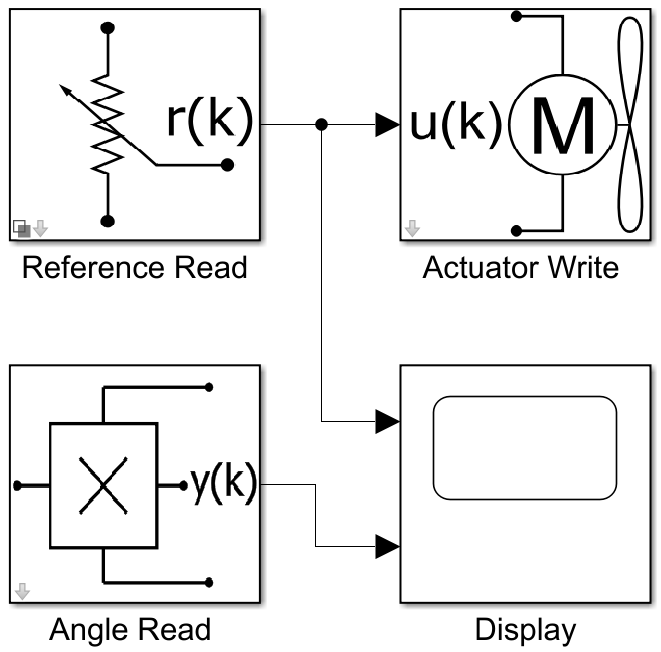
\includegraphics[width=100mm]{obr/AeroOpenLoop.png}
	\caption{AeroShield\_OpenLoop.}\label{OBRAZOK 2.6.111}
\end{figure}



\chapter{PID regulácia}
\label{PIDPID}

PID reguláciu sme si vybrali z dôvodu jednoduchosti použitia, ako aj z dôvodu že práve PID regulácia je vyučovaná medzi prvými v rámci teórie riadenia. P, PI alebo PID regulátory taktiež patria medzi veľmi populárne typy riadiacich algoritmov.  

Skôr ako si ukážeme príklady s využitím PID regulátora, musíme si vysvetliť ako PID regulátor funguje. Základom je získavanie informácii o sledovanej resp. riadenej veličine, za pomoci senzoru a jej porovnávanie s hodnotou žiadanou. Vďaka tomu, že získavame informácie o výstupe, ktoré aktívne využívame na riadenie akčného člena, môžeme hovoriť o spätnoväzbovom riadení. Spätnoväzbové riadenie, je teda také riadenie, ktoré ovplyvnuje sústavu na základe aktuálne získaných informácii o stave, v ktorom sa sústava nachádza. Pri takomto riadení existuje množstvo algoritmov, ktoré ovládajú správanie sa systému. Medzi tieto algoritmy patrí napríklad: Lineárne riadenie s premenlivým parametrom (LPV), Lineárno-kvadratické riadenie (LQ), Modelové prediktívne riadenie (MPC), Proporcionálno-integračno-derivačné riadenie (PID)...

PID regulátor obr.\ref{OBRAZOK 3.3}, ovplyvňuje akčné zásahy do sústavy \verb|u(t)| na základe zaznamenaných výstupných informácii \verb|y(t)|. Veľkosť akčného zásahu \verb|u(t)| vypočítame na základe rozdielu medzi požadovanou hodnotou \verb|w(t)| a hodnotou reálnou \verb|y(t)|. Tento rozdiel označujeme tiež ako regulačná odchýlka \verb|e(t)|. Písmeno $"$t$"$ v zátvorkách predstavuje, časovú závislosť premenných. 

\begin{figure}[!tbh]
	\centering
	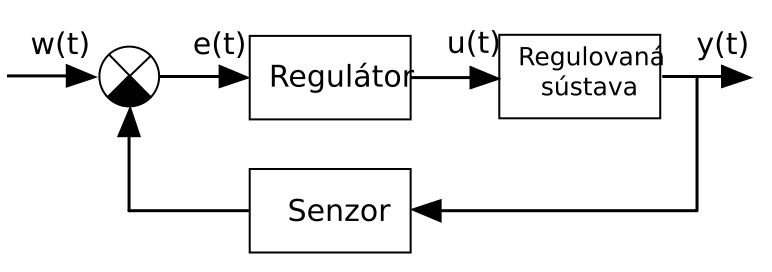
\includegraphics[width=120mm]{obr/pid.png}
	\caption{Schéma riadenia PID regulátorom.}\label{OBRAZOK 3.3}
\end{figure}

Skratka PID je zložená zo začiatočných písmen zložiek, z ktorých sa regulátor skladá. 

\begin{itemize}
	\item \textbf{P}- označuje tzv. proporcionálnu zložku. Akčný zásah \verb|u(t)|, je priamo úmerný veľkosti regulačnej odchýlky \verb|e(t)|. K$_p$ predstavuje proporcionálnu konštantu, ktorou násobíme regulačnú odchýlku na získanie požadovaného vstupu rov.\ref{rovnicajedna}. 
	\begin{align}
		\label{rovnicajedna}
		u(t)=K_p e(t)
	\end{align}
	Konštanta K$_p$ je veľmi dôležitou pri nastavovaní parametrov PID regulátora. Zvyšovaním hodnoty proporcionálnej zložky znižuje regulačnú odchýlku, avšak nikdy nedosiahneme úplne odstránenie trvalej regulačnej odchýlky. Zmenou proporcionálnej zložky vieme taktiež urýchliť, alebo spomaliť nábeh na požadovanú hodnotu. Pre malé hodnoty K$_p$ je nábeh pomalý, a regulačná odchýlka veľká. Pri zvyšovaní hodnoty K$_p$ sa zrýchľuje nábeh, no zároveň narastá nežiadúce kmitanie sústavy. Zvyšovanie hodnoty K$_p$ má svoj limit, za ktorým sa sústava dostáva za hranicu stability a ďalšia regulácia nie je možná. 
	
	\item \textbf{I}- predstavuje integračnú zložku. Integrálny riadiaci člen je priamo úmerný veľkosti chyby, ako aj dobe jej trvania. Pokiaľ má regulovaná veličina menšiu hodnotu ako je požadovaná, integrálna časť PID sa zväčšuje. Naopak pokiaľ je hodnota regulovanej veličiny väčšia ako požadovaná, integrálna časť PID klesá. Pri použití integračnej zložky PID regulátora, bude trvalá regulačná odchýlka nulová\cite{PIDcko}. Čím nižšia bude hodnota T$_i$ rov.\ref{rovnicatriapol}, tým rýchlejšie sa bude výstup približovať žiadanej hodnote, no zároveň však bude narastať kmitanie sústavy.   
	\begin{align}
		\label{rovnicadva}
		u(t)=K_i  \int_{0}^{t} e(\tau)d\tau  
	\end{align}
	\begin{align}
	\label{rovnicatriapol}
        T_i = \dfrac{K_p}{K_i}
    \end{align}
	
	\item \textbf{D}- reprezentuje derivačnú zložku, ktorá predpovedá správanie sa systému, pomocou derivácie regulačnej odchýlky v čase. Rýchlosť zmeny je následne prenásobená derivačnou konštantou K$_d$. Vstup je počítaný podľa rov.\ref{rovnicatri}. Zvyšovanie derivačnej zložky PID regulátora tlmí kmitanie sústavy. Ak však zvolíme derivačnú konštantu priveľkú, kmitanie začne znova narastať\cite{PIDcko}. V praxi sa derivačná zložka veľmi nepoužíva a využívaný je P alebo PI regulátor\cite{1453566}. 
	\begin{align}
		\label{rovnicatri}
		u(t)=K_d  \dfrac{de(t)}{dt}
	\end{align}

\end{itemize}

Pre lepšie chápanie je v tab.\ref{PIDvplyv}\cite{pidcontrol} zhrnutý vplyv jednotlivých zložiek PID, na odozvu systému v uzatvorenej slučke a to pri zvyšovaní hodnoty K$_p$, K$_i$ a K$_d$\footnote[10]{Tabuľka slúži len ako pomôcka pre hrubé ladenia. Jednotlivé zložky PID regulátora, ako aj ich vplyv na sústavu, sú v realite previazané.}. 

\begin{table}[!tbh]
	\begin{tabular}{|c|c|c|c|c|c|}
		\hline
		& Regulačná odchýlka & Rýchlosť ustálenia & Prekmit & Rýchlosť odozvy & Stabilita \\ \hline
		K$_p$                    & znižuje            & malý vplyv         & zvyšuje      & zvyšuje         & znižuje           \\ \hline
		K$_i$                    & znižuje            & znižuje            & zvyšuje      & zvyšuje         & znižuje           \\ \hline
		K$_d$                    & malý vplyv         & zvyšuje            & znižuje      & znižuje         & zvyšuje           \\ \hline
	\end{tabular}
	\caption{Odozva systému na zmenu konštánt.}
	\label{PIDvplyv}
\end{table}

Spojením jednotlivých samostatných zložiek, získame kompletný vzťah pre PID regulátor rov.\ref{rovnicastr}.
\begin{align}
	\label{rovnicastr}
	u(t)=K_p e(t) + K_i  \int_{0}^{t} e(\tau)d\tau + K_d  \dfrac{de(t)}{dt}
\end{align}

\begin{align}
	\label{rovnicapat}
	u(t)=K_p \left(e(t) + \dfrac{1}{T_i}  \int_{0}^{t} e(\tau)d\tau + T_d  \dfrac{de(t)}{dt}\right)
\end{align}
Rovnica \ref{rovnicastr} predstavuje jeden z možných zápisov vzťahu pre PID regulátor. V praxi sa často využíva tvar rov.\ref{rovnicapat}, z dôvodu lepšej interpretácie parametrov, ktoré rovnicu tvoria. T$_i$ predstavuje integračnú a T$_d$ derivačnú časovú konštantu, pričom ich vzťah s konštantami K$_i$ a K$_d$ je v tvare T$_i$ = (K$_p$/K$_i$) a T$_d$ = (K$_d$/K$_p$). Jednotlivé zložky v zátvorke tvoria novú a samostatnú regulačnú odchýlku, ktorá je ešte násobená konštantou K$_p$. Derivačná zložka predpovedá hodnotu regulačnej odchýlky T$_d$ sekúnd(vzoriek) do budúcnosti a integračná zložka sa snaží korigovať súčet hodnoty regulačných odchýlok do T$_i$ sekúnd(vzoriek)\cite{pidcontrol}.

Predchádzajúce rovnice PID regulátorov fungujú pri spojitých procesoch. Avšak pri implementácii PID pomocou číslicových regulátorov, musíme rovnicu transformovať do jej diskrétnej podoby rov.\ref{diskretna}.

\begin{align}
	\label{diskretna}
	u(kT)=K_p \left(e(kT) + \dfrac{T}{T_i} \sum_{i=0}^{k}  e(iT) + \dfrac{T_d}{T} \left[e(kT)-e \left[(k - 1)T\right] \right] \right)
\end{align}

Diskrétna forma PID regulátora je využívaná z toho dôvodu že Arduino resp. počítače nie sú schopné nepretržito zaznamenávať merané hodnoty. Dáta sú preto spracovávané v diskrétnych časových intervaloch \verb|kT|, ktorým hovoríme vzorky. Proces získavania takýchto vzoriek v istej pravidelnom frekvencii, nazývame vzorkovanie. 

Vzorkovanie môže mať rýchlosť niekoľko minút, pri pomaly sa meniacich procesoch, až po mikrosekundy pri procesoch dynamických. Rovnicu v tvare \ref{diskretna} využíva na implementáciu PID regulátora knižnica AutomationShield. 

\section{Programy v uzatvorenej slučke, so spätnou väzbou}
\subsection{Arduino IDE}
\label{sospatnou}
\label{Arduino IDE PID}

V tomto príklade využívame na riadenie PID regulátora, vopred pripravenú knižnicu \verb|PIDAbs|, ktorá je volaná z knižnice \verb|AeroShield|. Za účelom vzorkovania, využívame knižnicu \verb|Sampling|, ktorú načítame do príkladu príkazom \code{#include <Sampling.h>}. Pri voľbe referenčnej trajektórie máme na výber z dvoch možností. Prvou je voľba manuálnej trajektórie, ktorej referenčnú hodnotu nastavujeme pomocou potenciometra na shielde. Druhou voľbou je automatická trajektória, ktorá má vopred naprogramované referenčné hodnoty. Možnosti zadávania trajektórie meníme zmenou hodnoty premennej \verb|MANUAL| z 0 na 1 v príkaze \code{#define MANUAL 0}. Parametre regulátora K$_p$, T$_i$ a T$_d$ slúžia ako symbolické parametre, pre lepší prehľad. Ich hodnotu zapisujeme do PID knižnice pomocou metódy \code{PIDAbs.setKp(KP)}. Vzorkovacia perióda \verb|Ts| je nastavená na hodnotu troch milisekúnd. Perióda vzorkovania je priradená riadiacemu algoritmu PID, ako aj knižnici na vzorkovanie. 

\begin{lstlisting}[caption={Načítanie knižníc a premenných do programu.},captionpos=b]
	#define KP 1.7          // PID Kp konstanta
	#define TI 3.8          // PID Ti konstanta
	#define TD 0.25         // PID Td konstanta
	
	float startAngle=0;     //  Premenna pre nulovy uhol kyvadla
	float lastAngle=0;      //  Premenna pre mapovanie uhlu kyvadla
	float pendulumAngle;    //  Realna hodnota uhlu kyvadla
	
	unsigned long Ts = 3;   // Vzorkovacia perioda 
	unsigned long k = 0;    // Index vzorky 
	bool nextStep = false;  // Povolenie kroku vzorky 
	bool realTimeViolation = false;     // Premenna pri poruseni vzorkovania
	
	int i=i;                // Index referencnej hodnoty 
	int T=1000;             // Dlzka sekcie dana poctom vzoriek 
	float R[]={45.0,23.0,75.0,32.0,58.0,10.0,35.0,
		19.0,9.0,43.0,23.0,65.0,15.0,80.0};  // Referencna trajektoria kyvadla
	float r = 0.0;          // Referencia (Uhol ktory chceme dosiahnut)
	float y = 0.0;          // Vystup (Realny uhol kyvadla)
	float u = 0.0;          // Vstup (Vykon motora)
\end{lstlisting}

V organizačnej funkcii setup sa nastaví rýchlosť sériovej komunikácie, spolu s inicializáciou a kalibráciou AeroShieldu. Zároveň sa nastavia hodnoty PID 
regulátora, ako aj rýchlosť vzorkovania.  

\begin{lstlisting}[caption={Organzačná funkcia setup.},captionpos=b]
	void setup() {   
		Serial.begin(250000);      //  Zaciatok seriovej komunikacie
		AeroShield.begin();   //  Inicializacia 
		startAngle = AeroShield.calibration(AeroShield.getRawAngle());        // Kalibracia
		lastAngle=startAngle+1024;       // Vypocet uhlu pre mapovanie 
		Sampling.period(Ts*1000);              // Vzorkovacia perioda 
		PIDAbs.setTs(Sampling.samplingPeriod); // Vzorkovacia perioda
		Sampling.interrupt(stepEnable);  				   // Nasatavenie nazvu funkcie stepEnable, v kniznici sampling 
	}
\end{lstlisting}

Funkcia \verb|stepEnable()| je volaná z knižnice sampling, v intervale zadanom na začiatku programu, ako vzorkovacia perióda. Slúži na kontrolu postupnosti vzoriek a povolenie spustenia nasledujúcej vzorky. Táto funkcia je volaná vždy len na začiatku jednotlivých vzoriek. Pokiaľ je teda v trvaní jednej vzorky spustená viacero krát, vieme povedať že nastala chyba vzorkovania. Pri takejto chybe sa vypne motor a pomocou príkazu \code{while(1)}, je ukončené vykonávanie programu. 

Pokiaľ nedošlo ku chybe vzorkovania, funkcia povolí vykonanie nasledujúcej vzorky, zmenou hodnoty premennej \verb|nextStep|, na hodnotu $"$true$"$ teda 1. 

\begin{lstlisting}[caption={Funkcia stepEnable().},captionpos=b]
	void stepEnable() {                          
		if(nextStep == true) {        // Pokial predosla vzorka stale trva
			realTimeViolation = true; // Nastala chyba vzorkovania
			Serial.println("Real-time samples violated."); 			// Vypis chybovu hlasku
			analogWrite(5,0);         // Vypni motor 
			while(1);                 // Ukonci vykonavanie programu
		}
		nextStep = true;              // Povol nasledujucu vzorku
	}
\end{lstlisting}

V organizačnej funkcii \code{loop()}, je ako prvá, kontrolovaná podmienka \code{if(pendulumAngle>120)}. Táto kontrola slúži ako ochranný mechanizmus, pred pretočením kyvadla o príliš veľký uhol. Ďalej je v rámci vzorkovania volaná funkcia \verb|step()|. V if podmienke je testovaná premenná nextStep. Pokiaľ táto premenná nadobudne hodnotu "true", teda 1, podmienka sa splní a vykoná sa funkcia \verb|step()|, za ktorou sa premennej nextStep priradí hodnota "false", teda 0.

\begin{lstlisting}[caption={Organzačná funkcia loop.},captionpos=b]
	void loop() {
		if(pendulumAngle>120){		// Bezpecnostna podmienka kyvadla 
			AeroShield.actuatorWrite(0); // Pokial je uhol vacsi ako 120
			while(1);		// stupnov, motor sa vypne
		} 
		if (nextStep) {         // Pokial nextStep == 1
			step();             // Spusti funciu step()
			nextStep = false;   // Vynuluj premennu 
		}
	}
\end{lstlisting}

Funkcia \verb|step()| vykonáva samotné meranie, ovládanie a výpočty potrebné pri riadení systému pomocou PID regulátora. Na začiatku funkcie sa zvolí buď manuálna, alebo automatická trajektória. Pri automatickej dráhe je dôležité, vedieť kedy bol dosiahnutý koniec predprogramovanej trajektórie. Táto kontrola je vykonávaná pomocou porovnávania veľkostí premennej \verb|i|, ktorá zaznamenáva počet vykonaných sekcií trajektórie, oproti veľkosti pola \verb|R[]|, v ktorom sú zapísané hodnoty jednotlivých sekcií. Príkaz \code{sizeof(R)/sizeof(R[0])}, vráti počet prvkov pola \verb|R[]|. Zároveň sa kontroluje dĺžka chodu sekcie. Pokiaľ výraz \verb|k % (T*i)|, dosiahne hodnotu 0, nastaví sa ako trajektória nasledujúca sekcia. 

Následne je mapovaný uhol kyvadla na percentuálnu hodnotu od 0\% do 100\%, ktorá je uložená ako premenná \verb|y|. Veľkosť regulačnej odchýlky, obmedzenie integračného nasýtenia\footnote[11]{K nasýteniu integračnej zložky dochádza, v prípade že akčný člen nie je schopný dosiahnuť požadovanú referenčnú
	hodnotu. V takom prípade začne hodnota integračná zložka nekontrolovateľne stúpať.}(angl. anti-windup), ako aj hodnotu saturácie systému\footnote[12]{Ak sa ktorákoľvek so zložiek PID regulátora dostane do oblasti nasýtenia, ďalšia zmena tejto zložky nevyvolá žiadnu odozvu.}, zadávame do algoritmu na výpočet akčného zásahu v tvare \verb|PIDAbs.compute(r-y,minSaturacia,maxSaturacia|
\verb|,antiWindupMin,antiWindupMax);|. 


\begin{lstlisting}[caption={Funkcia step().},captionpos=b]
	void step() {            
		#if MANUAL    // Pokial je zvolena manualna trajektoria 
		r = AeroShield.referenceRead();     // Referencna hodnota z potenciometra
		#else         
		if(i>(sizeof(R)/sizeof(R[0]))) {    // Pokial automaticka trajektoria skoncila
			analogWrite(5,0);           // Vypni motor
			while(1);                   // Zastav program
		} else if (k % (T*i) == 0) {  // Pokial je dosiahnuty koniec       sekcie trajektorie
			r = R[i];        // Postup na dalsiu sekciu
			i++;             // Pripocitaj postup o jednu sekciu 
		}
		#endif
		
		y= AutomationShield.mapFloat(AeroShield.getRawAngle(),startangle,lastangle,0.00,100.00);
		// Mapovanie uhlu kyvadla na percenta 
		u = PIDAbs.compute(r-y,0,100,0,100);  // Vypocet PID 
		AeroShield.actuatorWrite(u);          // Aktuator
		
		Serial.print(r);           // Referencna hodnota 
		Serial.print(", ");
		Serial.print(y);           // Vystup 
		Serial.print(", ");
		Serial.println(u);         // Akcny zasah 
		k++;                       // Pocitadlo vzoriek 
	}
\end{lstlisting}

\subsubsection{Výstupy}

Všetky výstupy z API Arduino IDE, boli zaznamenávané programom CoolTerm a následne vykreslené do grafov v prostredí MATLAB. 

Na obr.\ref{OBRAZOK 2.5.1}, vidíme reakciu systému na skokovú zmenu z nulovej referenčnej hodnoty na hodnotu maximálnu, teda 100\%. Pomocou sledovania odozvy systému vieme lepšie nastaviť parametre PID regulátora. Systém nadobudne 1\% regulačnú odchýlku v priebehu 500 vzoriek, čo znamená čas približne jeden a pol sekundy. 

\begin{figure}[!tbh]
	\centering
	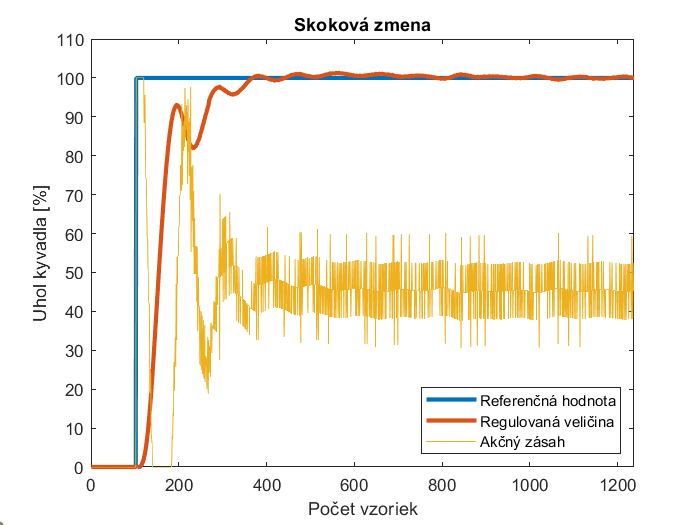
\includegraphics[width=120mm]{obr/SkokovaZmena.png}
	\caption{Reakcia systému na skokovú zmenu referenčnej hodnoty- Arduino IDE.}\label{OBRAZOK 2.5.1}
\end{figure}

Manuálna trajektória obr.\ref{OBRAZOK 2.5.3}, má oproti automatickej trajektórii obr.\ref{OBRAZOK 2.5.2}, väčšie rozdiely v hodnote akčného zásahu. Je to spôsobené kontinuálnou zmenou referenčnej hodnoty, ako aj miernym šumom signálu z potenciometra. V rámci obr.\ref{OBRAZOK 2.5.3} si ešte môžeme všimnúť časť medzi vzorkami 5000-6000. Ide o manuálne zavedenie chyby, pomocou buchnutia do kyvadla. Systém na takúto zmenu reaguje zmenou akčného zásahu a regulačnú odchýlku menšiu ako 2\%, nadobúda v priebehu jednej sekundy. 

\begin{figure}[!tbh]
	\centering
	\includegraphics[width=150mm]{obr/Auto3.png}
	\caption{Automatická trajektória.}\label{OBRAZOK 2.5.2}
\end{figure}

\begin{figure}[!tbh]
	\centering
	\includegraphics[width=150mm]{obr/potentio.png}
	\caption{Manuálna trajektória.}\label{OBRAZOK 2.5.3}
\end{figure}


\subsection{MATLAB}
\label{MATLABPID}

Príklad na ukážku fungovania PID regulátora bol taktiež vytvorený v prostredí MATLAB a simulink. V prípade MATLABU využívame, na výpočet akčného zásahu, knižnicu PID.m, ktorá bola taktiež vytvorená v rámci programu AutomationShield. Na nastavenie parametrov PID slúži príkaz \code{PID.setParameters(Kp, Ti, Td, Ts)}. 

Na vzorkovanie využívame funkcie \verb|TIC a TOC |, ktoré merajú prejdený čas. Funkcia TIC zaznamenáva aktuálny čas a funkcia TOC používa zaznamenanú hodnotu na výpočet uplynulého času. Ak je splnená podmienka \code{if (toc>=Ts*k)}, povolí sa posun na nasledujúcu vzorku, pričom premenná \verb*|k|, udáva počet vykonaných vzoriek. Dáta sú postupne zapisované do poľa \code{ PIDresponse(k,:)=[r y u]}, a toto pole je vykresľované pomocou funkcie \code{plotLive(PIDresponse(k,:))}. Na konci sú všetky dáta uložené, a teda sú prístupné aj po ukončený programu. Kompletný zdrojový kód sa nachádza v prílohe \ref{AeroShieldPID.m}.

Regulácia PID v prostredí MATLAB potrebuje pre svoje fungovanie pomerne vysoký výpočtový výkon počítača, pretože výpočty prebiehajú na zariadení, s ktorým je Arduino prepojené. Na zariadení \cite{Notebook} v ktorom boli písané všetky didaktické príklady dosahujeme rýchlosť maximálne piatich vzoriek za sekundu tj. Ts=0.2s. Pri pomalšom vzorkovaní musíme spomaliť aj rýchlosť reakcie PID regulátora (napr. znížením proporcionálnej zložky), inak regulácia prestane byť možná. Výpočtová náročnosť sa dá znížiť, zamedzením vykresľovania grafu, alebo odstránením možnosti ukladania zaznamenaných dát. 

\begin{figure}[!tbh]
	\centering
	\includegraphics[width=90mm]{obr/jednotkovyskoskMAt.png}
	\caption{Reakcia systému na skokovú zmenu referenčnej hodnoty- MATLAB.}\label{OBRAZOK 2.6.1}
\end{figure}

\subsubsection{Výstupy}

Všetky výstupy z príkladu \ref{MATLABPID}, majú priamu funkciu vykresľovania grafov spolu s legendou výstupov. Tieto grafy majú taktiež definovaný rozsah zobrazovaných hodnôt na oboch osiach, ako aj pomenovania týchto osí. Na Obr. \ref{OBRAZOK 2.6.1} vidíme reakciu systému na jednotkový skok. Obrázok \ref{OBRAZOK 2.6.2} zobrazuje automatickú trajektóriu referenčnej hodnoty a Obr. \ref{OBRAZOK 2.6.3} trajektóriu manuálnu. 

Pri manuálnej trajektórii bola trikrát vnesená veľká chyba a to pomocou úderu do kyvadla. Ako je vidieť z grafu \ref{OBRAZOK 2.6.3}, ustálenie systému prebieha oveľa pomalšie ako v príklade \ref{Arduino IDE PID}. Oscilácia je pomerne vysoká a pretrváva po dobu cca 35 vzoriek, čo predstavuje približne 7 sekúnd. Táto skutočnosť je spôsobená pomalšou reakciou PID regulátora, na veľkú regulačnú odchýlku. Dlhší čas potrebný na ustálenie kyvadla je spôsobený predovšetkým pomalším vzorkovaním. 

\begin{figure}[!tbh]
	\centering
	\includegraphics[width=125mm]{obr/PIDautomaMat.png}
	\caption{Automatická trajektória.}\label{OBRAZOK 2.6.2}
\end{figure}
\begin{figure}[!tbh]
	\centering
	\includegraphics[width=125mm]{obr/pidmanualbuchh.png}
	\caption{Manuálna trajektória.}\label{OBRAZOK 2.6.3}
\end{figure}

\newpage 
\subsection{Simulink}

Vzhľadovo pôsobí príklad PID riadenia v API Simulink jednoducho a elegantne. Predpripravené bloky z knižnice AeroLibrary stačí v príklade pospájať podľa potreby a následne zvoliť vhodné parametre v maskách blokov. Prepájanie blokov slúži na spájanie vstupov s výstupmi, alebo na matematické operácie s premennými. Regulovanú sústavu v tomto príklade predstavuje blok \verb|AeroShield|, do ktorého vstupuje z bloku \verb|Reference read| percentuálna hodnota referenčnej trajektórie. Z bloku \verb|AeroShield| získavame ako výstup uhol kyvadla, ktorý využívame na výpočet regulačnej odchýlky.  

Blok \verb|Discrete PID Controller| predstavuje riadiaci systém PID regulátora. Hodnoty jednotlivých zložiek regulátora sú: P=0.011, I=200, D=8. Matematická reprezentácia výpočtového algoritmu ideálneho PID regulátora, je v tvare Rov. \ref{PIDSimulink}:

\begin{equation}\label{PIDSimulink}
	P\left(1+I*T_s\dfrac{1}{z-1}+D*\dfrac{1}{T_s}\dfrac{z-1}{z}\right)
\end{equation}


\begin{figure}[!tbh]
	\centering
	\includegraphics[width=125mm]{obr/SimulinkPID.png}
	\caption{Ukážka riadenia systému pomocou PID regulátora v API Simulink.}\label{OBRAZOK 2.6.10}
\end{figure}

\subsubsection{Výstupy}

\begin{figure}[!tbh]
	\centering
	\includegraphics[width=100mm]{obr/SimSkok.png}
	\caption{Reakcia systému na skokovú zmenu referenčnej hodnoty- Simulink.}\label{OBRAZOK 2.6.11}
\end{figure}

\begin{figure}[!tbh]
	\centering
	\includegraphics[width=125mm]{obr/SimulinkManualBuch.png}
	\caption{Manuálna trajektória.}\label{OBRAZOK 2.6.12}
\end{figure}
\chapter{Záver}

 V rámci bakalárskej práce boli vytvorené 2 verzie AeroShieldu R2 \ref{PCBcka} a R3 \ref{tretia}, ako aj jeho spojovacie prvky a telo kyvadla \ref{telo}. Zároveň boli vytvorené a otestované 3 knižnice AeroShieldu a to pre API Arduino IDE \ref{ArduinoLib}, MATLAB \ref{matlabik} a Simulink \ref{SimulinkLib}. Na ukážku funkcií z knižníc boli vytvorené príklady v otvorenej slučke bez spätnej väzby \ref{bezspatnej}, ako aj príklady v uzatvorenej slučke so spätnou väzbou \ref{sospatnou}. Týmito príkladmi sme potvrdili funkčnosť AeroShieldu v API Arduino IDE, MATLAB a Simulink. AeroShield je teda použiteľný ako didaktická pomôcka a to aj napriek niektorým nedostatkom na softvérovom, ako aj hardvérovom rozhraní. 

Na AeroShielde je zaznamenávaný prúd, ktorý odoberá akčný člen sústavy. Toto meranie je pri malých zmenách prúdu pomerne nepresné a to z dôvodu ovládania motora PWM signálom. V budúcej verzii AeroShieldu môže byť použitý iný druh napájania motora, čo by malo za následok aj vylepšenie presnosti merania prúdu. Takto nameraný prúd by sa dal následne využívať na presnejšie riadenie výkonu motora, alebo na implementáciu PID regulácie na základe prúdu a nie uhlu kyvadla. Momentálne sa pracuje na vylepšení výstupu z merania prúdu pomocou metódy filtrácie (low pass filter).

Ďalším problémom pri PID regulácii AeroShieldu je jeho zložité a dlhotrvajúce nastavenie parametrov v API Arduino IDE a MATLABE. Problémom bolo taktiež pomalšie vzorkovanie v príklade \ref{matlabik}, ako aj nelineárne správanie sústavy.

Priame prepojenie motora so Shieldom taktiež spôsobuje isté nepríjemnosti. V prípade nechceného pretočenia ramena kyvadla sa napájacie káble zapletú na rameno a to spôsobí zamedzenie ďalšieho otáčania. Všetky didaktické príklady síce majú implementovanú softvérovú ochranu proti takémuto pretočeniu, avšak táto nie je 100\% účinná. 
Tento problém by vyriešila realizácia napájania pomocou konektora so zbernými krúžkami, avšak takýto konektor stojí v priemere 15\euro, a teda jeho aplikácia v nízko nákladovej učebnej pomôcke je otázna. Zároveň pomocou magnetu uloženého na konci kyvadla meriame jeho uhol. Použitý konektor by preto musel mať stredovú časť s možnosťou pripevnenia magnetu, alebo by sa uhol kyvadla musel merať iným spôsobom. 

Medzi vylepšenia nasledujúceho modelu AeroShieldu môžeme zaradiť úplnú zmenu podporného systému kyvadla. Uchytenie pomocou dvoch otočených \verb|V| konštrukcií prepojených priečkou by umožňovalo meranie natočenia na jednej strane priečky a druhou stranou by bolo realizované napájanie motora.   

Medzi dalšie vylepšenia pre budúcu prácu s AeroShieldom môžeme zaradiť reguláciu pomocou iného algoritmu ako bol PID. Medzi ne môžeme zaradiť modelové prediktívne riadenie (MPC), Lineárno-kvadratické riadenie (LQ), Lineárne riadenie s premenlivým parametrom (LPV), ,,fuzzy'' PID a mnoho ďalších. Pomocou týchto algoritmov by sme mohli dosiahnuť lepšie vlastnosti systému a tým pádom presnejšie riadenie. 

Všetky chyby a nedokonalosti dizajnu, ako aj neschopnosť dokonalého nastavenia uhlu kyvadla pri PID regulácii,
neznemožňujú kvalitnú výuku s použitím AeroShieldu. Jedná sa skôr o nápady a možnosti vylepšenia, ktoré môžu byť v budúcnosti na AeroShield implementované.

%%%%%%% Koniec %%%%%%%%

\bibliographystyle{unsrt}
\addcontentsline{toc}{chapter}{Literat\'{u}ra}
\bibliography{bibliog}
\backmatter
\pagenumbering{roman}\setcounter{page}{4}
\cleardoublepage
% \phantomsection
\addcontentsline{toc}{chapter}{Arduino IDE}
\addcontentsline{toc}{section}{Zdrojový kód AeroShield.h}
\LARGE\bf{Zdrojový kód súboru AeroShield.h}
\label{AeroShield.h}
\vspace{1cm}
\begin{lstlisting}[numbers=left,basicstyle=\scriptsize,caption={Zdrojový kód súboru AeroShield.h.},captionpos=b,]	
	#ifndef AEROSHIELD_H			 
	#define AEROSHIELD_H	
	
	#include "AutomationShield.h" 
	#include <Wire.h>              
	#include <Arduino.h>			 
	#define AERO_RPIN A3        
	#define VOLTAGE_SENSOR_PIN A2   
	#define AERO_UPIN 5   
	
	class AeroShield{		    	               
		public:
		AeroShield(void);
		void begin(void);                                       
		void actuatorWrite(float PotPercent);          
		float calibration(word RawAngle);          
		float convertRawAngleToDegrees(word newAngle);  
		float referenceRead(void);
		float currentMeasure(void);
		int detectMagnet();	
		int getMagnetStrength();
		word getRawAngle();
		
		private:
		int ang;                                        
		float startangle;                              
		float referenceValue;               
		float referencePercent;              
		float correction1= 4.1220;			
		float correction2= 0.33;			
		int repeatTimes= 100;				
		float voltageReference= 5.0;		
		float ShuntRes= 0.1;				
		float current;						
		float voltageValue;				
		int _ams5600_Address = 0x36;	
		int _stat = 0x0b;				
		int _raw_ang_hi = 0x0c;		
		int _raw_ang_lo = 0x0d;		
		int readOneByte(int in_adr);	
		word readTwoBytes(int in_adr_hi, int in_adr_lo); 
	};
	#endif
\end{lstlisting}
\addcontentsline{toc}{section}{Zdrojový kód AeroShield.cpp}
\LARGE\bf{Zdrojový kód súboru AeroShield.cpp}
\label{AeroShield.cpp}
\vspace{1cm}
\begin{lstlisting}[numbers=left,basicstyle=\tiny,caption={Zdrojový kód súboru AeroShield.cpp.},captionpos=b]	
	#include "AeroShield.h"     
	
	void AeroClass::begin(void){                     
		bool isDetected = AeroShield.detectMagnet();
		pinMode(AERO_UPIN,OUTPUT);  
		
		#ifdef ARDUINO_ARCH_AVR  
		Wire.begin();                                      
		#elif ARDUINO_ARCH_SAM 
		Wire1.begin();     
		#elif ARDUINO_ARCH_SAMD   
		Wire.begin();    
		#endif
		if(isDetected == 0 ){ 
			while(1){     
				if(isDetected == 1 ){  
					AutomationShield.serialPrint("Magnet detected \n");
					break;
				}
				else{      
					AutomationShield.serialPrint("Can not detect magnet \n"); 
				}
			}
		}       
	} 
	
	float AeroShield::convertRawAngleToDegrees(word newAngle) {
		float retVal = newAngle * 0.087;      
		ang = retVal;                               
		return ang;                  
	}
	
	float AeroShield::calibration(word RawAngle) {      
		AutomationShield.serialPrint("Calibration running...\n");  
		startangle=0;                                
		analogWrite(AERO_UPIN,50);              
		delay(250);                              
		analogWrite(AERO_UPIN,0);              
		delay(4000);    
		
		startangle = RawAngle;                                 
		analogWrite(AERO_UPIN,0);                     
		for(int i=0;i<3;i++){                  
			analogWrite(AERO_UPIN,1);                 
			delay(200);                           
			analogWrite(AERO_UPIN,0);                                
			delay(200);                                     
		}
		AutomationShield.serialPrint("Calibration done");
		return startangle;                                         
	}
	
	float AeroShield::referenceRead(void) {                                                
		referencePercent = AutomationShield.mapFloat(analogRead(AERO_RPIN), 0.0, 1024.0, 0.0, 100.0);   
		return referencePercent;                                     
	}
	
	void AeroShield::actuatorWrite(float PotPercent) {       
		float mappedValue = AutomationShield.mapFloat(PotPercent, 0.0, 100.0, 0.0, 255.0);  
		mappedValue = AutomationShield.constrainFloat(mappedValue, 0.0, 255.0);
		analogWrite(AERO_UPIN, (int)mappedValue);    
	}
	
	float AeroShield::currentMeasure(void){       
		for(int i=0 ; i<repeatTimes ; i++){                                            
			voltageValue= analogRead(VOLTAGE_SENSOR_PIN);                                       
			voltageValue= (voltageValue * voltageReference) / 1024;                             
			current= current + correction1-(voltageValue / (10 * ShuntRes));     
		}                                                              
		float currentMean= current/repeatTimes;             
		currentMean= currentMean-correction2;              
		if(currentMean < 0.000){                           
			currentMean= 0.000;                             
		}
		current= 0;               
		voltageValue= 0;         
		return currentMean;  
	}
	
	word AeroShield::getRawAngle()                                                           
	{
		return readTwoBytes(_raw_ang_hi, _raw_ang_lo);                                         
	}
	
	int AeroShield::detectMagnet()                                                         
	{
		int magStatus;                                                                   
		int retVal = 0;                                                                      
		magStatus = readOneByte(_stat);                                                                  
		if (magStatus & 0x20)
		retVal = 1;
		return retVal;                                                               
	}
	
	int AeroShield::getMagnetStrength()           
	{
		int magStatus;                                 
		int retVal = 0;                             
		magStatus = readOneByte(_stat);               
		if (detectMagnet() == 1)                         
		{	retVal = 2;                               
			if (magStatus & 0x10)
			retVal = 1;                               
			else if (magStatus & 0x08)
			retVal = 3;                            
		} return retVal;                          
	}
	
	int AeroShield::readOneByte(int in_adr)       
	{
		int retVal = -1;
		Wire.beginTransmission(_ams5600_Address);     
		Wire.write(in_adr);                            
		Wire.endTransmission();                         
		Wire.requestFrom(_ams5600_Address, 1);          
		while (Wire.available() == 0);                   
		retVal = Wire.read();                         
		return retVal;                                   
	}
	
	word AeroShield::readTwoBytes(int in_adr_hi, int in_adr_lo)     
	{
		word retVal = -1;
		/* Read Low Byte */
		Wire.beginTransmission(_ams5600_Address);     
		Wire.write(in_adr_lo);                        
		Wire.endTransmission();                        
		Wire.requestFrom(_ams5600_Address, 1);          
		while (Wire.available() == 0);                  
		int low = Wire.read();                    
		
		/* Read High Byte */
		Wire.beginTransmission(_ams5600_Address);       
		Wire.write(in_adr_hi);                    
		Wire.endTransmission();                       
		Wire.requestFrom(_ams5600_Address, 1);        
		while (Wire.available() == 0);               
		word high = Wire.read();                    
		high = high << 8;                             
		retVal = high | low;
		return retVal;                                
	}	
\end{lstlisting}
\addcontentsline{toc}{section}{Zdrojový kód AeroShieldOpenLoop.ino}
\LARGE\bf{Zdrojový kód súboru AeroShieldOpenLoop.ino}
\label{AeroShieldOpenLoop.ino}
\vspace{1cm}
\begin{lstlisting}[numbers=left,basicstyle=\scriptsize,caption={Zdrojový kód súboru AeroShieldOpenLoop.ino.},captionpos=b]	
	#include "AeroShield.h" 
	
	float startAngle=0; 
	float lastAngle=0; 
	float pendulumAngle;  
	float referencePercent;  
	float CurrentMean; 
	
	void setup() {
		
		Serial.begin(115200);   
		AeroShield.begin(AeroShield.detectMagnet());
		startAngle = AeroShield.calibration(AeroShield.getRawAngle());
		lastAngle=startAngle+1024;  
	}
	
	void loop() {
		if(pendulumAngle>120){
			AeroShield.actuatorWrite(0);
			while(1);
		}
		
	pendulumAngle= AutomationShield.mapFloat(AeroShield.getRawAngle(),startAngle,lastAngle,0.00,90.00);  
	referencePercent= AeroShield.referenceRead(); 
	AeroShield.actuatorWrite(referencePercent);    
	CurrentMean= AeroShield.currentMeasure();

	Serial.print(pendulumAngle);  
	Serial.print(" ");
	Serial.print(referencePercent); 
	Serial.print(" ");
	Serial.println(CurrentMean);
	}
\end{lstlisting}
\addcontentsline{toc}{section}{Zdrojový kód AeroShieldPID.ino}
\LARGE\bf{Zdrojový kód súboru AeroShieldPID.ino}
\label{AeroShieldPID.ino}
\vspace{1cm}
\begin{lstlisting}[numbers=left,basicstyle=\scriptsize,caption={Zdrojový kód súboru AeroShieldPID.ino.},captionpos=b]	
	#include "AeroShield.h"              
	#include <Sampling.h>   
	
	#define MANUAL 0    
	#define KP 1.7  
	#define TI 3.8  
	#define TD 0.25   
	
	float startangle=0; 
	float lastangle=0; 
	float pendulumAngle;
	
	unsigned long Ts = 3; 
	unsigned long k = 0; 
	bool nextStep = false;  
	bool realTimeViolation = false;
	
	int i=i;          
	int T=1000;           
	float R[]={45.0,23.0,75.0,32.0,58.0,10.0,35.0,19.0,9.0,43.0,23.0,65.0,15.0,80.0}; 
	float r=0.0;          
	float y = 0.0;        
	float u = 0.0;         
	
	void setup() {           
		Serial.begin(250000);                         
		AeroShield.begin(AeroShield.detectMagnet());
		startangle = AeroShield.calibration(AeroShield.getRawAngle()); 
		lastangle=startangle+1024;                                  
		Sampling.period(Ts*1000);      
		PIDAbs.setKp(KP);       
		PIDAbs.setTi(TI);    
		PIDAbs.setTd(TD);     
		PIDAbs.setTs(Sampling.samplingPeriod); 
		Sampling.interrupt(stepEnable); 
	}
	
	void loop() {
		if(pendulumAngle>120){
			AeroShield.actuatorWrite(0);
			while(1);
		} 
		if (nextStep) {    
			step();          
			nextStep = false;  
		}
	}
	
	void stepEnable() {             
		if(nextStep == true) {         
			realTimeViolation = true;   
			Serial.println("Real-time samples violated."); 
			analogWrite(5,0);  
			while(1);    
		}
		nextStep = true; 
	}
	
	void step() {  
		#if MANUAL                       
		r = AeroShield.referenceRead(); 
		#else        
		if(i>(sizeof(R)/sizeof(R[0]))) {  
			analogWrite(5,0); 
			while(1); 
		} else if (k % (T*i) == 0) {
			r = R[i];
			i++; 
		}
		#endif
		y= AutomationShield.mapFloat(AeroShield.getRawAngle(),startangle,lastangle,0.00,100.00);
		u = PIDAbs.compute(r-y,0,100,0,100);
		AeroShield.actuatorWrite(u);
		
		Serial.print(r);
		Serial.print(", ");
		Serial.print(y); 
		Serial.print(", ");
		Serial.println(u); 
		k++; 
	}
\end{lstlisting}
\addcontentsline{toc}{chapter}{MATLAB}
\addcontentsline{toc}{section}{Zdrojový kód AeroShield.m}
\LARGE\bf{Zdrojový kód súboru AeroShield.m}
\label{AeroShield.m}
\vspace{1cm}
\begin{lstlisting}[numbers=left,basicstyle=\scriptsize,caption={Zdrojový kód súboru AeroShield.m.},captionpos=b]	
	classdef AeroShield < handle
	
	properties
	arduino;
	as5600;
	end
	properties(Constant)
	AERO_UPIN = 'D5'; 
	AERO_RPIN = 'A3';
	VOLTAGE_SENSOR_PIN = 'A2';
	voltageReference = 5.0;
	ShuntRes = 0.1;
	correction1 = 4.1220;
	correction2 = 0.33;
	repeatTimes = 50;
	end
	
	methods
	function begin(AeroShieldObject) 
	AeroShieldObject.arduino = arduino();
	AeroShieldObject.as5600 = device(AeroShieldObject.arduino,'I2CAddress',0x36); 
	configurePin(AeroShieldObject.arduino,AeroShieldObject.AERO_UPIN, 'DigitalOutput') 
	disp('AeroShield initialized.') 
	end
	function startangle = calibration(AeroShieldObject)
	write(AeroShieldObject.as5600, 0x0c, 'uint8');
	write(AeroShieldObject.as5600, 0x0d, 'uint8');
	startangle = read(AeroShieldObject.as5600, 1, 'uint16');
	end
	function PWM = referenceRead(AeroShieldObject)
	PWM= readVoltage(AeroShieldObject.arduino, AeroShieldObject.AERO_RPIN);
	end
	function actuatorWrite(AeroShieldObject, PWM) 
	writePWMVoltage(AeroShieldObject.arduino, AeroShieldObject.AERO_UPIN, PWM);
	end
	function RAW = getRawAngle(AeroShieldObject)
	write(AeroShieldObject.as5600, 0x0c, 'uint8');
	write(AeroShieldObject.as5600, 0x0d, 'uint8');
	RAW = read(AeroShieldObject.as5600, 1, 'uint16');
	end
	function currentMean = getCurrent()
	for r = 1:repeatTimes
	voltageValue = readVoltage(AeroShieldObject.arduino, AeroShieldObject.VOLTAGE_SENSOR_PIN);
	voltageValue= (voltageValue * voltageReference) / 1024;
	Current= Current + correction1-(voltageValue / (10 * ShuntRes)); 
	end
	currentMean= Current/repeatTimes;
	currentMean= currentMean-correction2;
	if currentMean < 0.000 
	currentMean= 0.000; 
	end
	current= 0;  
	voltageValue=0;   
	end 
	end
	end
\end{lstlisting}
\addcontentsline{toc}{section}{Zdrojový kód AeroShieldOpenLoop.m}
\LARGE\bf{Zdrojový kód súboru AeroShieldOpenLoop.m}
\label{AeroShieldOpenLoop.m}
\vspace{1cm}
\begin{lstlisting}[numbers=left,basicstyle=\scriptsize,caption={Zdrojový kód súboru AeroShieldOpenLoop.m.},captionpos=b]	
	clear all;
	clear a;
	clc 
	
	AeroShield=AeroShield;
	AeroShield.begin();
	startangle= AeroShield.calibration(); 
	lastangle=startangle+2048;
	
	time = 0;
	count = 0;
	angle = 0;
	potentiometer = 0;
	
	yyaxis right  
	plotGraph = plot(time,angle,'-r' )
	ylabel('Angle (degree)','FontSize',15);
	xlabel('Time (s)','FontSize',15); 
	hold on  
	
	yyaxis left 
	plotGraph1 = plot(time,potentiometer,'-b')
	title('Pendulum plot','FontSize',15);
	ylabel('Percent','FontSize',15)  
	legend('Potentiometer value','Pendulum angle')
	grid('on');
	
	tic    
	
	while ishandle(plotGraph)  
	pwm = AeroShield.referenceRead();
	AeroShield.actuatorWrite(pwm);
	
	RAW= AeroShield.getRawAngle();  
	angle_ = mapped(RAW, startangle, lastangle, 0, 180);
	count = count + 1;  
	time(count) = toc;      
	angle(count) = angle_(1);   
	percenta= mapped(pwm, 0.0, 5.0, 0.0, 100.0); 
	potentiometer(count) = percenta(1);          
	set(plotGraph,'XData',time,'YData',angle);   
	set(plotGraph1,'XData',time,'YData',potentiometer);
	axis([time(count)-5 time(count) 0 100]);  
	
	if (angle_ > 110)                         
	AeroShield.actuatorWrite(0.0);    
	disp('Angle of pendulum too high. AeroShield is turned off')
	break                              
	end
	end             
	
	clear AeroShield.arduino;
\end{lstlisting}
\addcontentsline{toc}{section}{Zdrojový kód AeroShielPID.m}
\LARGE\bf{Zdrojový kód súboru AeroShieldPID.m}
\label{AeroShieldPID.m}
\vspace{1cm}
\begin{lstlisting}[numbers=left,basicstyle=\scriptsize,caption={Zdrojový kód súboru AeroShieldPID.m.},captionpos=b]	
	clear all
	clc 
	AeroShield=AeroShield; 
	PID = PID;
	AeroShield.begin();
	startangle= AeroShield.calibration(); 
	lastangle=startangle+1024; 
	Ts = 0.0017;   
	Kp=0.015 ;
	Ti=0.00020 ;
	Td=0.0003 ;  
	PID.setParameters(Kp, Ti, Td, Ts);
	MANUAL= 0;
	R=[23 48 69 45 19 37 78];
	secLength=30; 
	stepEnable = 0;  
	k=1; 
	j=1;
	r=R(1);
	y=0;      
	
	tic 
	while(1) 
	if (stepEnable) 
	RAW = AeroShield.getRawAngle();
	y = map(RAW, startangle, lastangle, 0.0, 100.0);
	if MANUAL  
	PWMvalue = AeroShield.referenceRead(); 
	r=map(PWMvalue, 0, 5, 0, 100);
	else 
	if (mod(k,secLength*j)==0); 
	j=j+1; 
	if (j > length(R)) 
	AeroShield.actuatorWrite(0.0); 
	break  
	end
	r=R(j); 
	end
	end
	u = PID.compute(r-y, 0, 90, 0, 90); 
	coercedInput = constrain(u, 0, 100); 
	PWM=map(coercedInput, 0, 100, 0, 5); 
	AeroShield.actuatorWrite(PWM); 
	PIDresponse(k,:)=[r y u];
	plotLive(PIDresponse(k,:)); 
	k=k+1;  
	stepEnable = 0; 
	end      
	if (toc>=Ts*k)      
	stepEnable = 1;            
	end
	if (y > 110)        
	AeroShield.actuatorWrite(0.0); 
	disp('Angle of pendulum too high. AeroShield is turned off')
	break                     
	end
	end   
	
	disp('Example finished. Captured data saved to "PIDresponse.mat" file.')
	save PIDresponse PIDresponse     
\end{lstlisting}
\addcontentsline{toc}{chapter}{Simulink}
\end{document}
